\section{SiO2}
\subsection*{Material ID: mp-bamv}
\textbf{Constante Dieléctrica ($\epsilon_{total}$):} 2.89 \\[0.5em]
\begin{table}[h!]
\centering
\begin{tabular}{lcc}
\toprule
\textbf{Métrica} & \textbf{Lámina (Plate)} & \textbf{Cilindros (Rod)} \\
\midrule
Bandgaps ($k_x$) & Ninguno & Ninguno \\
Resonancias ($k_x$) & 36 & 36 \\
\midrule
Bandgaps (Rotación) & Ninguno & Ninguno \\
Resonancias (Rotación) & 33 & 33 \\
\bottomrule
\end{tabular}
\end{table}
\begin{figure}[H]
\centering
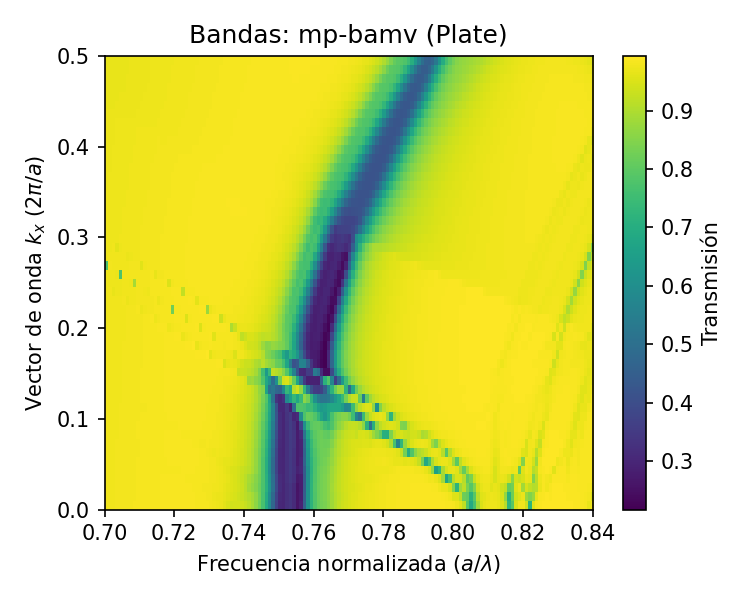
\includegraphics[width=0.48\textwidth]{figures/mp-bamv_plate.png}
\hfill
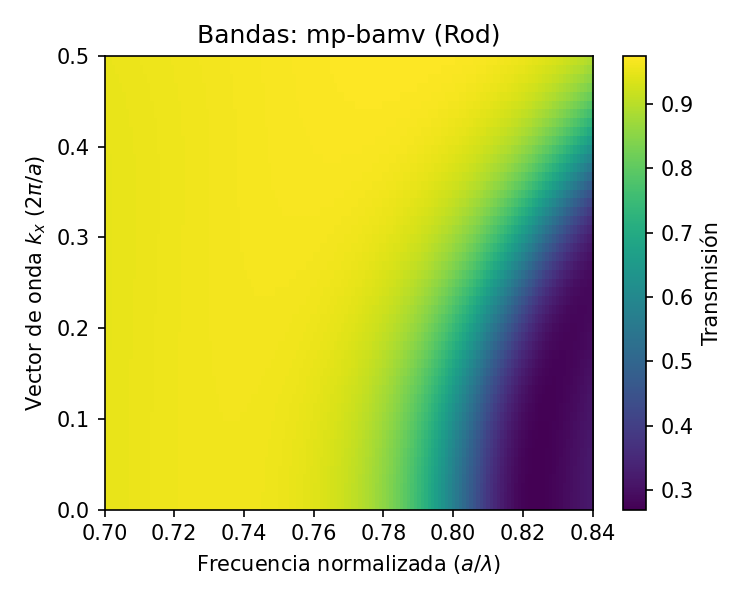
\includegraphics[width=0.48\textwidth]{figures/mp-bamv_rod.png}
\caption{Estructuras de bandas fotónicas ($k_x$) para mp-bamv. Izquierda: Lámina. Derecha: Cilindros.}
\end{figure}
\vspace{1em}
\begin{figure}[H]
\centering
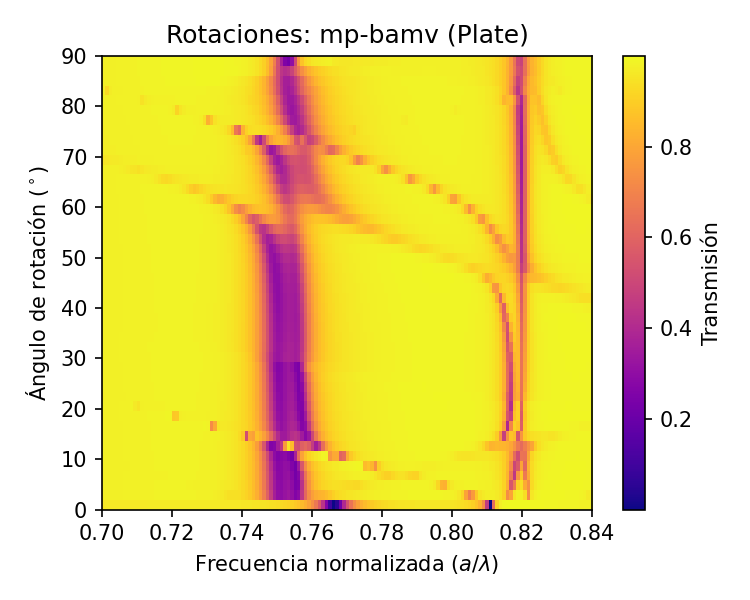
\includegraphics[width=0.48\textwidth]{figures/mp-bamv_plate_rangle.png}
\hfill
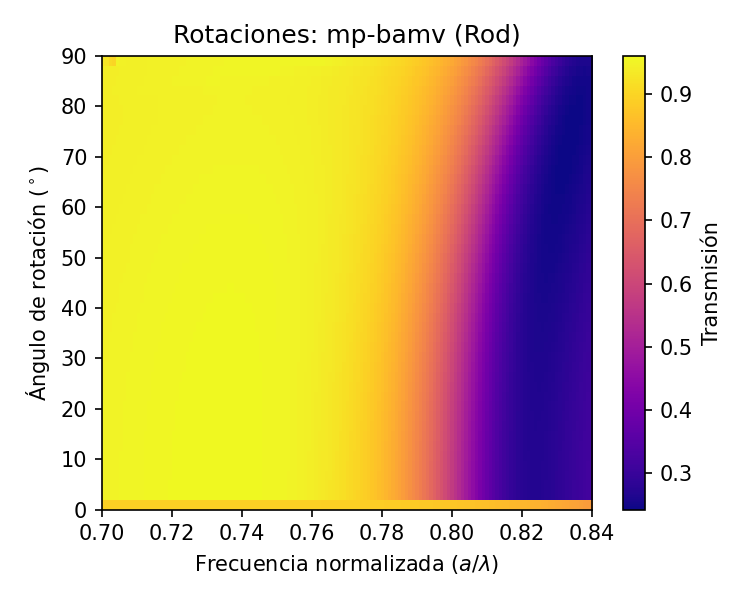
\includegraphics[width=0.48\textwidth]{figures/mp-bamv_rod_rangle.png}
\caption{Mapas de transmisión por rotación (twist) para mp-bamv. Izquierda: Lámina. Derecha: Cilindros.}
\end{figure}
\vspace{1em}
\hrule
\vspace{1em}
\subsection*{Material ID: mp-bfcna}
\textbf{Constante Dieléctrica ($\epsilon_{total}$):} 3.59 \\[0.5em]
\begin{table}[h!]
\centering
\begin{tabular}{lcc}
\toprule
\textbf{Métrica} & \textbf{Lámina (Plate)} & \textbf{Cilindros (Rod)} \\
\midrule
Bandgaps ($k_x$) & Ninguno & Ninguno \\
Resonancias ($k_x$) & 36 & 36 \\
\midrule
Bandgaps (Rotación) & Ninguno & Ninguno \\
Resonancias (Rotación) & 33 & 33 \\
\bottomrule
\end{tabular}
\end{table}
\begin{figure}[H]
\centering
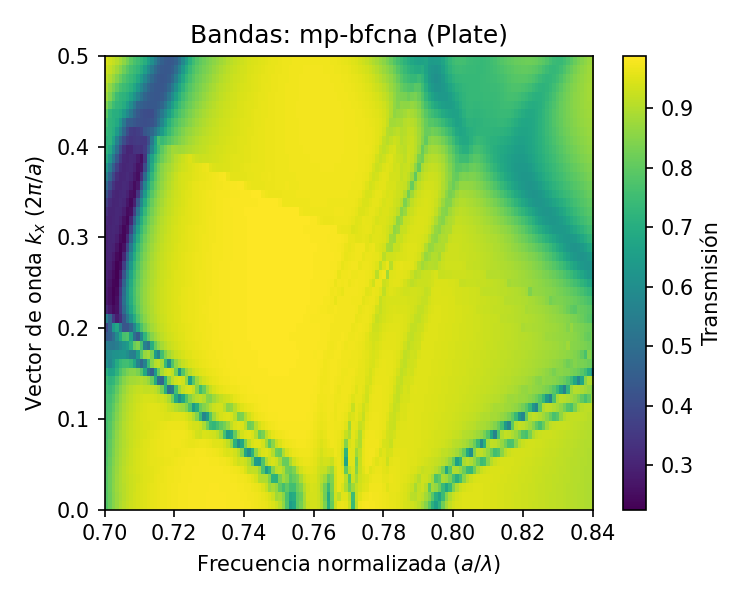
\includegraphics[width=0.48\textwidth]{figures/mp-bfcna_plate.png}
\hfill
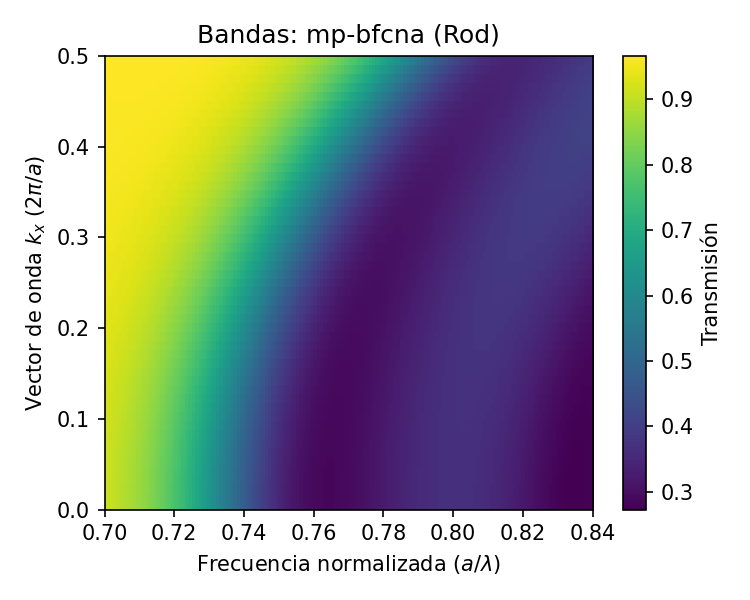
\includegraphics[width=0.48\textwidth]{figures/mp-bfcna_rod.png}
\caption{Estructuras de bandas fotónicas ($k_x$) para mp-bfcna. Izquierda: Lámina. Derecha: Cilindros.}
\end{figure}
\vspace{1em}
\begin{figure}[H]
\centering
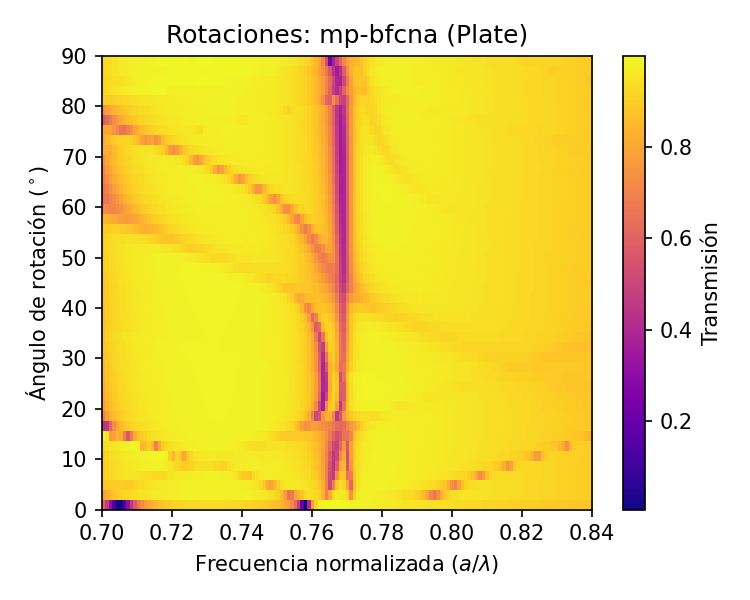
\includegraphics[width=0.48\textwidth]{figures/mp-bfcna_plate_rangle.png}
\hfill
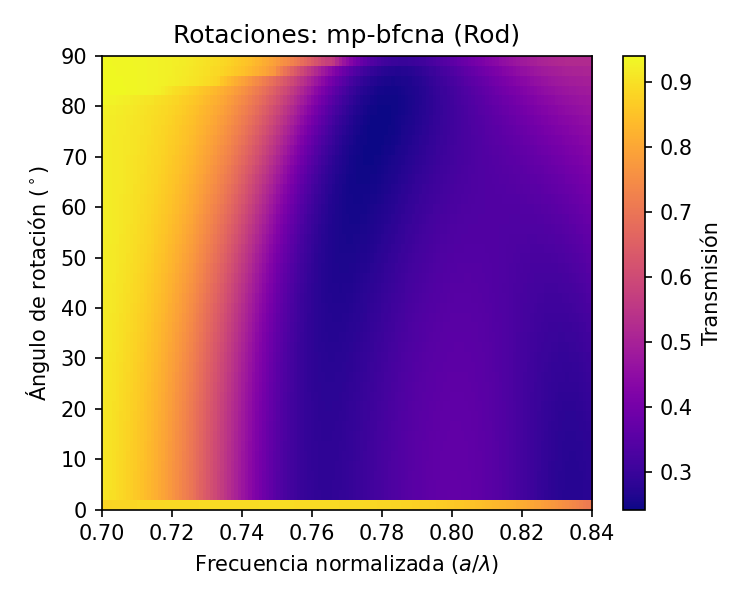
\includegraphics[width=0.48\textwidth]{figures/mp-bfcna_rod_rangle.png}
\caption{Mapas de transmisión por rotación (twist) para mp-bfcna. Izquierda: Lámina. Derecha: Cilindros.}
\end{figure}
\vspace{1em}
\hrule
\vspace{1em}
\subsection*{Material ID: mp-bfcwo}
\textbf{Constante Dieléctrica ($\epsilon_{total}$):} 3.88 \\[0.5em]
\begin{table}[h!]
\centering
\begin{tabular}{lcc}
\toprule
\textbf{Métrica} & \textbf{Lámina (Plate)} & \textbf{Cilindros (Rod)} \\
\midrule
Bandgaps ($k_x$) & Ninguno & Ninguno \\
Resonancias ($k_x$) & 36 & 36 \\
\midrule
Bandgaps (Rotación) & Ninguno & Ninguno \\
Resonancias (Rotación) & 33 & 33 \\
\bottomrule
\end{tabular}
\end{table}
\begin{figure}[H]
\centering
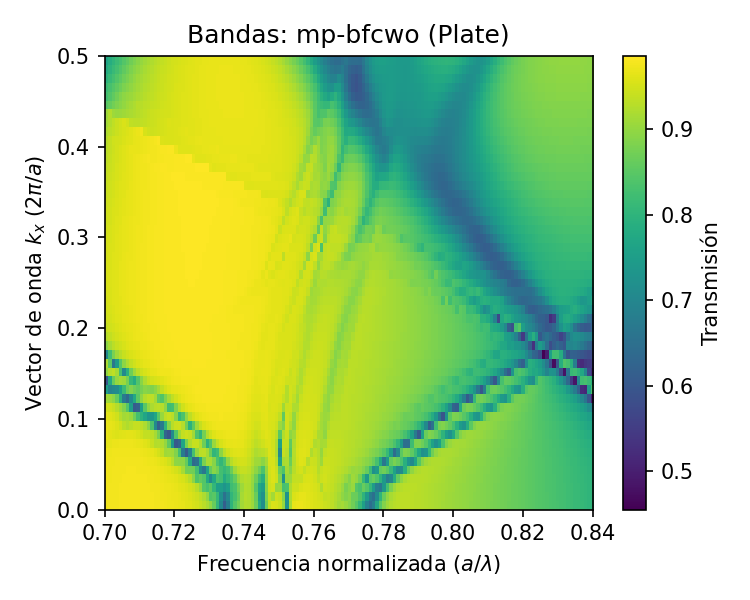
\includegraphics[width=0.48\textwidth]{figures/mp-bfcwo_plate.png}
\hfill
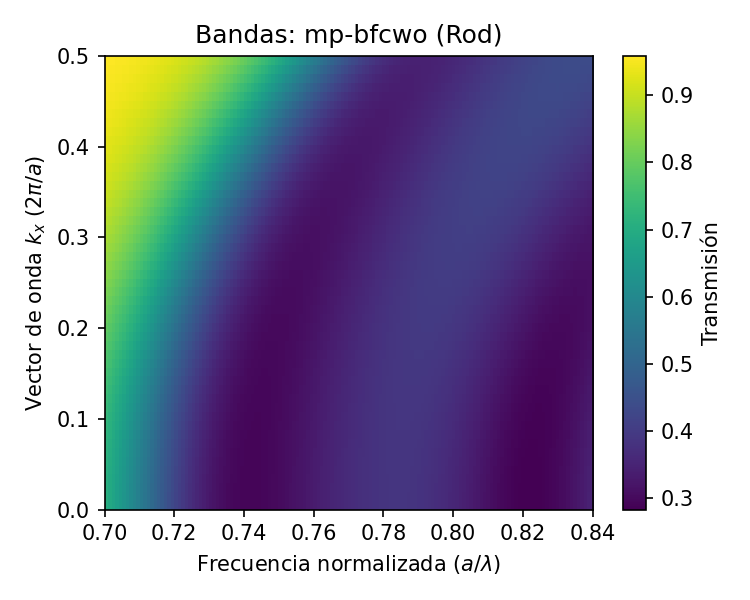
\includegraphics[width=0.48\textwidth]{figures/mp-bfcwo_rod.png}
\caption{Estructuras de bandas fotónicas ($k_x$) para mp-bfcwo. Izquierda: Lámina. Derecha: Cilindros.}
\end{figure}
\vspace{1em}
\begin{figure}[H]
\centering
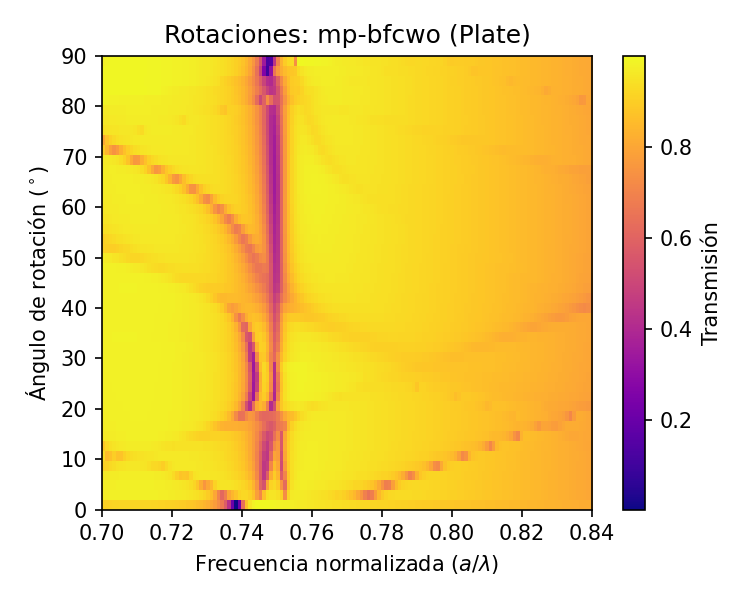
\includegraphics[width=0.48\textwidth]{figures/mp-bfcwo_plate_rangle.png}
\hfill
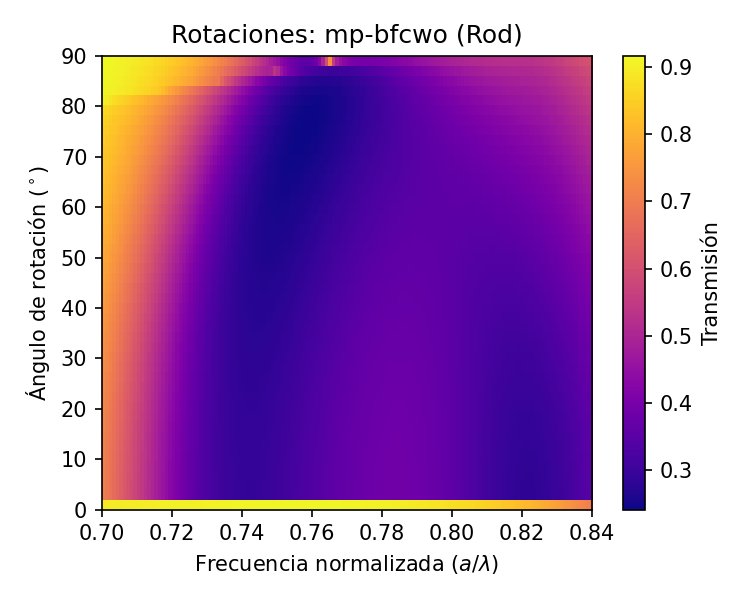
\includegraphics[width=0.48\textwidth]{figures/mp-bfcwo_rod_rangle.png}
\caption{Mapas de transmisión por rotación (twist) para mp-bfcwo. Izquierda: Lámina. Derecha: Cilindros.}
\end{figure}
\vspace{1em}
\hrule
\vspace{1em}
\subsection*{Material ID: mp-bfnrd}
\textbf{Constante Dieléctrica ($\epsilon_{total}$):} 3.99 \\[0.5em]
\begin{table}[h!]
\centering
\begin{tabular}{lcc}
\toprule
\textbf{Métrica} & \textbf{Lámina (Plate)} & \textbf{Cilindros (Rod)} \\
\midrule
Bandgaps ($k_x$) & Ninguno & Ninguno \\
Resonancias ($k_x$) & 36 & 36 \\
\midrule
Bandgaps (Rotación) & Ninguno & Ninguno \\
Resonancias (Rotación) & 33 & 33 \\
\bottomrule
\end{tabular}
\end{table}
\begin{figure}[H]
\centering
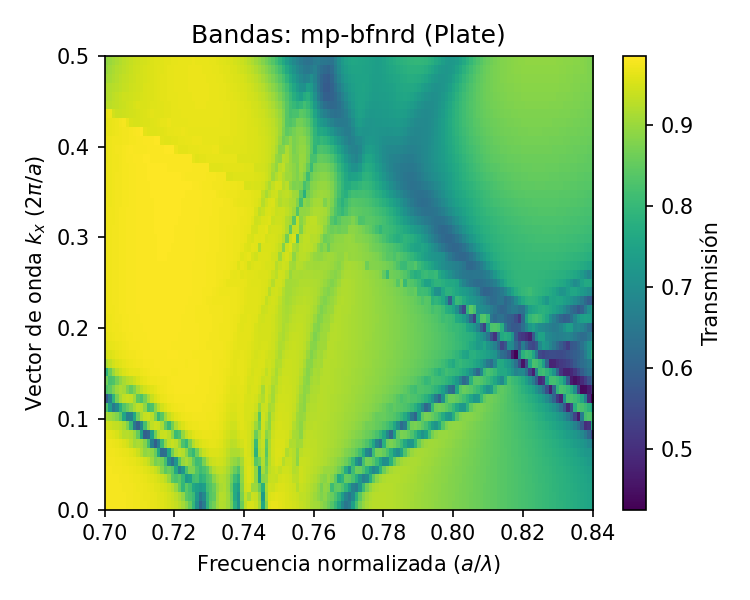
\includegraphics[width=0.48\textwidth]{figures/mp-bfnrd_plate.png}
\hfill
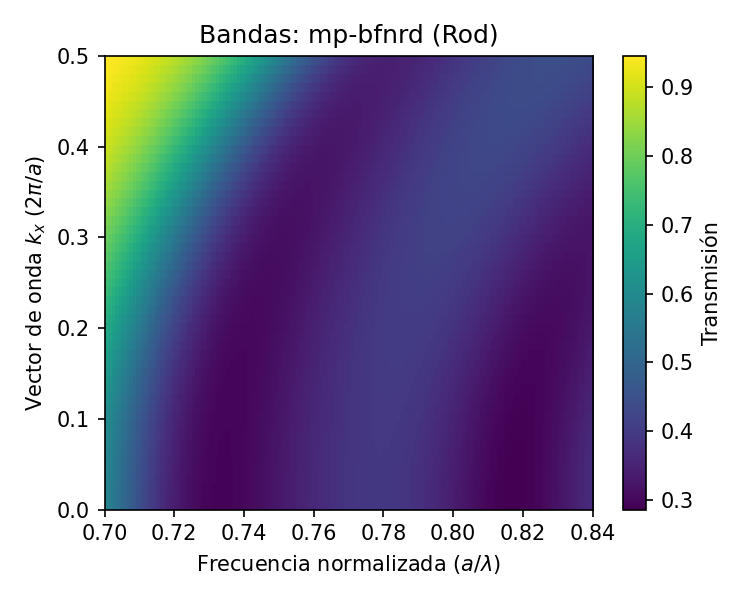
\includegraphics[width=0.48\textwidth]{figures/mp-bfnrd_rod.png}
\caption{Estructuras de bandas fotónicas ($k_x$) para mp-bfnrd. Izquierda: Lámina. Derecha: Cilindros.}
\end{figure}
\vspace{1em}
\begin{figure}[H]
\centering
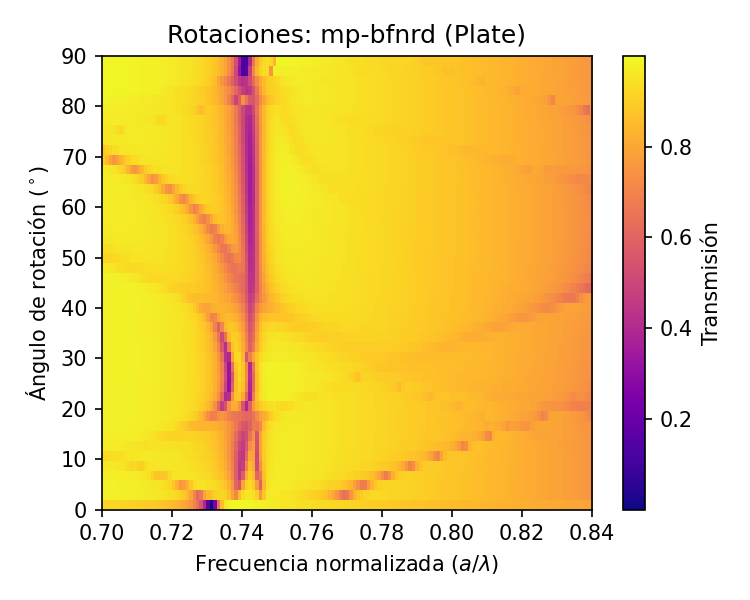
\includegraphics[width=0.48\textwidth]{figures/mp-bfnrd_plate_rangle.png}
\hfill
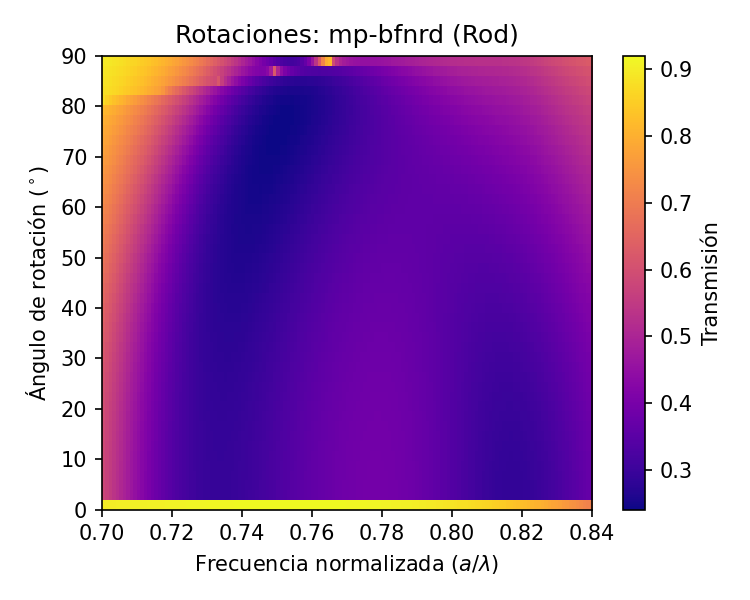
\includegraphics[width=0.48\textwidth]{figures/mp-bfnrd_rod_rangle.png}
\caption{Mapas de transmisión por rotación (twist) para mp-bfnrd. Izquierda: Lámina. Derecha: Cilindros.}
\end{figure}
\vspace{1em}
\hrule
\vspace{1em}
\subsection*{Material ID: mp-bfntn}
\textbf{Constante Dieléctrica ($\epsilon_{total}$):} 3.74 \\[0.5em]
\begin{table}[h!]
\centering
\begin{tabular}{lcc}
\toprule
\textbf{Métrica} & \textbf{Lámina (Plate)} & \textbf{Cilindros (Rod)} \\
\midrule
Bandgaps ($k_x$) & Ninguno & Ninguno \\
Resonancias ($k_x$) & 36 & 36 \\
\midrule
Bandgaps (Rotación) & Ninguno & Ninguno \\
Resonancias (Rotación) & 33 & 33 \\
\bottomrule
\end{tabular}
\end{table}
\begin{figure}[H]
\centering
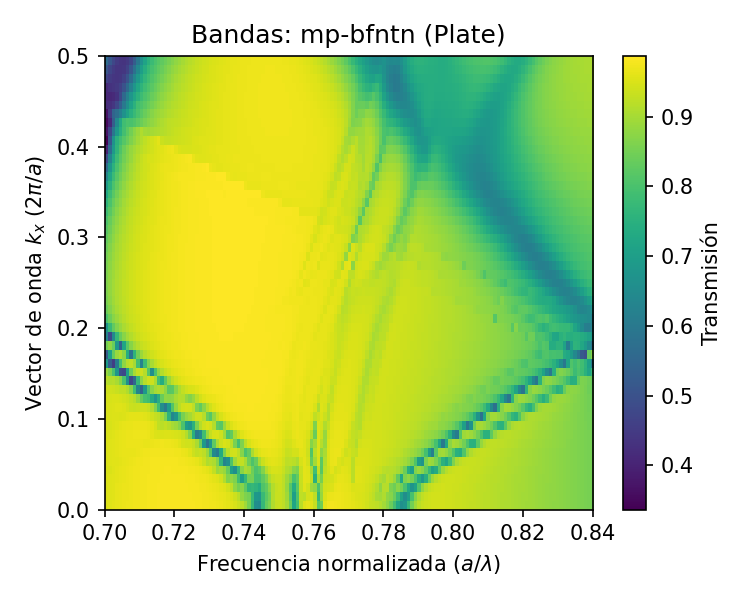
\includegraphics[width=0.48\textwidth]{figures/mp-bfntn_plate.png}
\hfill
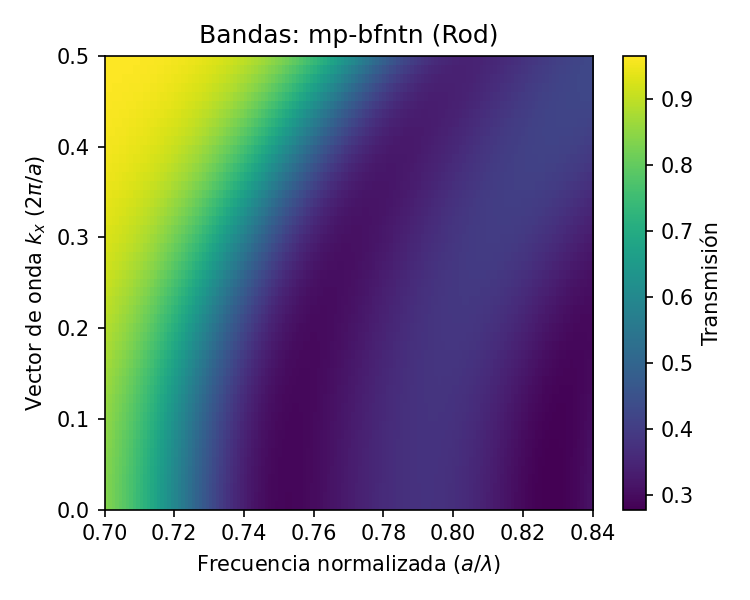
\includegraphics[width=0.48\textwidth]{figures/mp-bfntn_rod.png}
\caption{Estructuras de bandas fotónicas ($k_x$) para mp-bfntn. Izquierda: Lámina. Derecha: Cilindros.}
\end{figure}
\vspace{1em}
\begin{figure}[H]
\centering
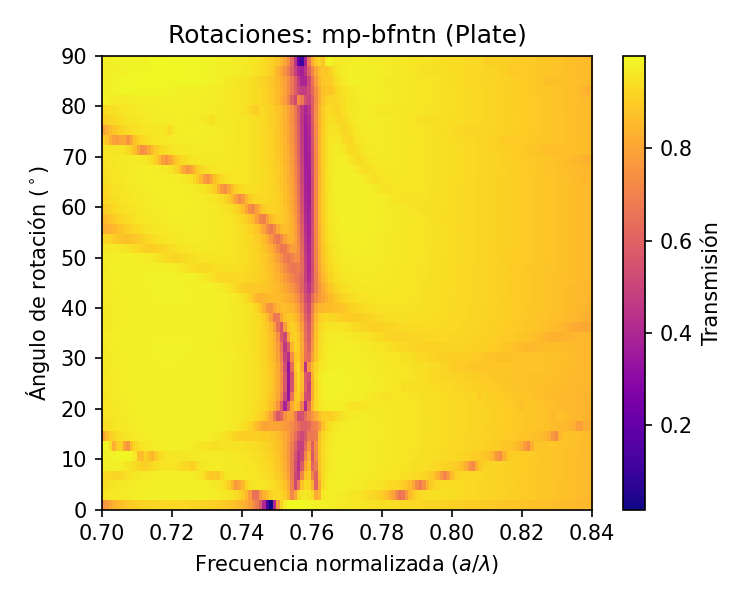
\includegraphics[width=0.48\textwidth]{figures/mp-bfntn_plate_rangle.png}
\hfill
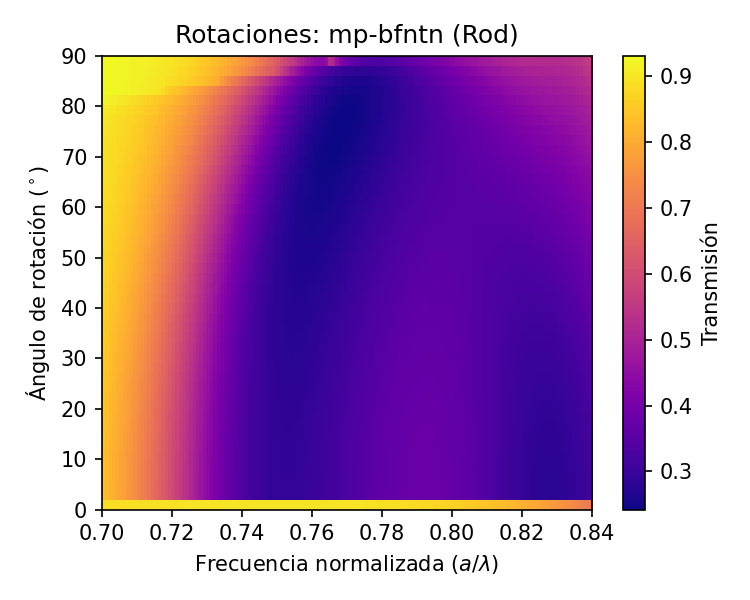
\includegraphics[width=0.48\textwidth]{figures/mp-bfntn_rod_rangle.png}
\caption{Mapas de transmisión por rotación (twist) para mp-bfntn. Izquierda: Lámina. Derecha: Cilindros.}
\end{figure}
\vspace{1em}
\hrule
\vspace{1em}
\subsection*{Material ID: mp-bfnxb}
\textbf{Constante Dieléctrica ($\epsilon_{total}$):} 3.57 \\[0.5em]
\begin{table}[h!]
\centering
\begin{tabular}{lcc}
\toprule
\textbf{Métrica} & \textbf{Lámina (Plate)} & \textbf{Cilindros (Rod)} \\
\midrule
Bandgaps ($k_x$) & Ninguno & Ninguno \\
Resonancias ($k_x$) & 36 & 36 \\
\midrule
Bandgaps (Rotación) & Ninguno & Ninguno \\
Resonancias (Rotación) & 33 & 33 \\
\bottomrule
\end{tabular}
\end{table}
\begin{figure}[H]
\centering
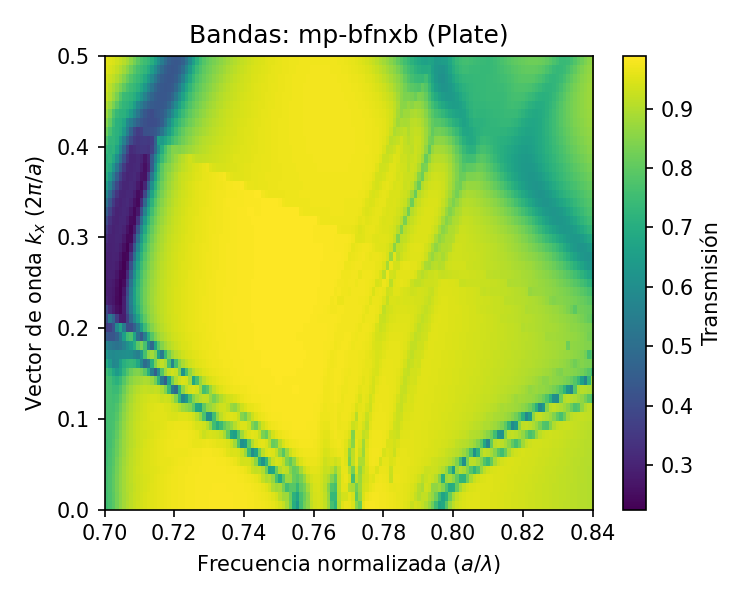
\includegraphics[width=0.48\textwidth]{figures/mp-bfnxb_plate.png}
\hfill
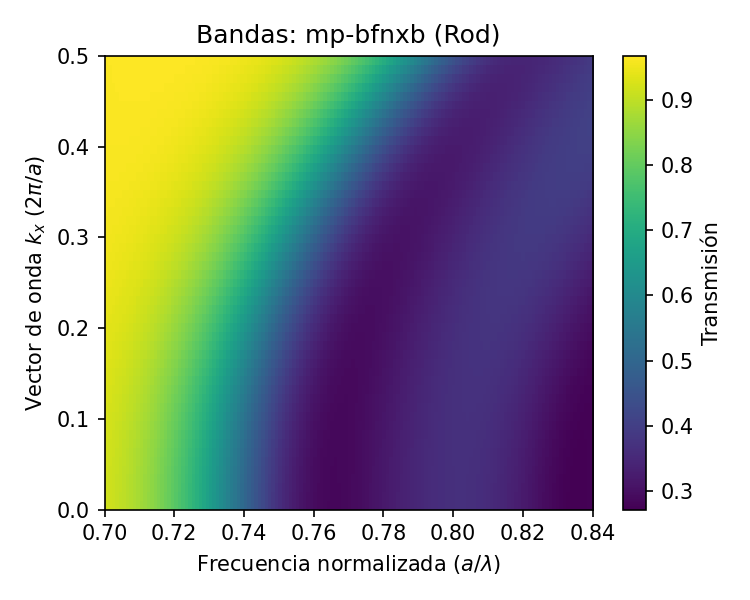
\includegraphics[width=0.48\textwidth]{figures/mp-bfnxb_rod.png}
\caption{Estructuras de bandas fotónicas ($k_x$) para mp-bfnxb. Izquierda: Lámina. Derecha: Cilindros.}
\end{figure}
\vspace{1em}
\begin{figure}[H]
\centering
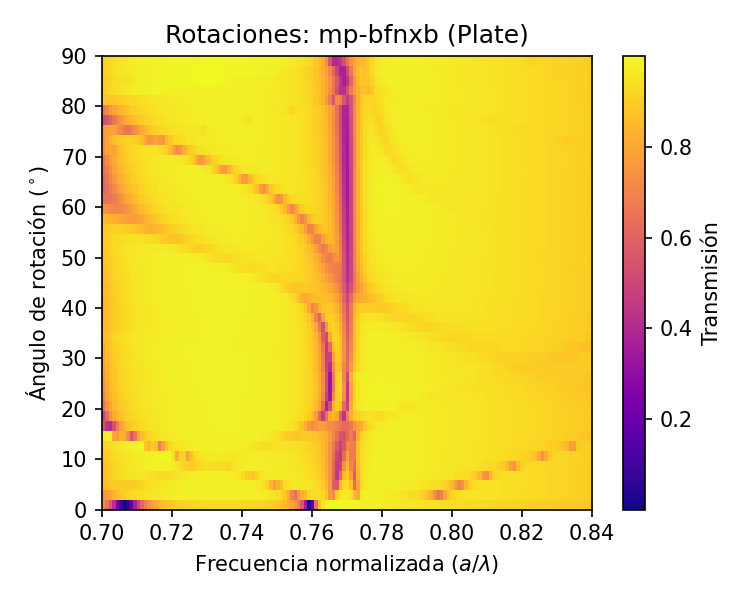
\includegraphics[width=0.48\textwidth]{figures/mp-bfnxb_plate_rangle.png}
\hfill
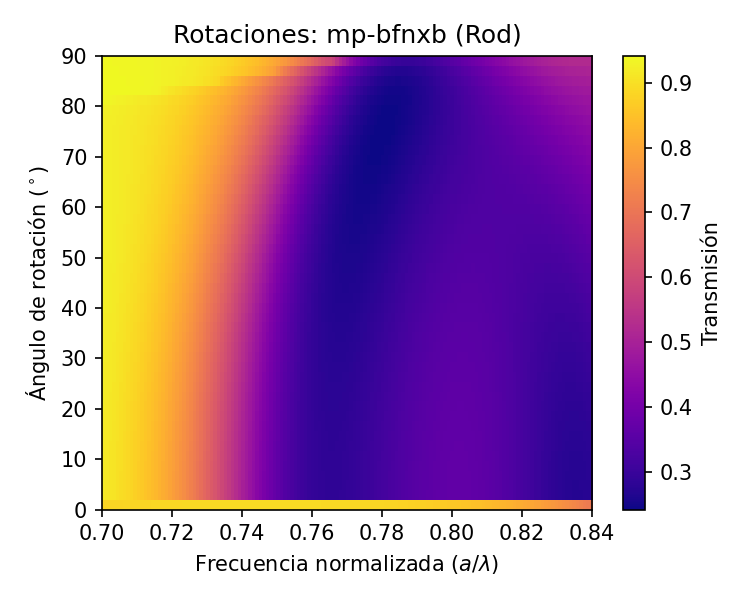
\includegraphics[width=0.48\textwidth]{figures/mp-bfnxb_rod_rangle.png}
\caption{Mapas de transmisión por rotación (twist) para mp-bfnxb. Izquierda: Lámina. Derecha: Cilindros.}
\end{figure}
\vspace{1em}
\hrule
\vspace{1em}
\subsection*{Material ID: mp-bfoip}
\textbf{Constante Dieléctrica ($\epsilon_{total}$):} 3.47 \\[0.5em]
\begin{table}[h!]
\centering
\begin{tabular}{lcc}
\toprule
\textbf{Métrica} & \textbf{Lámina (Plate)} & \textbf{Cilindros (Rod)} \\
\midrule
Bandgaps ($k_x$) & Ninguno & Ninguno \\
Resonancias ($k_x$) & 36 & 36 \\
\midrule
Bandgaps (Rotación) & Ninguno & Ninguno \\
Resonancias (Rotación) & 33 & 33 \\
\bottomrule
\end{tabular}
\end{table}
\begin{figure}[H]
\centering
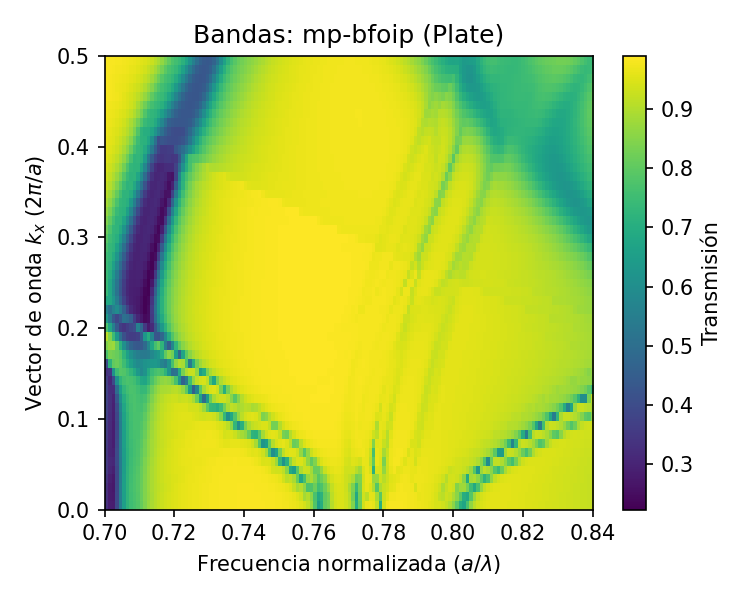
\includegraphics[width=0.48\textwidth]{figures/mp-bfoip_plate.png}
\hfill
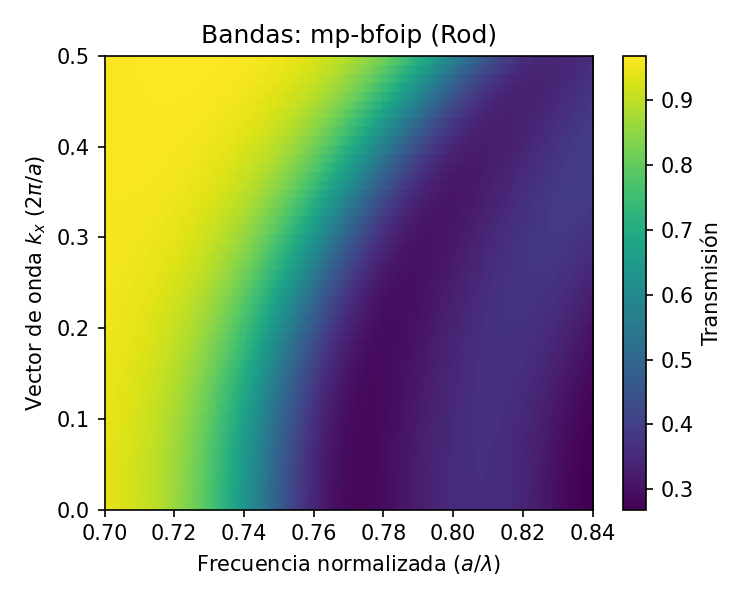
\includegraphics[width=0.48\textwidth]{figures/mp-bfoip_rod.png}
\caption{Estructuras de bandas fotónicas ($k_x$) para mp-bfoip. Izquierda: Lámina. Derecha: Cilindros.}
\end{figure}
\vspace{1em}
\begin{figure}[H]
\centering
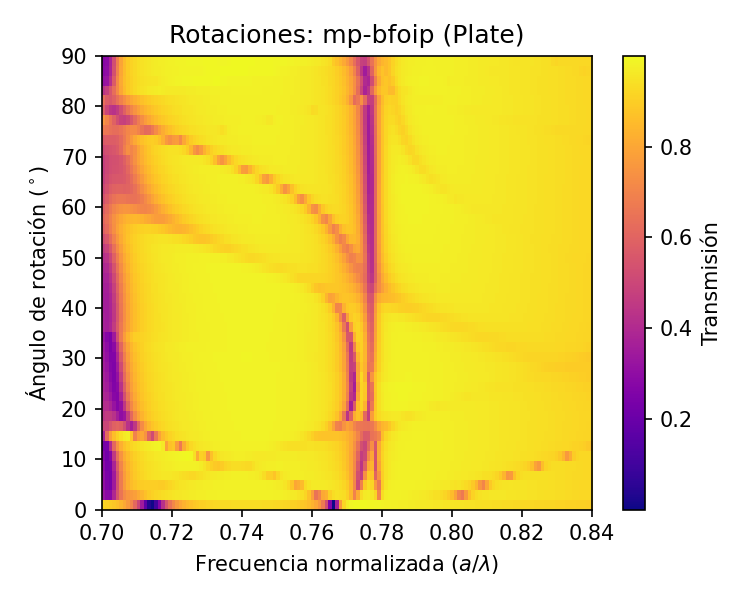
\includegraphics[width=0.48\textwidth]{figures/mp-bfoip_plate_rangle.png}
\hfill
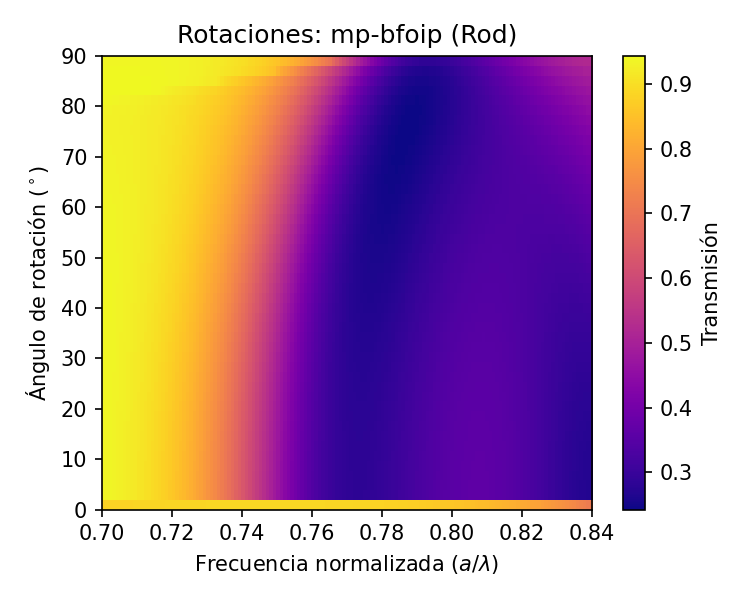
\includegraphics[width=0.48\textwidth]{figures/mp-bfoip_rod_rangle.png}
\caption{Mapas de transmisión por rotación (twist) para mp-bfoip. Izquierda: Lámina. Derecha: Cilindros.}
\end{figure}
\vspace{1em}
\hrule
\vspace{1em}
\subsection*{Material ID: mp-bfojt}
\textbf{Constante Dieléctrica ($\epsilon_{total}$):} 3.90 \\[0.5em]
\begin{table}[h!]
\centering
\begin{tabular}{lcc}
\toprule
\textbf{Métrica} & \textbf{Lámina (Plate)} & \textbf{Cilindros (Rod)} \\
\midrule
Bandgaps ($k_x$) & Ninguno & Ninguno \\
Resonancias ($k_x$) & 36 & 36 \\
\midrule
Bandgaps (Rotación) & Ninguno & Ninguno \\
Resonancias (Rotación) & 33 & 33 \\
\bottomrule
\end{tabular}
\end{table}
\begin{figure}[H]
\centering
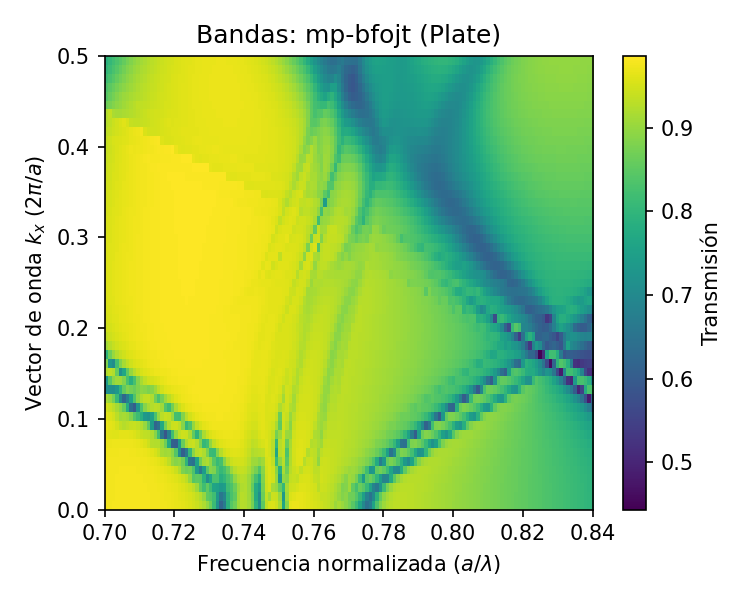
\includegraphics[width=0.48\textwidth]{figures/mp-bfojt_plate.png}
\hfill
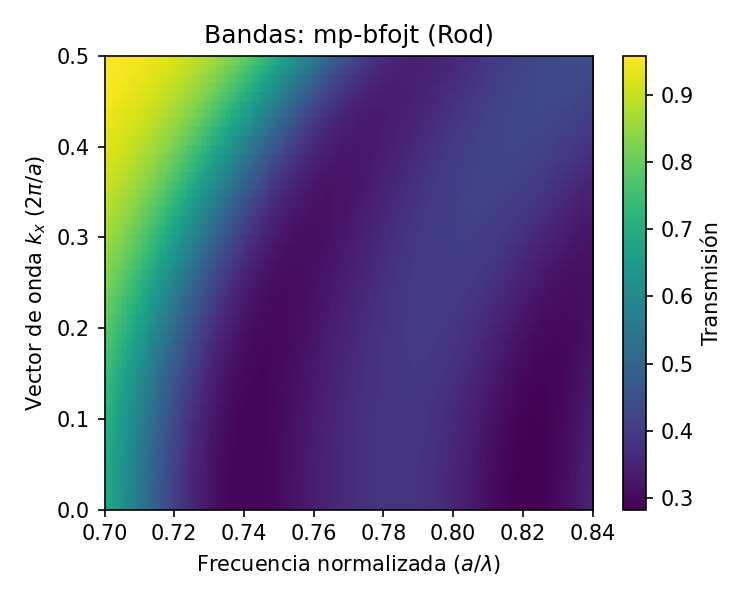
\includegraphics[width=0.48\textwidth]{figures/mp-bfojt_rod.png}
\caption{Estructuras de bandas fotónicas ($k_x$) para mp-bfojt. Izquierda: Lámina. Derecha: Cilindros.}
\end{figure}
\vspace{1em}
\begin{figure}[H]
\centering
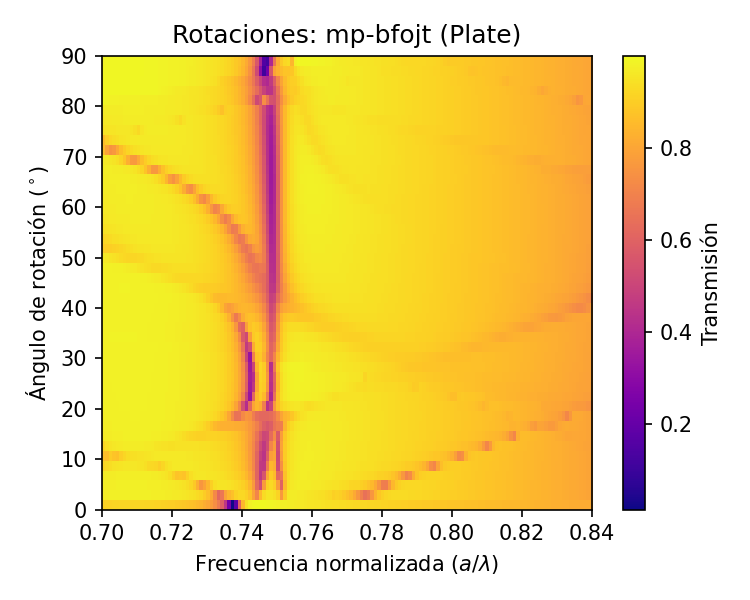
\includegraphics[width=0.48\textwidth]{figures/mp-bfojt_plate_rangle.png}
\hfill
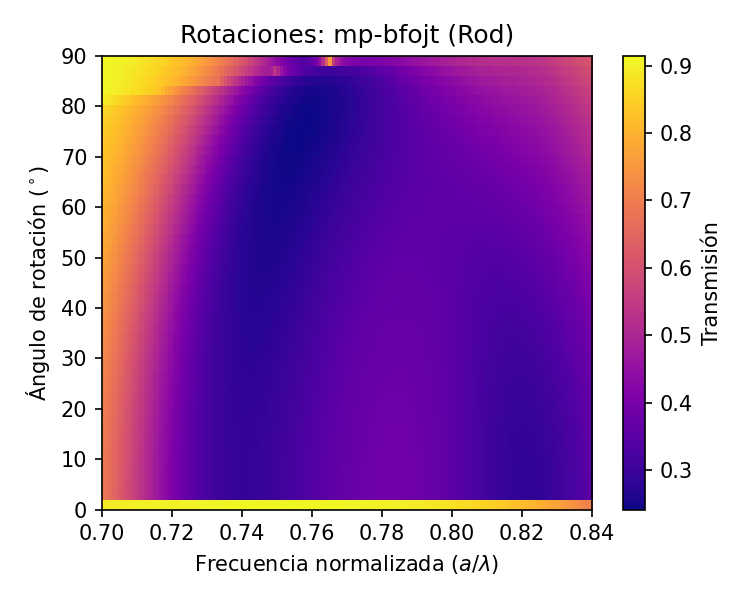
\includegraphics[width=0.48\textwidth]{figures/mp-bfojt_rod_rangle.png}
\caption{Mapas de transmisión por rotación (twist) para mp-bfojt. Izquierda: Lámina. Derecha: Cilindros.}
\end{figure}
\vspace{1em}
\hrule
\vspace{1em}
\subsection*{Material ID: mp-bfpfv}
\textbf{Constante Dieléctrica ($\epsilon_{total}$):} 4.74 \\[0.5em]
\begin{table}[h!]
\centering
\begin{tabular}{lcc}
\toprule
\textbf{Métrica} & \textbf{Lámina (Plate)} & \textbf{Cilindros (Rod)} \\
\midrule
Bandgaps ($k_x$) & Ninguno & Ninguno \\
Resonancias ($k_x$) & 36 & 36 \\
\midrule
Bandgaps (Rotación) & Ninguno & Ninguno \\
Resonancias (Rotación) & 33 & 33 \\
\bottomrule
\end{tabular}
\end{table}
\begin{figure}[H]
\centering
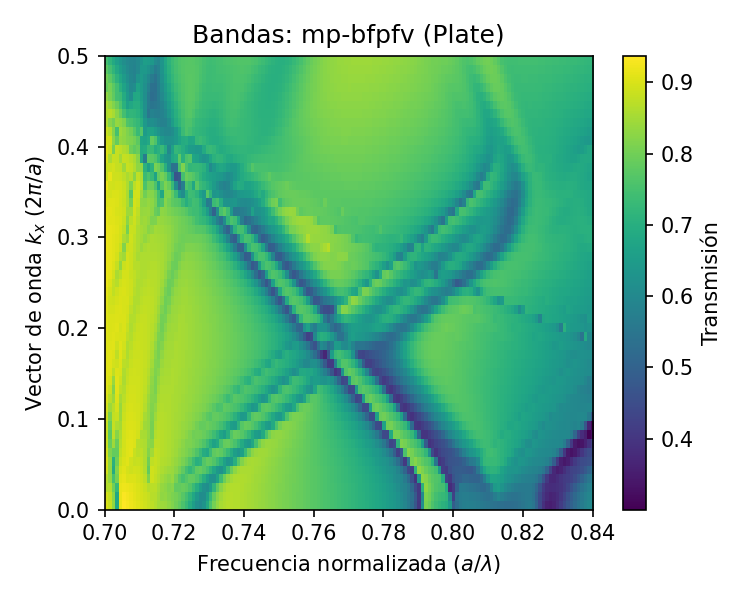
\includegraphics[width=0.48\textwidth]{figures/mp-bfpfv_plate.png}
\hfill
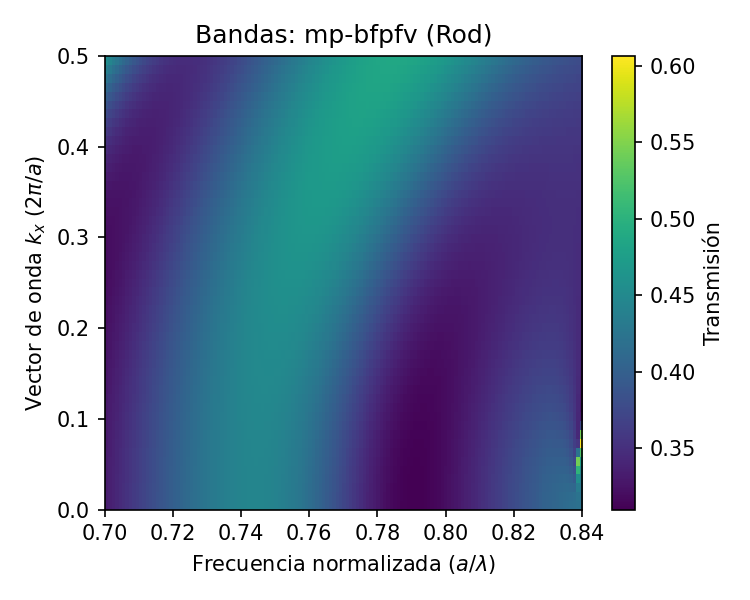
\includegraphics[width=0.48\textwidth]{figures/mp-bfpfv_rod.png}
\caption{Estructuras de bandas fotónicas ($k_x$) para mp-bfpfv. Izquierda: Lámina. Derecha: Cilindros.}
\end{figure}
\vspace{1em}
\begin{figure}[H]
\centering
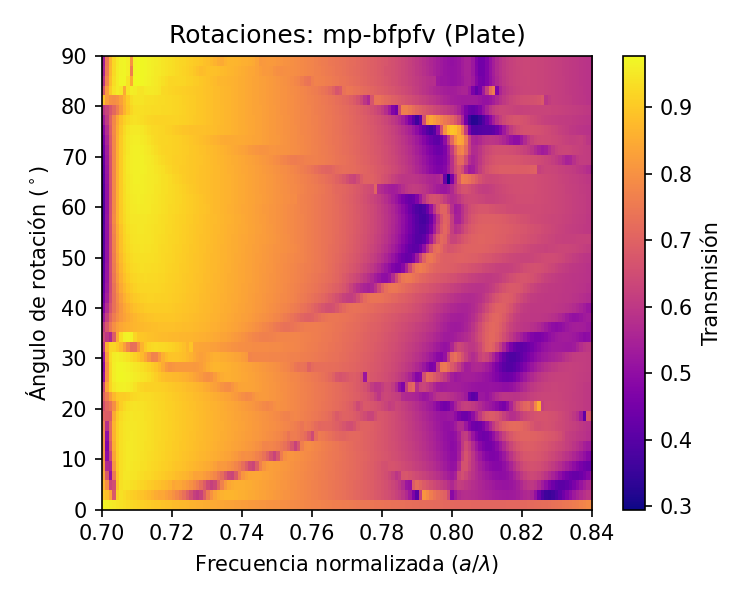
\includegraphics[width=0.48\textwidth]{figures/mp-bfpfv_plate_rangle.png}
\hfill
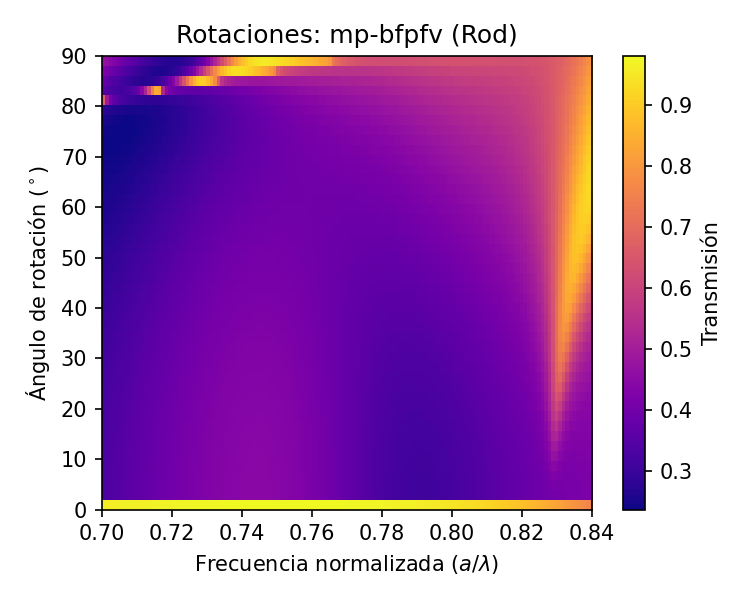
\includegraphics[width=0.48\textwidth]{figures/mp-bfpfv_rod_rangle.png}
\caption{Mapas de transmisión por rotación (twist) para mp-bfpfv. Izquierda: Lámina. Derecha: Cilindros.}
\end{figure}
\vspace{1em}
\hrule
\vspace{1em}
\subsection*{Material ID: mp-bfpjf}
\textbf{Constante Dieléctrica ($\epsilon_{total}$):} 3.90 \\[0.5em]
\begin{table}[h!]
\centering
\begin{tabular}{lcc}
\toprule
\textbf{Métrica} & \textbf{Lámina (Plate)} & \textbf{Cilindros (Rod)} \\
\midrule
Bandgaps ($k_x$) & Ninguno & Ninguno \\
Resonancias ($k_x$) & 36 & 36 \\
\midrule
Bandgaps (Rotación) & Ninguno & Ninguno \\
Resonancias (Rotación) & 33 & 33 \\
\bottomrule
\end{tabular}
\end{table}
\begin{figure}[H]
\centering
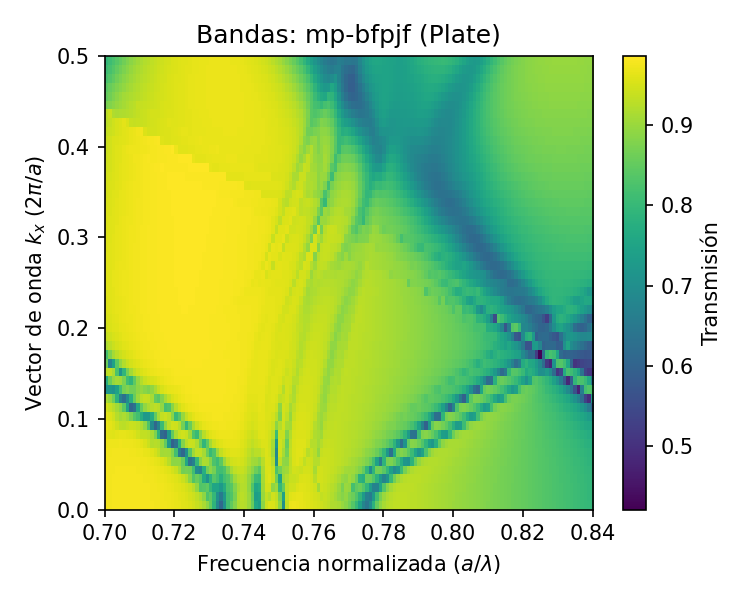
\includegraphics[width=0.48\textwidth]{figures/mp-bfpjf_plate.png}
\hfill
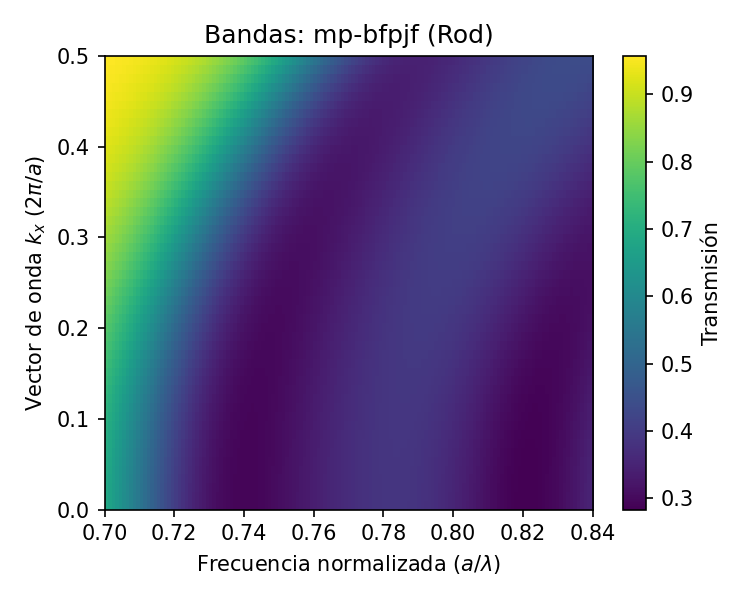
\includegraphics[width=0.48\textwidth]{figures/mp-bfpjf_rod.png}
\caption{Estructuras de bandas fotónicas ($k_x$) para mp-bfpjf. Izquierda: Lámina. Derecha: Cilindros.}
\end{figure}
\vspace{1em}
\begin{figure}[H]
\centering
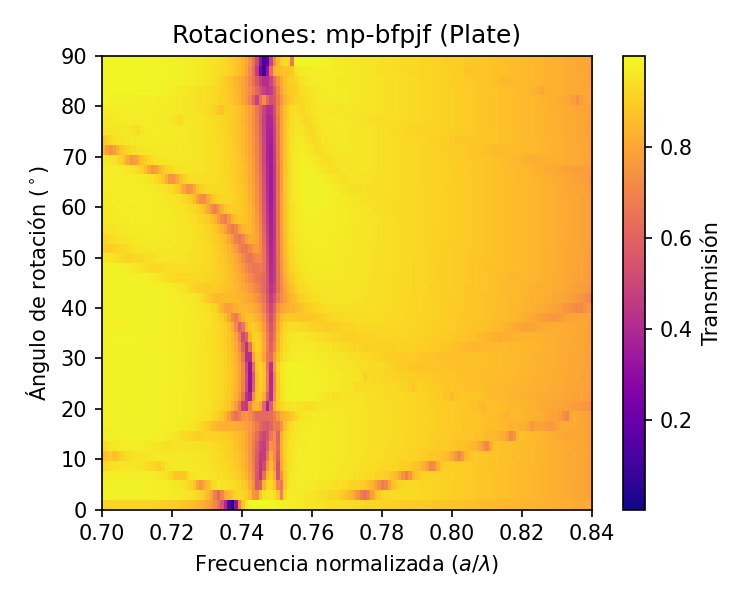
\includegraphics[width=0.48\textwidth]{figures/mp-bfpjf_plate_rangle.png}
\hfill
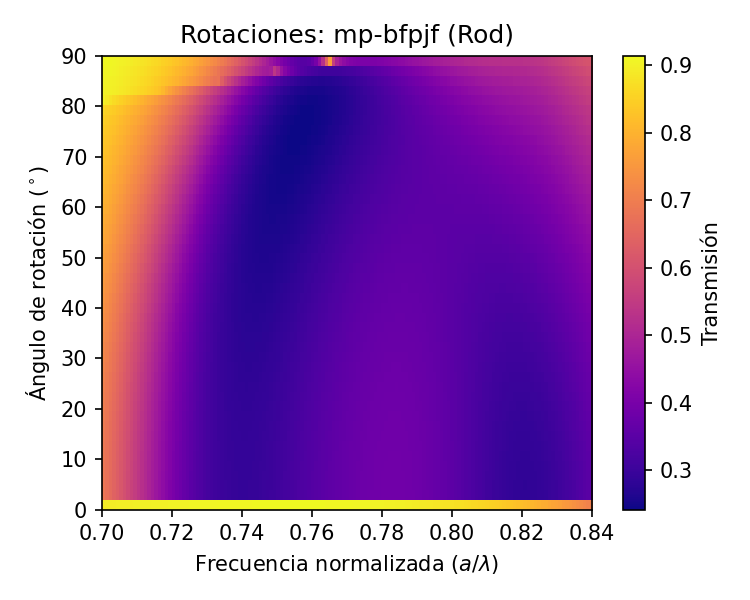
\includegraphics[width=0.48\textwidth]{figures/mp-bfpjf_rod_rangle.png}
\caption{Mapas de transmisión por rotación (twist) para mp-bfpjf. Izquierda: Lámina. Derecha: Cilindros.}
\end{figure}
\vspace{1em}
\hrule
\vspace{1em}
\subsection*{Material ID: mp-bfpjv}
\textbf{Constante Dieléctrica ($\epsilon_{total}$):} 3.38 \\[0.5em]
\begin{table}[h!]
\centering
\begin{tabular}{lcc}
\toprule
\textbf{Métrica} & \textbf{Lámina (Plate)} & \textbf{Cilindros (Rod)} \\
\midrule
Bandgaps ($k_x$) & Ninguno & Ninguno \\
Resonancias ($k_x$) & 36 & 36 \\
\midrule
Bandgaps (Rotación) & Ninguno & Ninguno \\
Resonancias (Rotación) & 33 & 33 \\
\bottomrule
\end{tabular}
\end{table}
\begin{figure}[H]
\centering
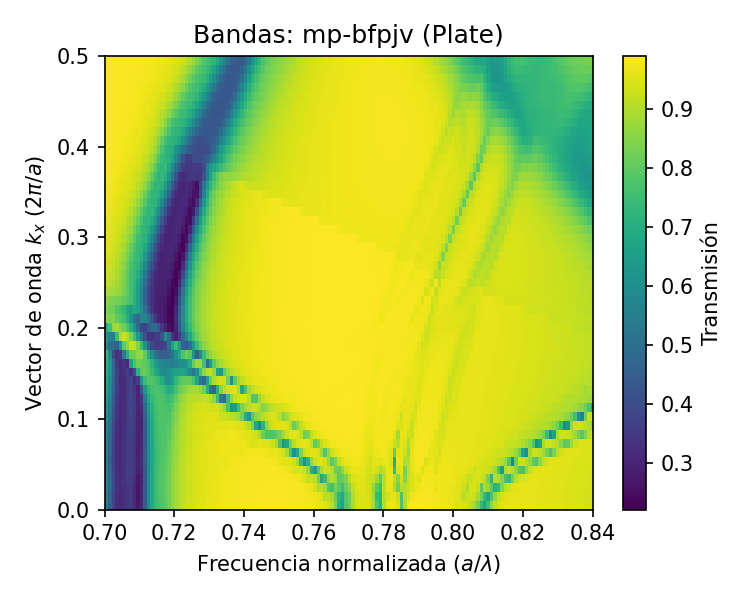
\includegraphics[width=0.48\textwidth]{figures/mp-bfpjv_plate.png}
\hfill
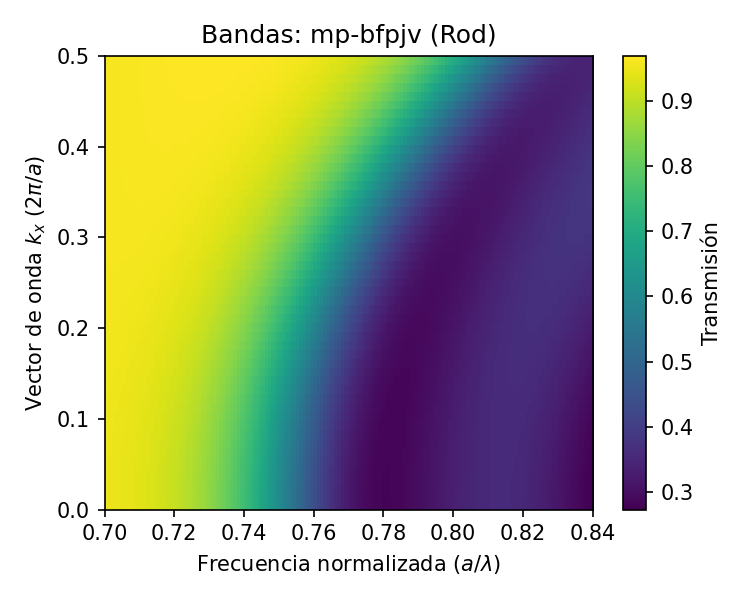
\includegraphics[width=0.48\textwidth]{figures/mp-bfpjv_rod.png}
\caption{Estructuras de bandas fotónicas ($k_x$) para mp-bfpjv. Izquierda: Lámina. Derecha: Cilindros.}
\end{figure}
\vspace{1em}
\begin{figure}[H]
\centering
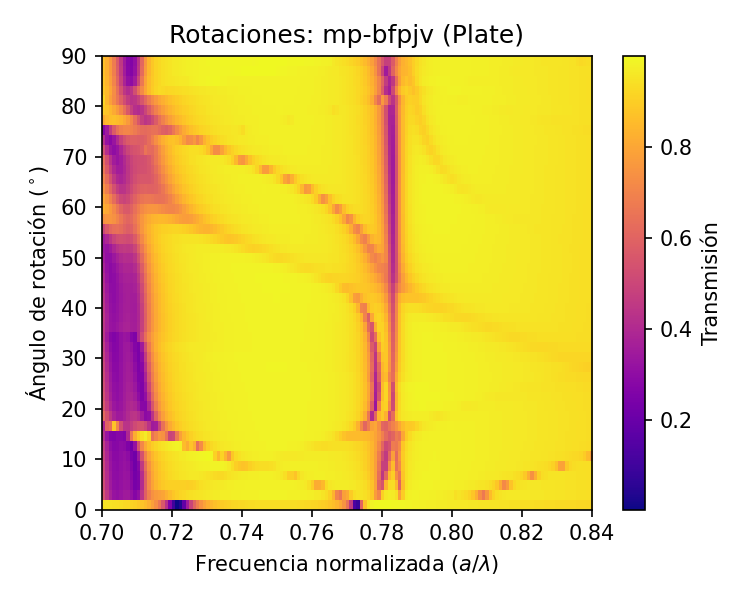
\includegraphics[width=0.48\textwidth]{figures/mp-bfpjv_plate_rangle.png}
\hfill
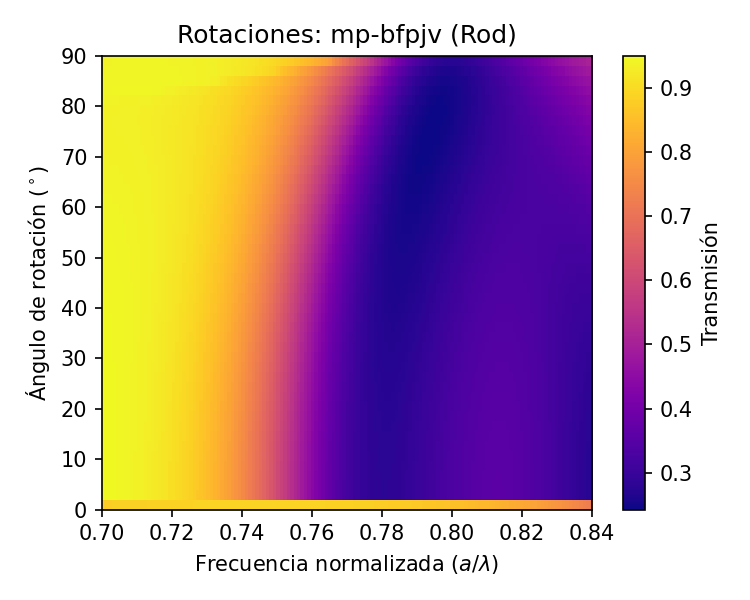
\includegraphics[width=0.48\textwidth]{figures/mp-bfpjv_rod_rangle.png}
\caption{Mapas de transmisión por rotación (twist) para mp-bfpjv. Izquierda: Lámina. Derecha: Cilindros.}
\end{figure}
\vspace{1em}
\hrule
\vspace{1em}
\subsection*{Material ID: mp-bfqil}
\textbf{Constante Dieléctrica ($\epsilon_{total}$):} 3.88 \\[0.5em]
\begin{table}[h!]
\centering
\begin{tabular}{lcc}
\toprule
\textbf{Métrica} & \textbf{Lámina (Plate)} & \textbf{Cilindros (Rod)} \\
\midrule
Bandgaps ($k_x$) & Ninguno & Ninguno \\
Resonancias ($k_x$) & 36 & 36 \\
\midrule
Bandgaps (Rotación) & Ninguno & Ninguno \\
Resonancias (Rotación) & 33 & 33 \\
\bottomrule
\end{tabular}
\end{table}
\begin{figure}[H]
\centering
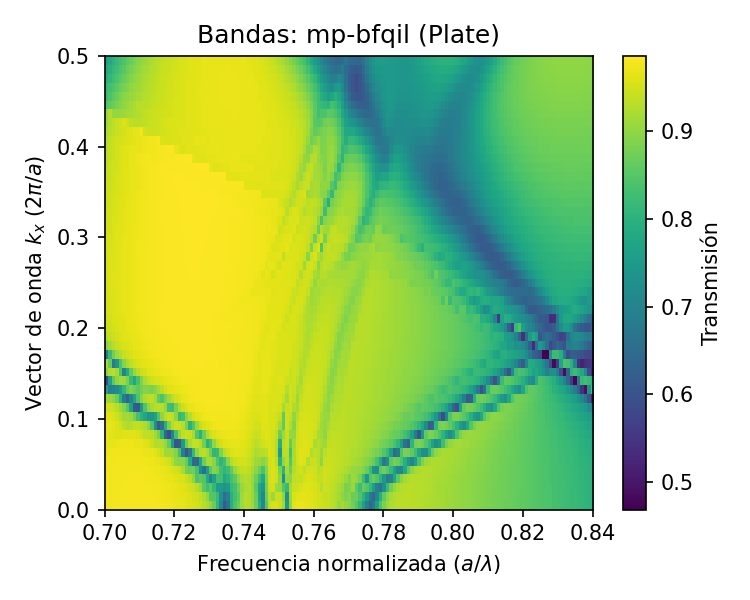
\includegraphics[width=0.48\textwidth]{figures/mp-bfqil_plate.png}
\hfill
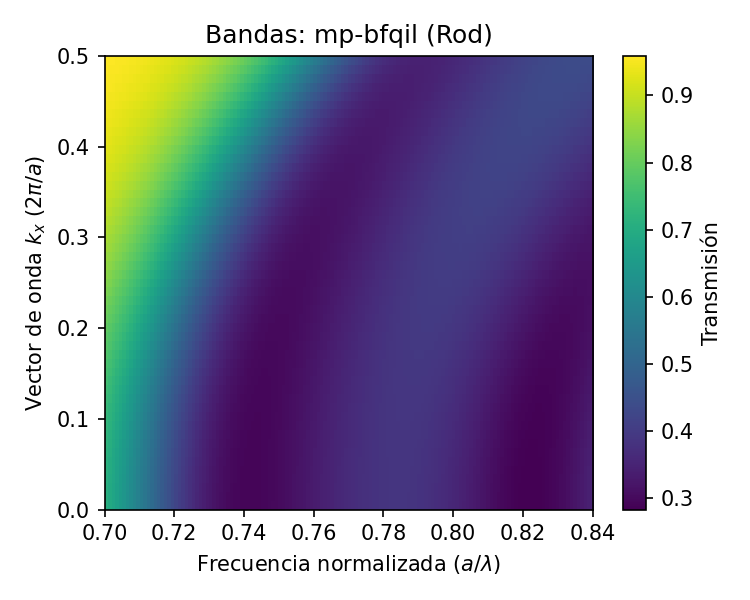
\includegraphics[width=0.48\textwidth]{figures/mp-bfqil_rod.png}
\caption{Estructuras de bandas fotónicas ($k_x$) para mp-bfqil. Izquierda: Lámina. Derecha: Cilindros.}
\end{figure}
\vspace{1em}
\begin{figure}[H]
\centering
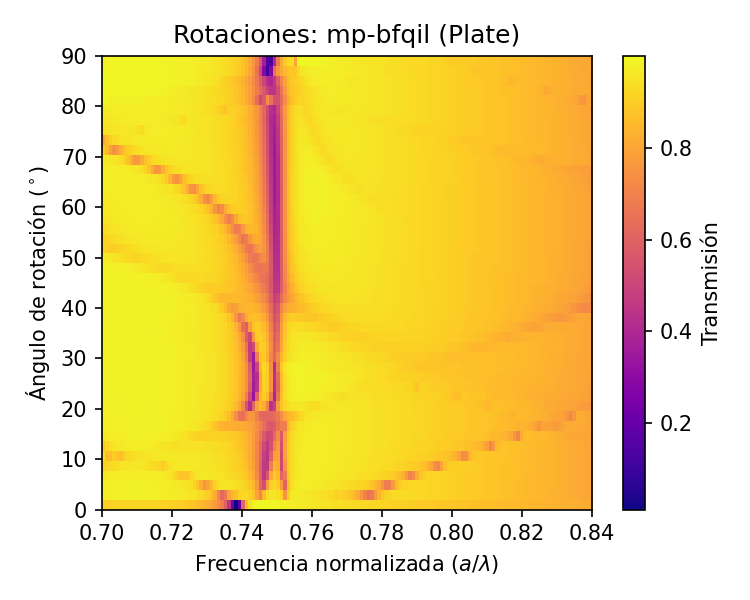
\includegraphics[width=0.48\textwidth]{figures/mp-bfqil_plate_rangle.png}
\hfill
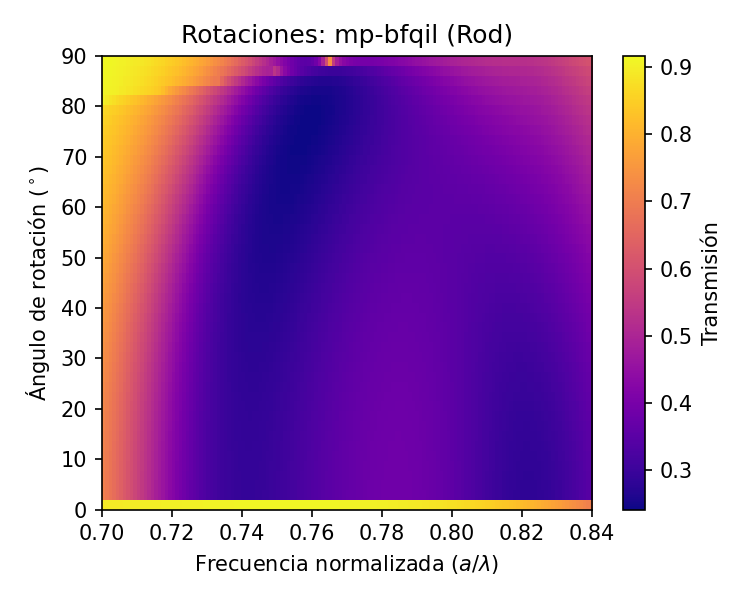
\includegraphics[width=0.48\textwidth]{figures/mp-bfqil_rod_rangle.png}
\caption{Mapas de transmisión por rotación (twist) para mp-bfqil. Izquierda: Lámina. Derecha: Cilindros.}
\end{figure}
\vspace{1em}
\hrule
\vspace{1em}
\subsection*{Material ID: mp-bfqva}
\textbf{Constante Dieléctrica ($\epsilon_{total}$):} 3.51 \\[0.5em]
\begin{table}[h!]
\centering
\begin{tabular}{lcc}
\toprule
\textbf{Métrica} & \textbf{Lámina (Plate)} & \textbf{Cilindros (Rod)} \\
\midrule
Bandgaps ($k_x$) & Ninguno & Ninguno \\
Resonancias ($k_x$) & 36 & 36 \\
\midrule
Bandgaps (Rotación) & Ninguno & Ninguno \\
Resonancias (Rotación) & 33 & 33 \\
\bottomrule
\end{tabular}
\end{table}
\begin{figure}[H]
\centering
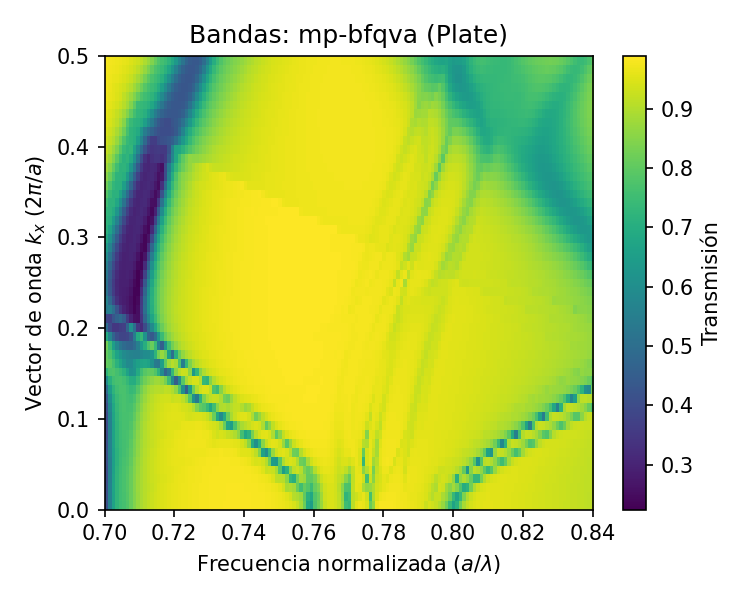
\includegraphics[width=0.48\textwidth]{figures/mp-bfqva_plate.png}
\hfill
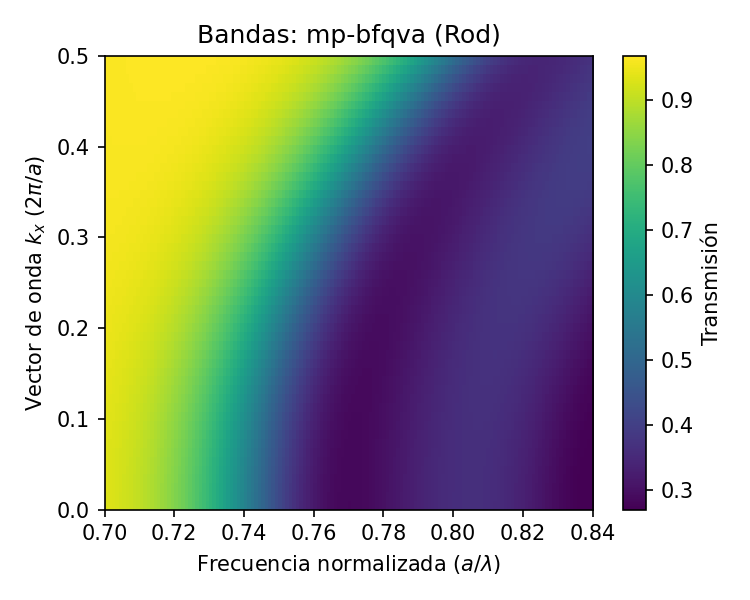
\includegraphics[width=0.48\textwidth]{figures/mp-bfqva_rod.png}
\caption{Estructuras de bandas fotónicas ($k_x$) para mp-bfqva. Izquierda: Lámina. Derecha: Cilindros.}
\end{figure}
\vspace{1em}
\begin{figure}[H]
\centering
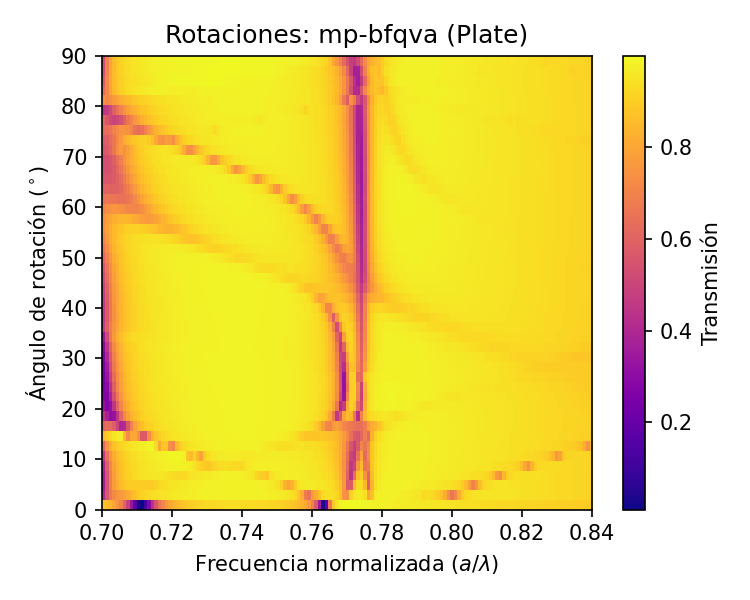
\includegraphics[width=0.48\textwidth]{figures/mp-bfqva_plate_rangle.png}
\hfill
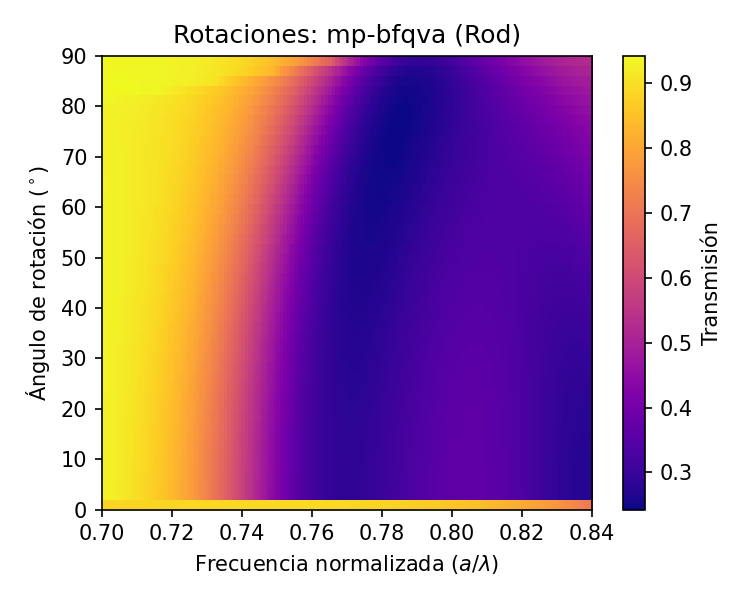
\includegraphics[width=0.48\textwidth]{figures/mp-bfqva_rod_rangle.png}
\caption{Mapas de transmisión por rotación (twist) para mp-bfqva. Izquierda: Lámina. Derecha: Cilindros.}
\end{figure}
\vspace{1em}
\hrule
\vspace{1em}
\subsection*{Material ID: mp-bfqyx}
\textbf{Constante Dieléctrica ($\epsilon_{total}$):} 4.31 \\[0.5em]
\begin{table}[h!]
\centering
\begin{tabular}{lcc}
\toprule
\textbf{Métrica} & \textbf{Lámina (Plate)} & \textbf{Cilindros (Rod)} \\
\midrule
Bandgaps ($k_x$) & Ninguno & Ninguno \\
Resonancias ($k_x$) & 36 & 36 \\
\midrule
Bandgaps (Rotación) & Ninguno & Ninguno \\
Resonancias (Rotación) & 33 & 33 \\
\bottomrule
\end{tabular}
\end{table}
\begin{figure}[H]
\centering
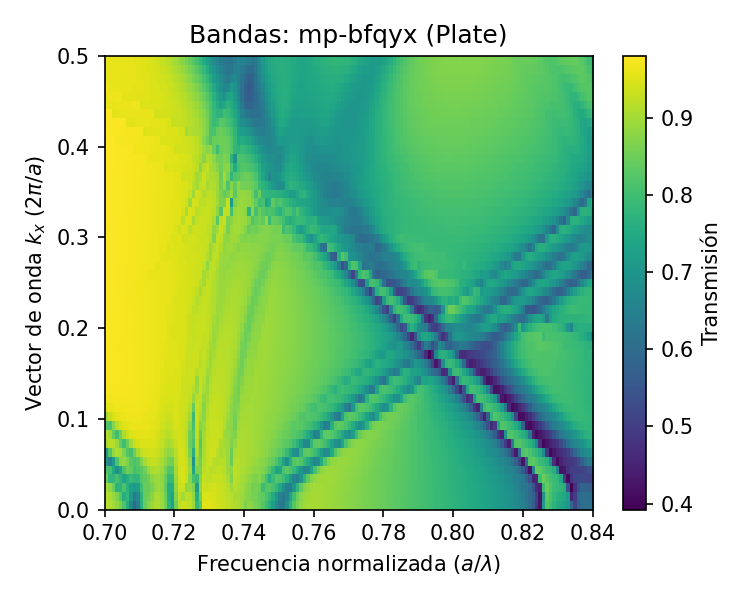
\includegraphics[width=0.48\textwidth]{figures/mp-bfqyx_plate.png}
\hfill
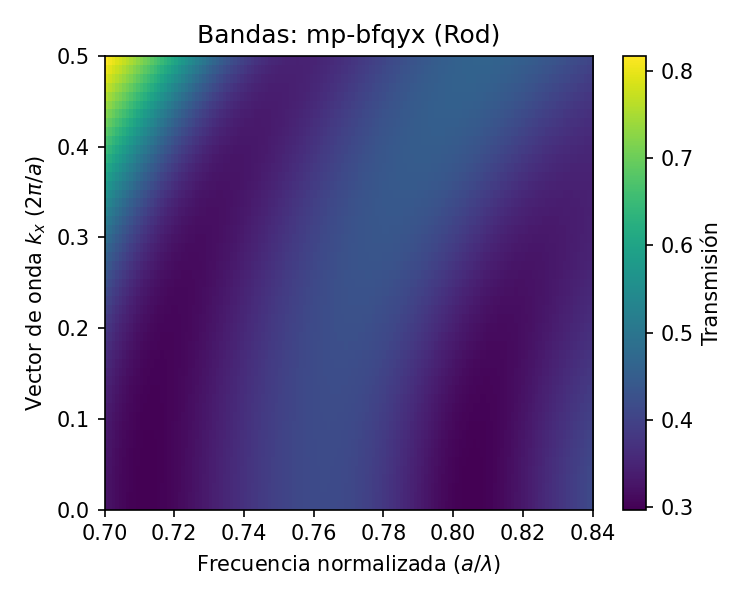
\includegraphics[width=0.48\textwidth]{figures/mp-bfqyx_rod.png}
\caption{Estructuras de bandas fotónicas ($k_x$) para mp-bfqyx. Izquierda: Lámina. Derecha: Cilindros.}
\end{figure}
\vspace{1em}
\begin{figure}[H]
\centering
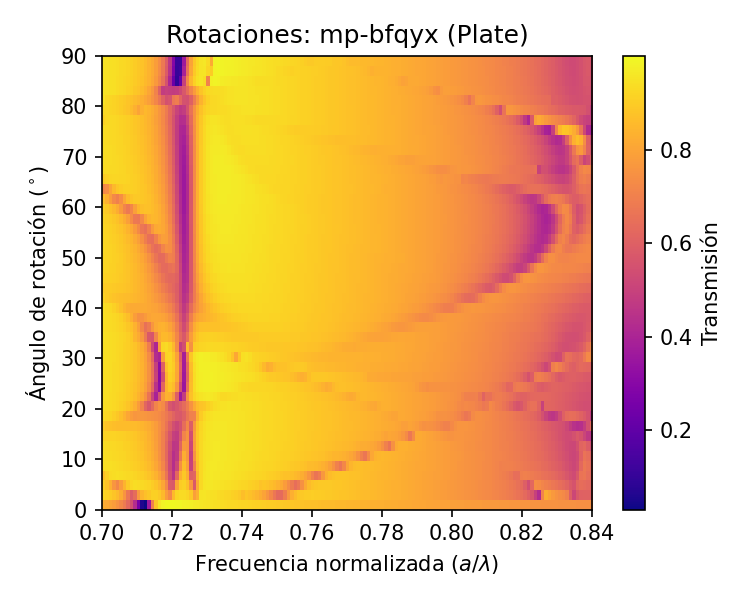
\includegraphics[width=0.48\textwidth]{figures/mp-bfqyx_plate_rangle.png}
\hfill
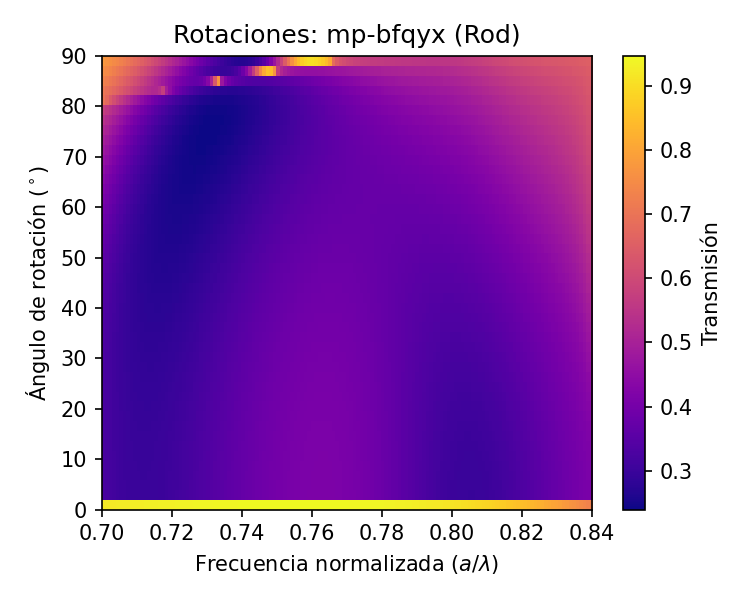
\includegraphics[width=0.48\textwidth]{figures/mp-bfqyx_rod_rangle.png}
\caption{Mapas de transmisión por rotación (twist) para mp-bfqyx. Izquierda: Lámina. Derecha: Cilindros.}
\end{figure}
\vspace{1em}
\hrule
\vspace{1em}
\subsection*{Material ID: mp-bfrhx}
\textbf{Constante Dieléctrica ($\epsilon_{total}$):} 4.71 \\[0.5em]
\begin{table}[h!]
\centering
\begin{tabular}{lcc}
\toprule
\textbf{Métrica} & \textbf{Lámina (Plate)} & \textbf{Cilindros (Rod)} \\
\midrule
Bandgaps ($k_x$) & Ninguno & Ninguno \\
Resonancias ($k_x$) & 36 & 36 \\
\midrule
Bandgaps (Rotación) & Ninguno & Ninguno \\
Resonancias (Rotación) & 33 & 33 \\
\bottomrule
\end{tabular}
\end{table}
\begin{figure}[H]
\centering
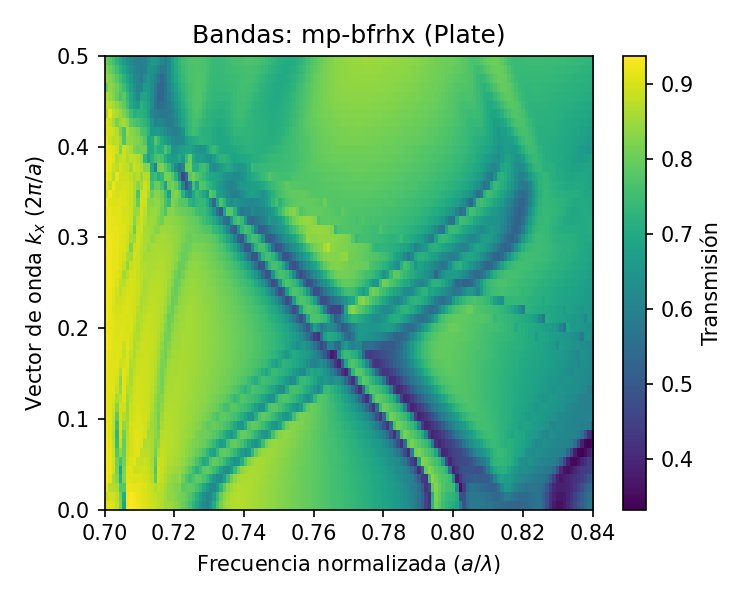
\includegraphics[width=0.48\textwidth]{figures/mp-bfrhx_plate.png}
\hfill
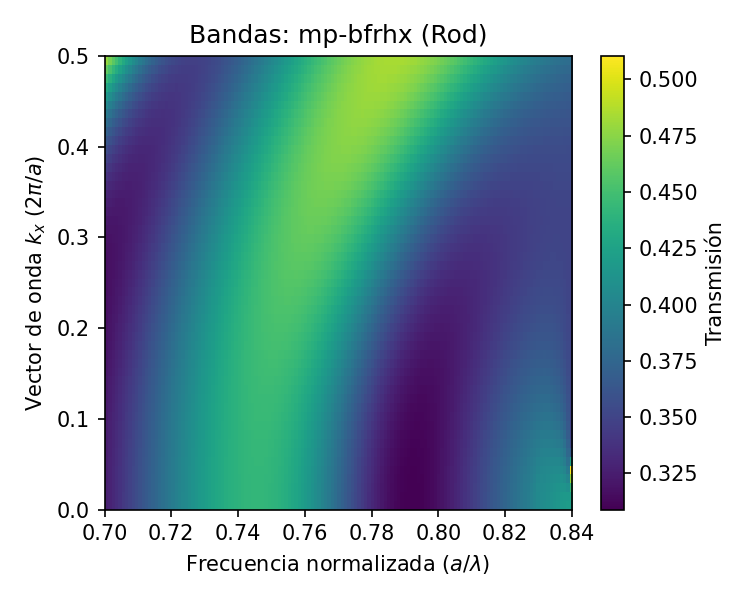
\includegraphics[width=0.48\textwidth]{figures/mp-bfrhx_rod.png}
\caption{Estructuras de bandas fotónicas ($k_x$) para mp-bfrhx. Izquierda: Lámina. Derecha: Cilindros.}
\end{figure}
\vspace{1em}
\begin{figure}[H]
\centering
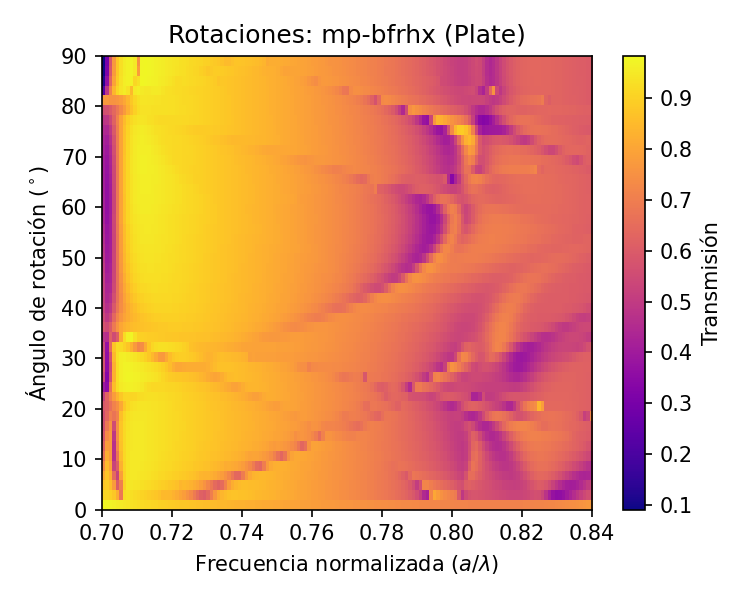
\includegraphics[width=0.48\textwidth]{figures/mp-bfrhx_plate_rangle.png}
\hfill
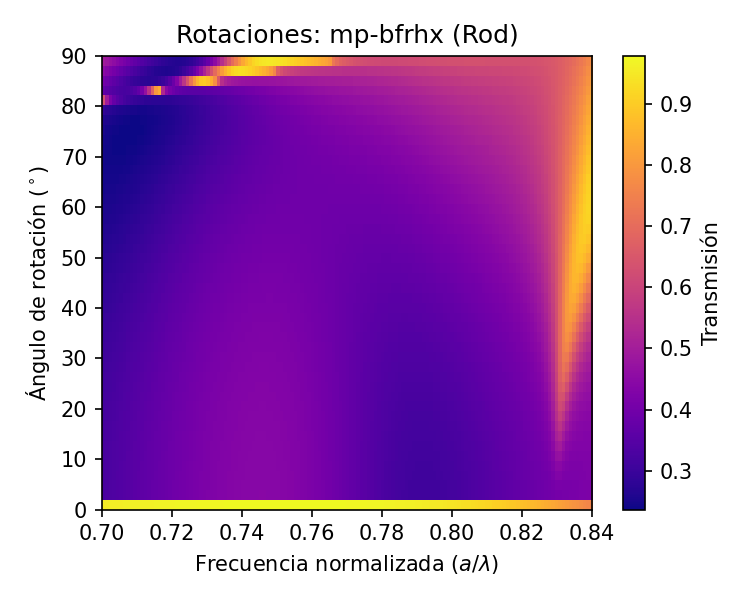
\includegraphics[width=0.48\textwidth]{figures/mp-bfrhx_rod_rangle.png}
\caption{Mapas de transmisión por rotación (twist) para mp-bfrhx. Izquierda: Lámina. Derecha: Cilindros.}
\end{figure}
\vspace{1em}
\hrule
\vspace{1em}
\subsection*{Material ID: mp-bfrjg}
\textbf{Constante Dieléctrica ($\epsilon_{total}$):} 6.32 \\[0.5em]
\begin{table}[h!]
\centering
\begin{tabular}{lcc}
\toprule
\textbf{Métrica} & \textbf{Lámina (Plate)} & \textbf{Cilindros (Rod)} \\
\midrule
Bandgaps ($k_x$) & Ninguno & Ninguno \\
Resonancias ($k_x$) & 36 & 36 \\
\midrule
Bandgaps (Rotación) & Ninguno & Ninguno \\
Resonancias (Rotación) & 33 & 33 \\
\bottomrule
\end{tabular}
\end{table}
\begin{figure}[H]
\centering
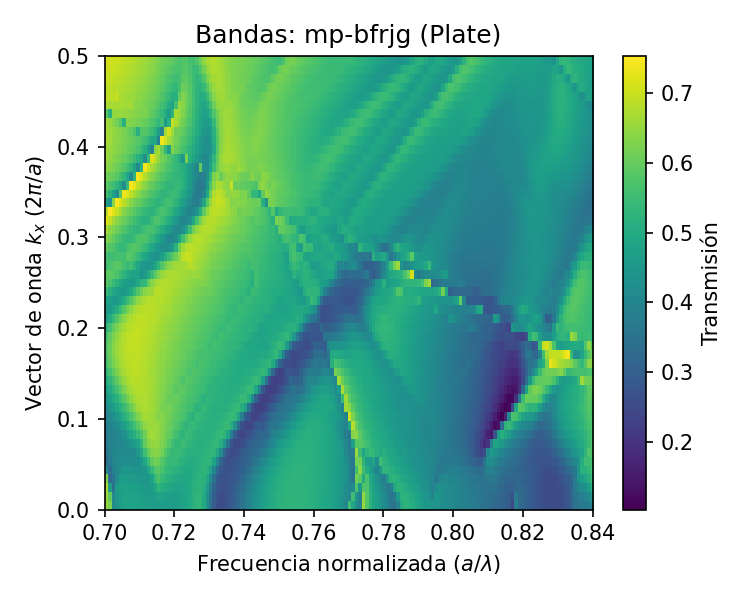
\includegraphics[width=0.48\textwidth]{figures/mp-bfrjg_plate.png}
\hfill
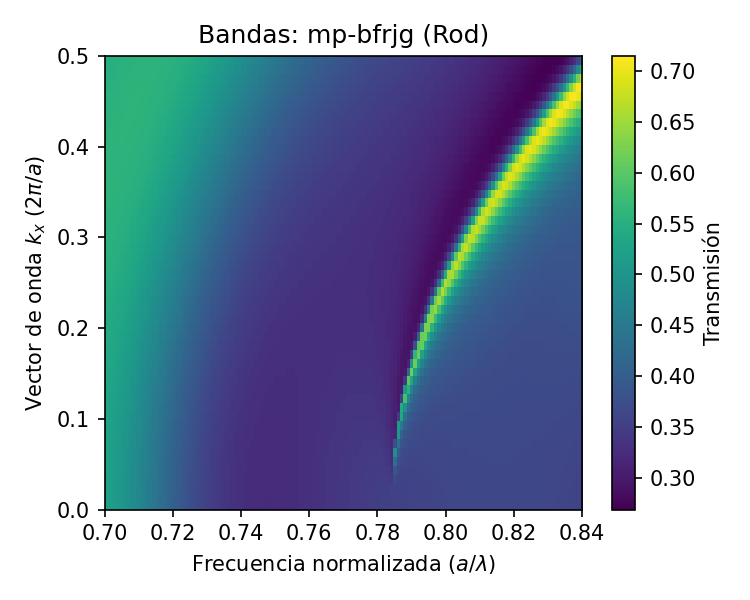
\includegraphics[width=0.48\textwidth]{figures/mp-bfrjg_rod.png}
\caption{Estructuras de bandas fotónicas ($k_x$) para mp-bfrjg. Izquierda: Lámina. Derecha: Cilindros.}
\end{figure}
\vspace{1em}
\begin{figure}[H]
\centering
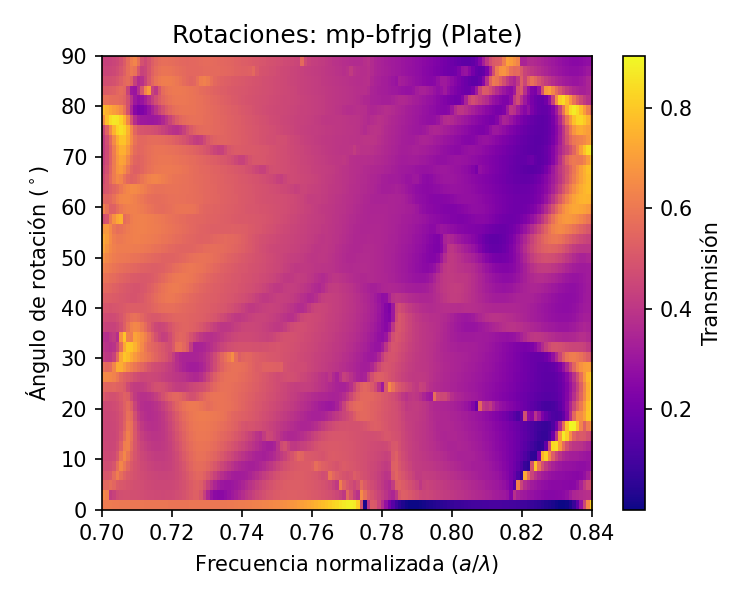
\includegraphics[width=0.48\textwidth]{figures/mp-bfrjg_plate_rangle.png}
\hfill
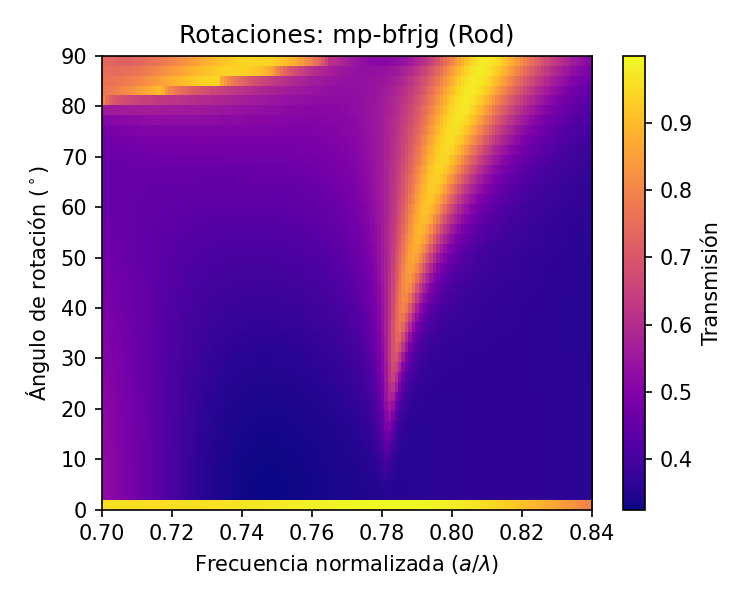
\includegraphics[width=0.48\textwidth]{figures/mp-bfrjg_rod_rangle.png}
\caption{Mapas de transmisión por rotación (twist) para mp-bfrjg. Izquierda: Lámina. Derecha: Cilindros.}
\end{figure}
\vspace{1em}
\hrule
\vspace{1em}
\subsection*{Material ID: mp-bfrqy}
\textbf{Constante Dieléctrica ($\epsilon_{total}$):} 4.78 \\[0.5em]
\begin{table}[h!]
\centering
\begin{tabular}{lcc}
\toprule
\textbf{Métrica} & \textbf{Lámina (Plate)} & \textbf{Cilindros (Rod)} \\
\midrule
Bandgaps ($k_x$) & Ninguno & Ninguno \\
Resonancias ($k_x$) & 36 & 36 \\
\midrule
Bandgaps (Rotación) & Ninguno & Ninguno \\
Resonancias (Rotación) & 33 & 33 \\
\bottomrule
\end{tabular}
\end{table}
\begin{figure}[H]
\centering
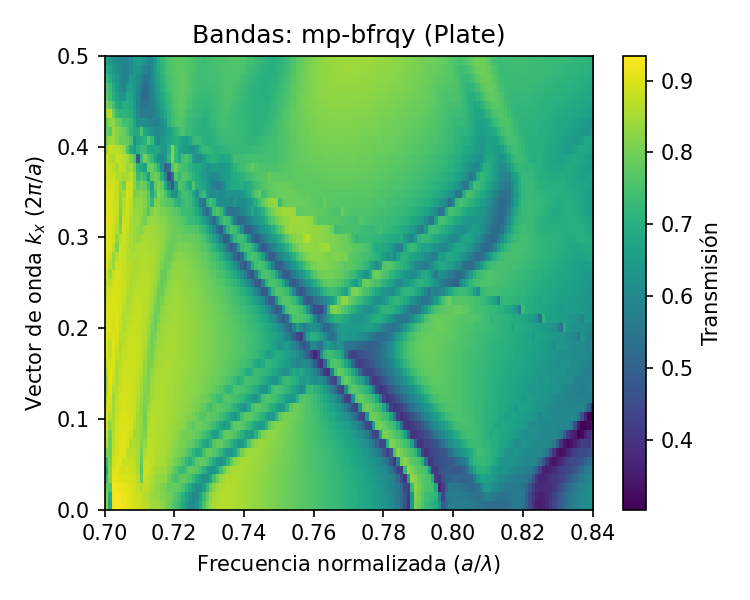
\includegraphics[width=0.48\textwidth]{figures/mp-bfrqy_plate.png}
\hfill
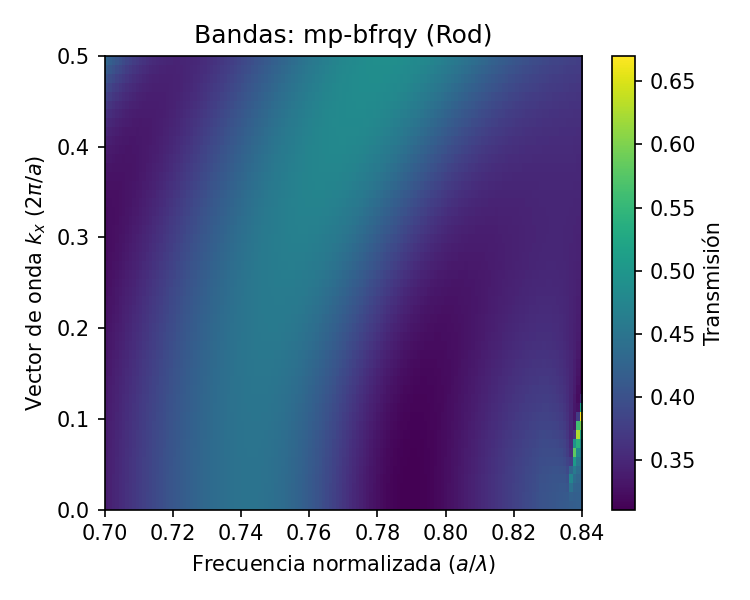
\includegraphics[width=0.48\textwidth]{figures/mp-bfrqy_rod.png}
\caption{Estructuras de bandas fotónicas ($k_x$) para mp-bfrqy. Izquierda: Lámina. Derecha: Cilindros.}
\end{figure}
\vspace{1em}
\begin{figure}[H]
\centering
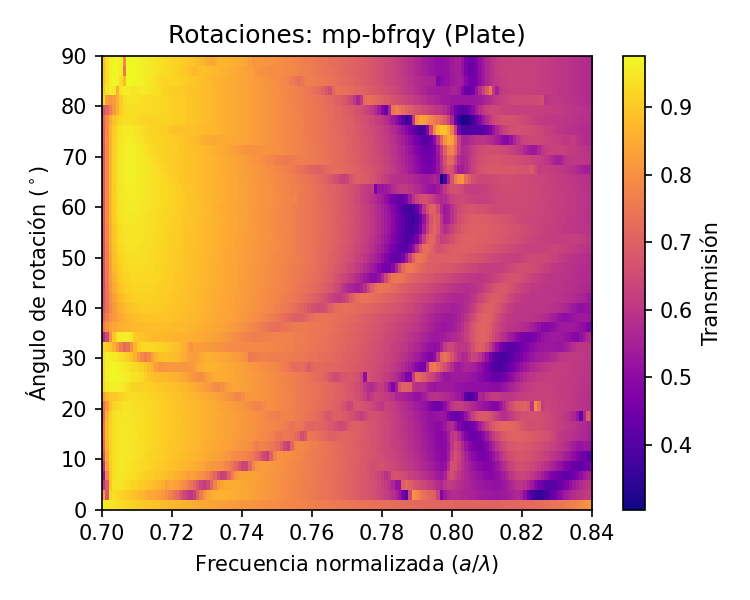
\includegraphics[width=0.48\textwidth]{figures/mp-bfrqy_plate_rangle.png}
\hfill
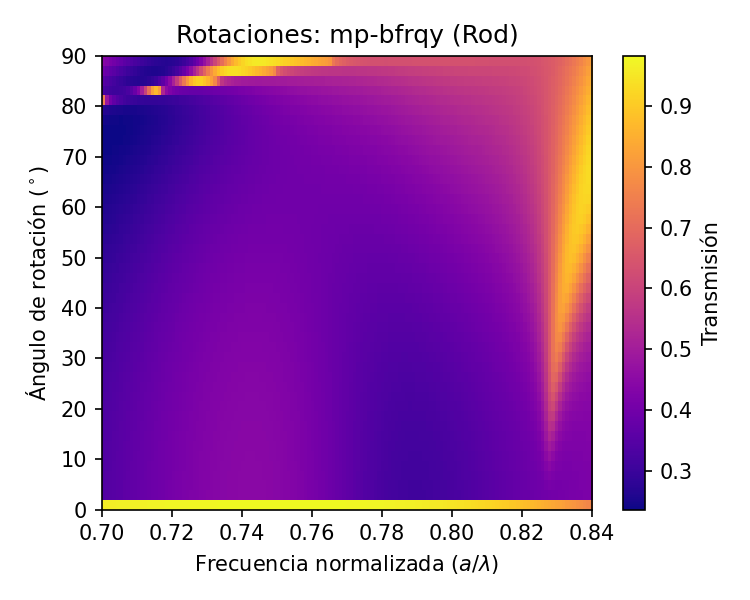
\includegraphics[width=0.48\textwidth]{figures/mp-bfrqy_rod_rangle.png}
\caption{Mapas de transmisión por rotación (twist) para mp-bfrqy. Izquierda: Lámina. Derecha: Cilindros.}
\end{figure}
\vspace{1em}
\hrule
\vspace{1em}
\subsection*{Material ID: mp-bfrum}
\textbf{Constante Dieléctrica ($\epsilon_{total}$):} 4.25 \\[0.5em]
\begin{table}[h!]
\centering
\begin{tabular}{lcc}
\toprule
\textbf{Métrica} & \textbf{Lámina (Plate)} & \textbf{Cilindros (Rod)} \\
\midrule
Bandgaps ($k_x$) & Ninguno & Ninguno \\
Resonancias ($k_x$) & 36 & 36 \\
\midrule
Bandgaps (Rotación) & Ninguno & Ninguno \\
Resonancias (Rotación) & 33 & 33 \\
\bottomrule
\end{tabular}
\end{table}
\begin{figure}[H]
\centering
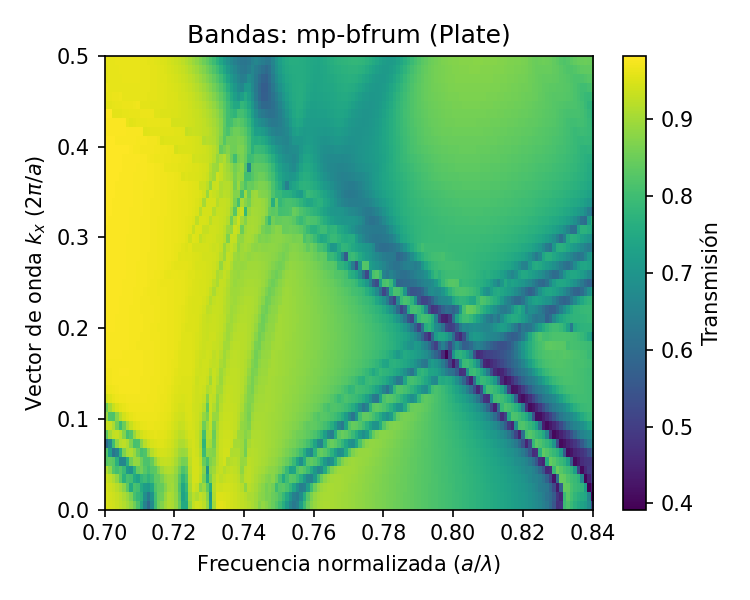
\includegraphics[width=0.48\textwidth]{figures/mp-bfrum_plate.png}
\hfill
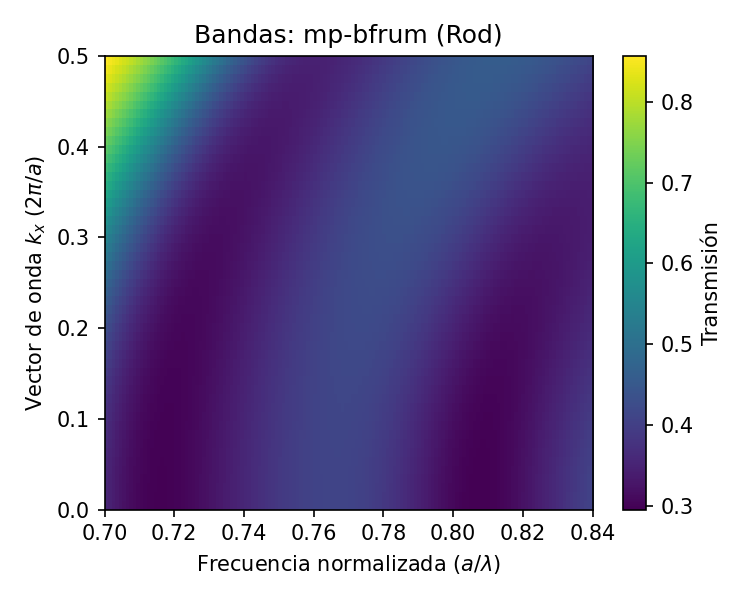
\includegraphics[width=0.48\textwidth]{figures/mp-bfrum_rod.png}
\caption{Estructuras de bandas fotónicas ($k_x$) para mp-bfrum. Izquierda: Lámina. Derecha: Cilindros.}
\end{figure}
\vspace{1em}
\begin{figure}[H]
\centering
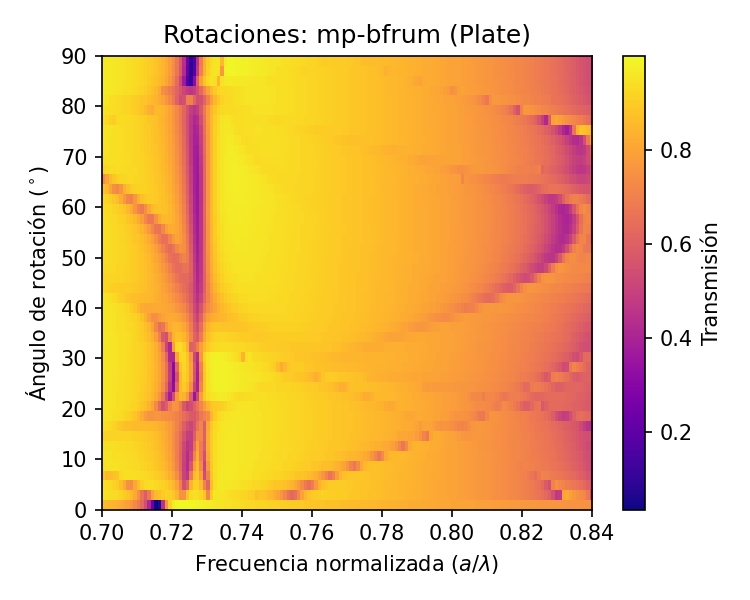
\includegraphics[width=0.48\textwidth]{figures/mp-bfrum_plate_rangle.png}
\hfill
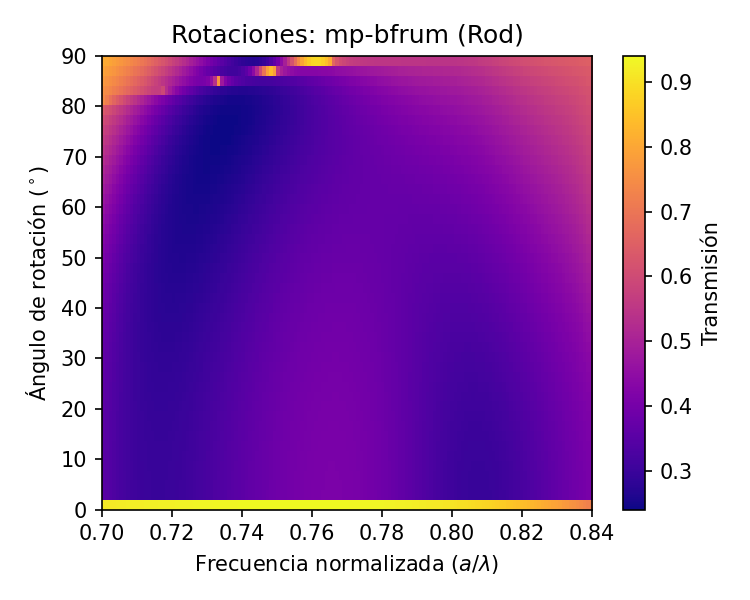
\includegraphics[width=0.48\textwidth]{figures/mp-bfrum_rod_rangle.png}
\caption{Mapas de transmisión por rotación (twist) para mp-bfrum. Izquierda: Lámina. Derecha: Cilindros.}
\end{figure}
\vspace{1em}
\hrule
\vspace{1em}
\subsection*{Material ID: mp-bfrxp}
\textbf{Constante Dieléctrica ($\epsilon_{total}$):} 3.89 \\[0.5em]
\begin{table}[h!]
\centering
\begin{tabular}{lcc}
\toprule
\textbf{Métrica} & \textbf{Lámina (Plate)} & \textbf{Cilindros (Rod)} \\
\midrule
Bandgaps ($k_x$) & Ninguno & Ninguno \\
Resonancias ($k_x$) & 36 & 36 \\
\midrule
Bandgaps (Rotación) & Ninguno & Ninguno \\
Resonancias (Rotación) & 33 & 33 \\
\bottomrule
\end{tabular}
\end{table}
\begin{figure}[H]
\centering
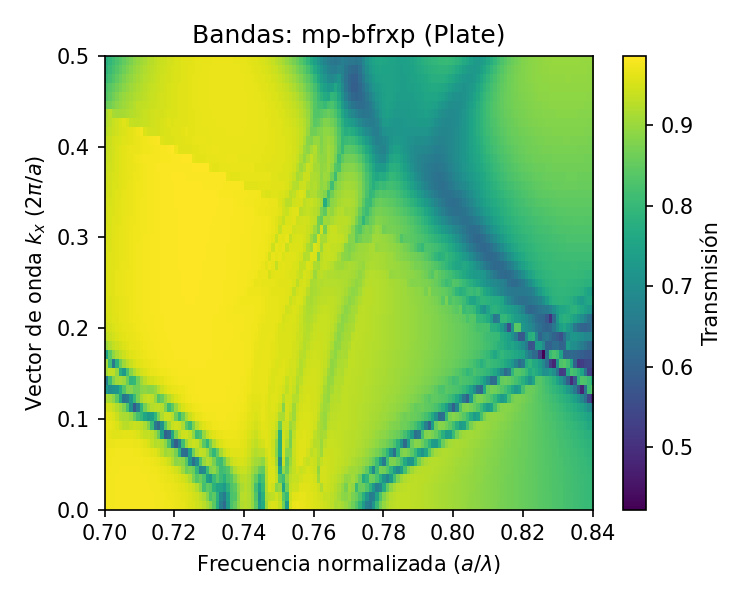
\includegraphics[width=0.48\textwidth]{figures/mp-bfrxp_plate.png}
\hfill
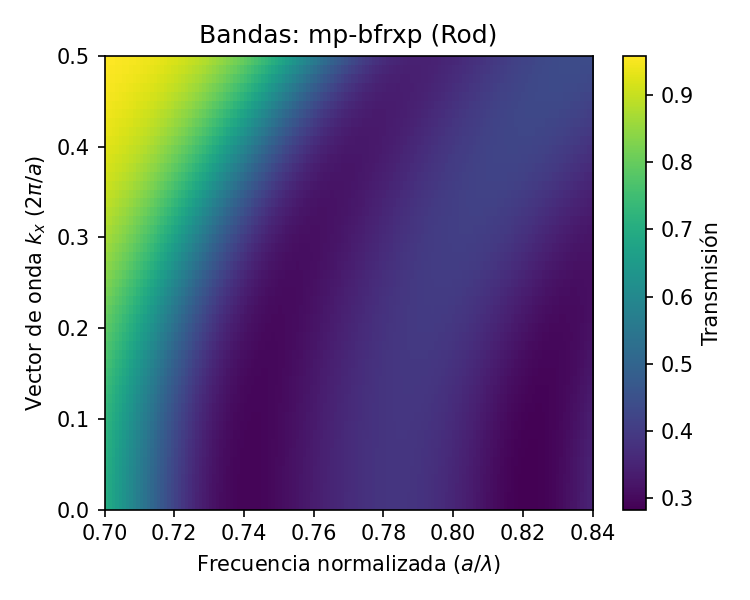
\includegraphics[width=0.48\textwidth]{figures/mp-bfrxp_rod.png}
\caption{Estructuras de bandas fotónicas ($k_x$) para mp-bfrxp. Izquierda: Lámina. Derecha: Cilindros.}
\end{figure}
\vspace{1em}
\begin{figure}[H]
\centering
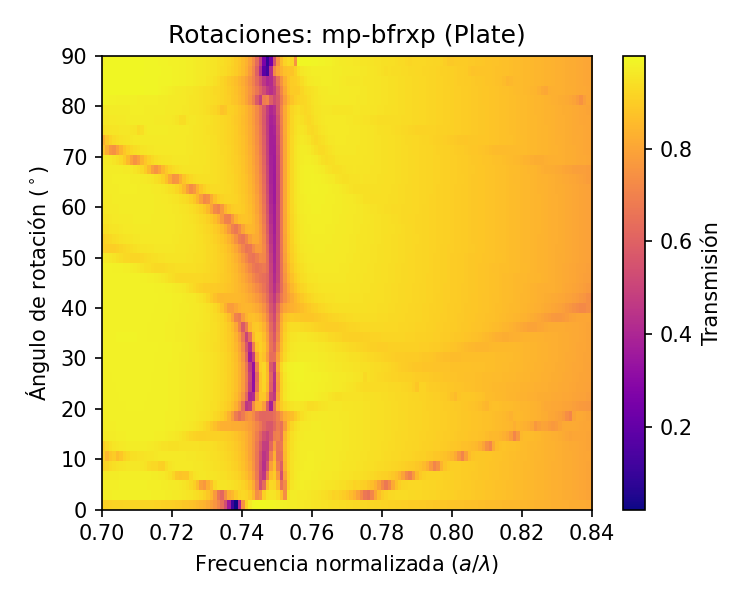
\includegraphics[width=0.48\textwidth]{figures/mp-bfrxp_plate_rangle.png}
\hfill
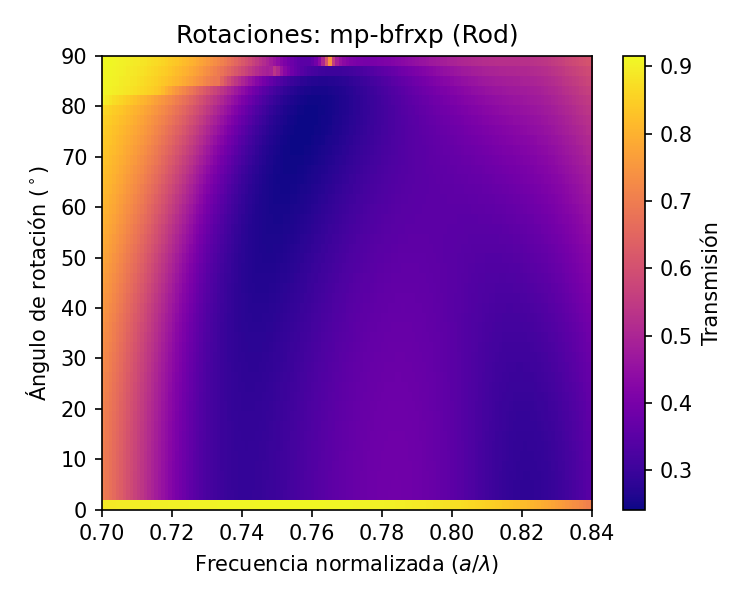
\includegraphics[width=0.48\textwidth]{figures/mp-bfrxp_rod_rangle.png}
\caption{Mapas de transmisión por rotación (twist) para mp-bfrxp. Izquierda: Lámina. Derecha: Cilindros.}
\end{figure}
\vspace{1em}
\hrule
\vspace{1em}
\subsection*{Material ID: mp-bfryn}
\textbf{Constante Dieléctrica ($\epsilon_{total}$):} 3.47 \\[0.5em]
\begin{table}[h!]
\centering
\begin{tabular}{lcc}
\toprule
\textbf{Métrica} & \textbf{Lámina (Plate)} & \textbf{Cilindros (Rod)} \\
\midrule
Bandgaps ($k_x$) & Ninguno & Ninguno \\
Resonancias ($k_x$) & 36 & 36 \\
\midrule
Bandgaps (Rotación) & Ninguno & Ninguno \\
Resonancias (Rotación) & 33 & 33 \\
\bottomrule
\end{tabular}
\end{table}
\begin{figure}[H]
\centering
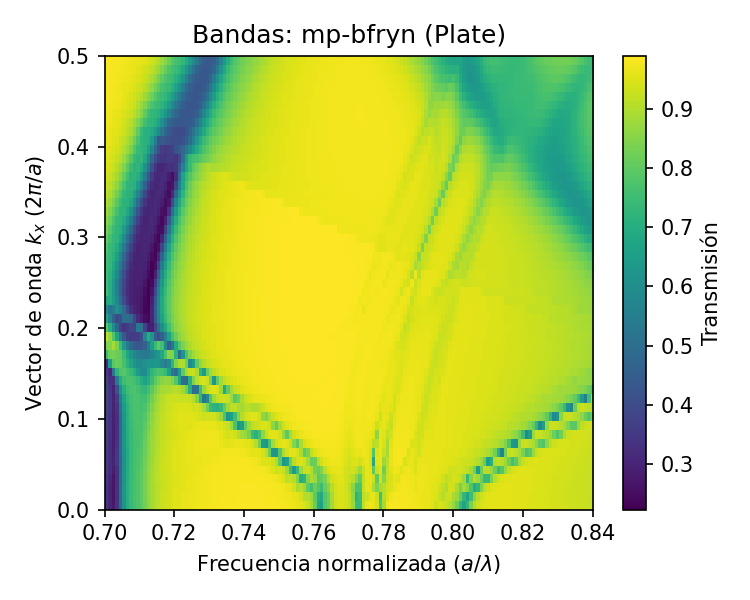
\includegraphics[width=0.48\textwidth]{figures/mp-bfryn_plate.png}
\hfill
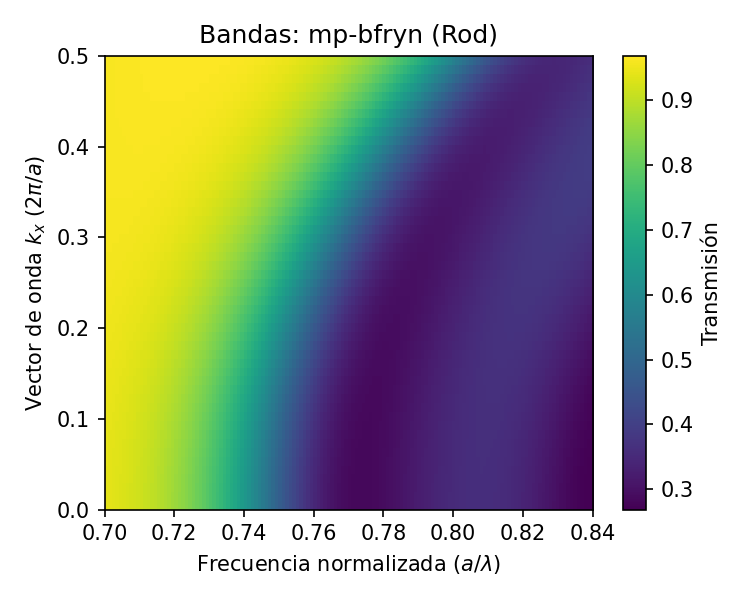
\includegraphics[width=0.48\textwidth]{figures/mp-bfryn_rod.png}
\caption{Estructuras de bandas fotónicas ($k_x$) para mp-bfryn. Izquierda: Lámina. Derecha: Cilindros.}
\end{figure}
\vspace{1em}
\begin{figure}[H]
\centering
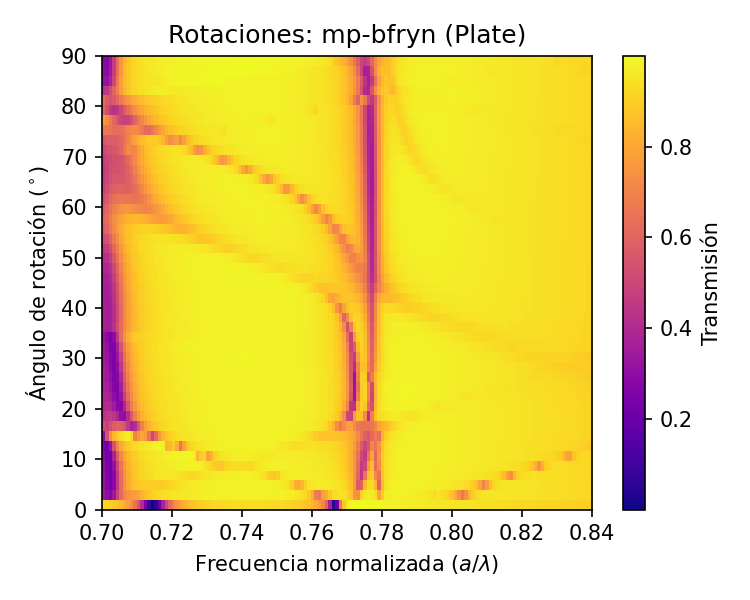
\includegraphics[width=0.48\textwidth]{figures/mp-bfryn_plate_rangle.png}
\hfill
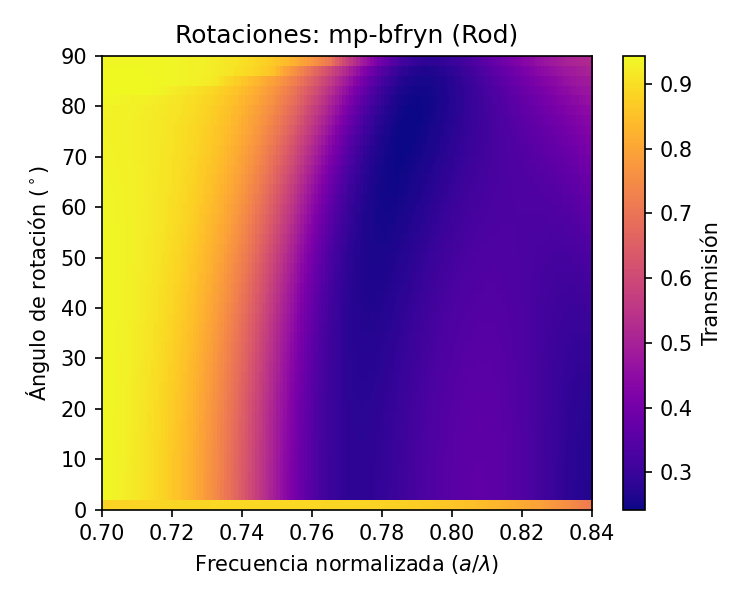
\includegraphics[width=0.48\textwidth]{figures/mp-bfryn_rod_rangle.png}
\caption{Mapas de transmisión por rotación (twist) para mp-bfryn. Izquierda: Lámina. Derecha: Cilindros.}
\end{figure}
\vspace{1em}
\hrule
\vspace{1em}
\subsection*{Material ID: mp-bfryw}
\textbf{Constante Dieléctrica ($\epsilon_{total}$):} 3.94 \\[0.5em]
\begin{table}[h!]
\centering
\begin{tabular}{lcc}
\toprule
\textbf{Métrica} & \textbf{Lámina (Plate)} & \textbf{Cilindros (Rod)} \\
\midrule
Bandgaps ($k_x$) & Ninguno & Ninguno \\
Resonancias ($k_x$) & 36 & 36 \\
\midrule
Bandgaps (Rotación) & Ninguno & Ninguno \\
Resonancias (Rotación) & 33 & 33 \\
\bottomrule
\end{tabular}
\end{table}
\begin{figure}[H]
\centering
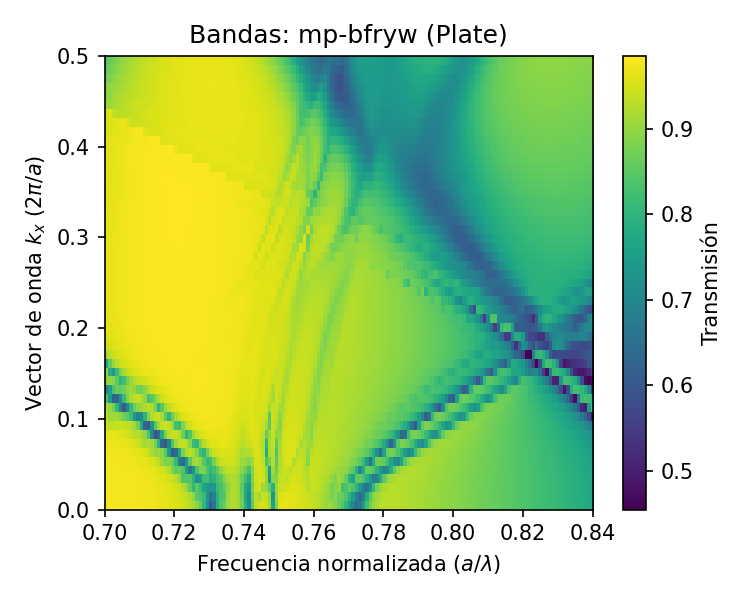
\includegraphics[width=0.48\textwidth]{figures/mp-bfryw_plate.png}
\hfill
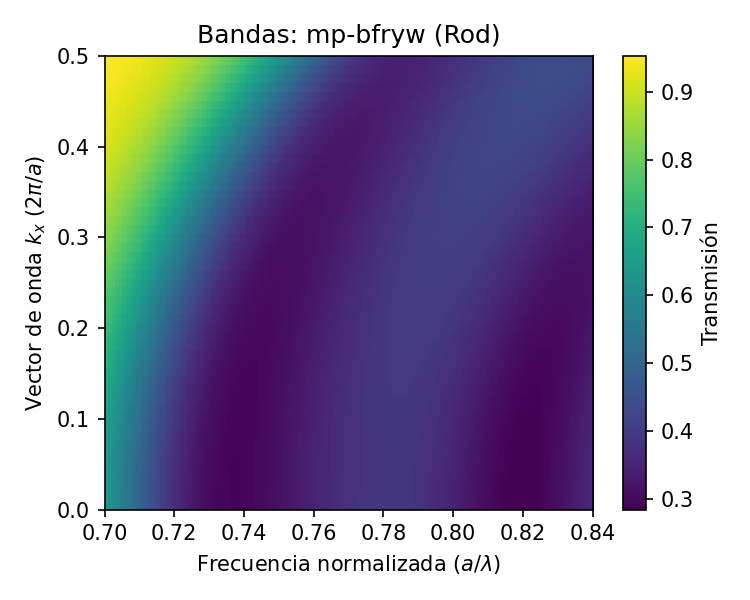
\includegraphics[width=0.48\textwidth]{figures/mp-bfryw_rod.png}
\caption{Estructuras de bandas fotónicas ($k_x$) para mp-bfryw. Izquierda: Lámina. Derecha: Cilindros.}
\end{figure}
\vspace{1em}
\begin{figure}[H]
\centering
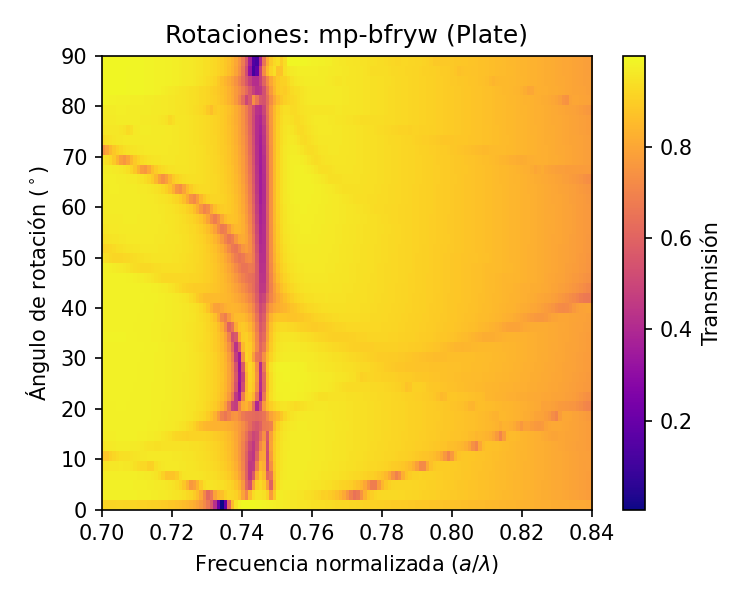
\includegraphics[width=0.48\textwidth]{figures/mp-bfryw_plate_rangle.png}
\hfill
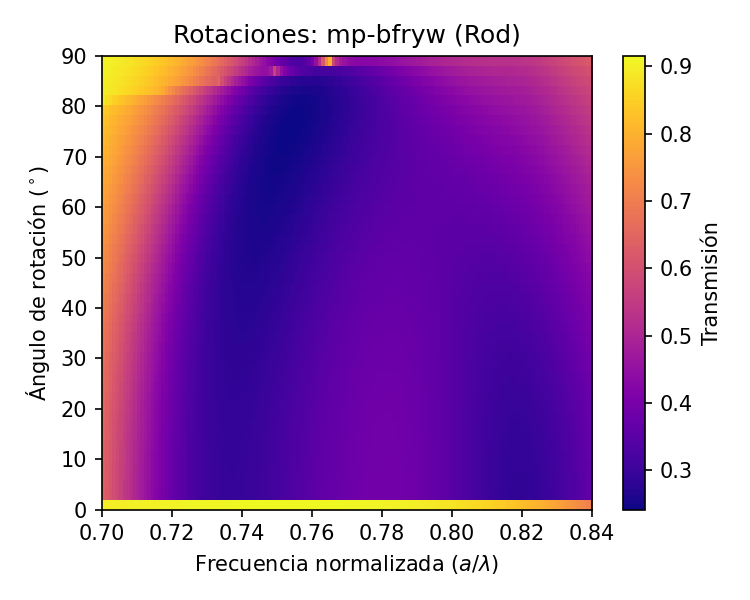
\includegraphics[width=0.48\textwidth]{figures/mp-bfryw_rod_rangle.png}
\caption{Mapas de transmisión por rotación (twist) para mp-bfryw. Izquierda: Lámina. Derecha: Cilindros.}
\end{figure}
\vspace{1em}
\hrule
\vspace{1em}
\subsection*{Material ID: mp-bfsdq}
\textbf{Constante Dieléctrica ($\epsilon_{total}$):} 4.37 \\[0.5em]
\begin{table}[h!]
\centering
\begin{tabular}{lcc}
\toprule
\textbf{Métrica} & \textbf{Lámina (Plate)} & \textbf{Cilindros (Rod)} \\
\midrule
Bandgaps ($k_x$) & Ninguno & Ninguno \\
Resonancias ($k_x$) & 36 & 36 \\
\midrule
Bandgaps (Rotación) & Ninguno & Ninguno \\
Resonancias (Rotación) & 33 & 33 \\
\bottomrule
\end{tabular}
\end{table}
\begin{figure}[H]
\centering
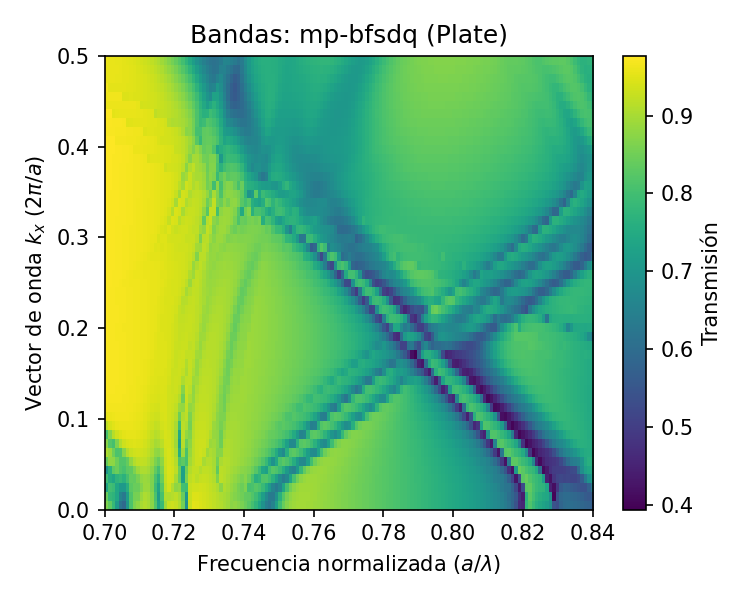
\includegraphics[width=0.48\textwidth]{figures/mp-bfsdq_plate.png}
\hfill
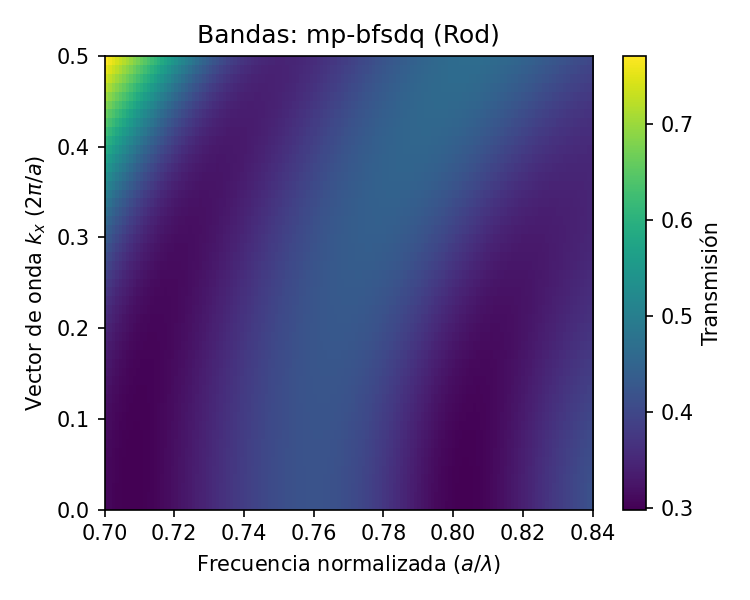
\includegraphics[width=0.48\textwidth]{figures/mp-bfsdq_rod.png}
\caption{Estructuras de bandas fotónicas ($k_x$) para mp-bfsdq. Izquierda: Lámina. Derecha: Cilindros.}
\end{figure}
\vspace{1em}
\begin{figure}[H]
\centering
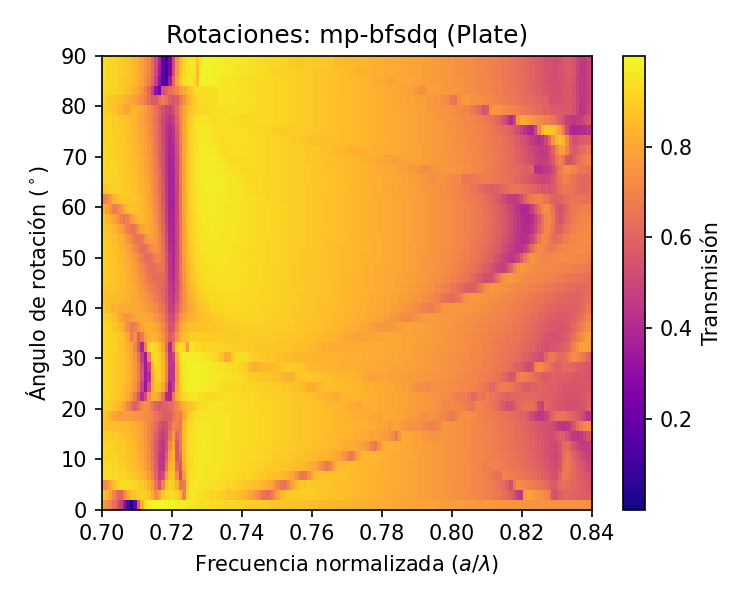
\includegraphics[width=0.48\textwidth]{figures/mp-bfsdq_plate_rangle.png}
\hfill
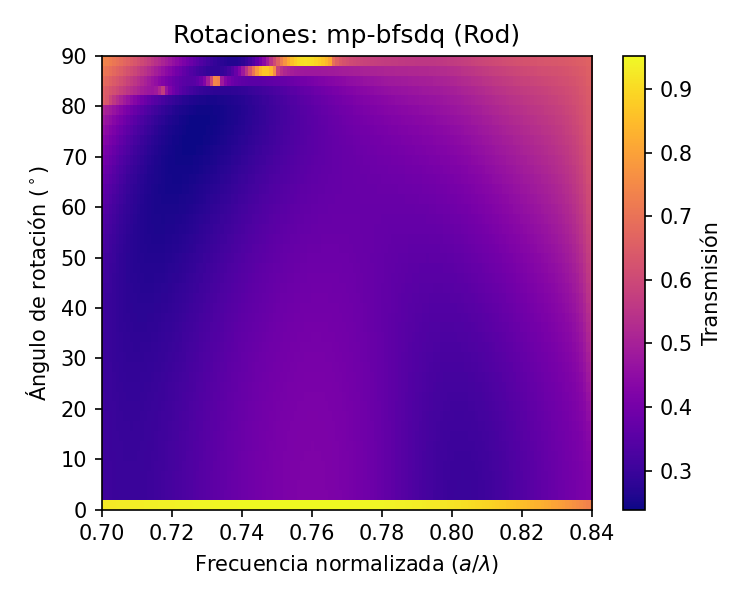
\includegraphics[width=0.48\textwidth]{figures/mp-bfsdq_rod_rangle.png}
\caption{Mapas de transmisión por rotación (twist) para mp-bfsdq. Izquierda: Lámina. Derecha: Cilindros.}
\end{figure}
\vspace{1em}
\hrule
\vspace{1em}
\subsection*{Material ID: mp-bfseg}
\textbf{Constante Dieléctrica ($\epsilon_{total}$):} 3.75 \\[0.5em]
\begin{table}[h!]
\centering
\begin{tabular}{lcc}
\toprule
\textbf{Métrica} & \textbf{Lámina (Plate)} & \textbf{Cilindros (Rod)} \\
\midrule
Bandgaps ($k_x$) & Ninguno & Ninguno \\
Resonancias ($k_x$) & 36 & 36 \\
\midrule
Bandgaps (Rotación) & Ninguno & Ninguno \\
Resonancias (Rotación) & 33 & 33 \\
\bottomrule
\end{tabular}
\end{table}
\begin{figure}[H]
\centering
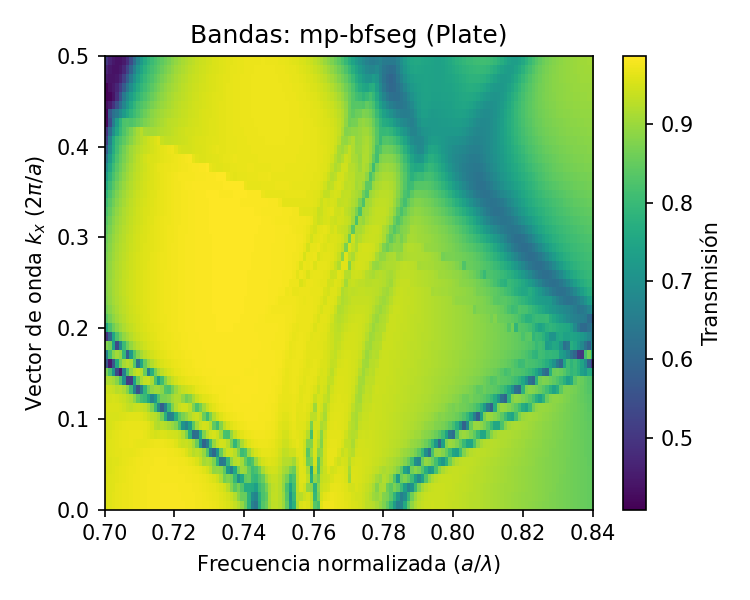
\includegraphics[width=0.48\textwidth]{figures/mp-bfseg_plate.png}
\hfill
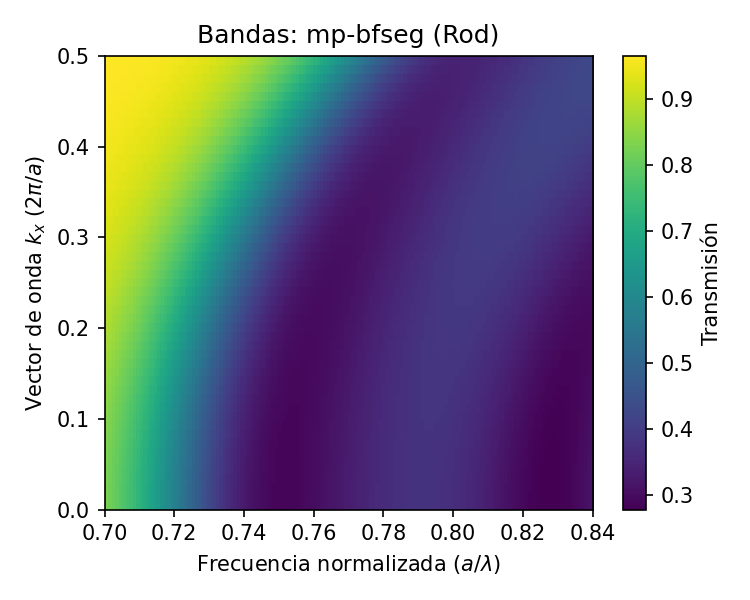
\includegraphics[width=0.48\textwidth]{figures/mp-bfseg_rod.png}
\caption{Estructuras de bandas fotónicas ($k_x$) para mp-bfseg. Izquierda: Lámina. Derecha: Cilindros.}
\end{figure}
\vspace{1em}
\begin{figure}[H]
\centering
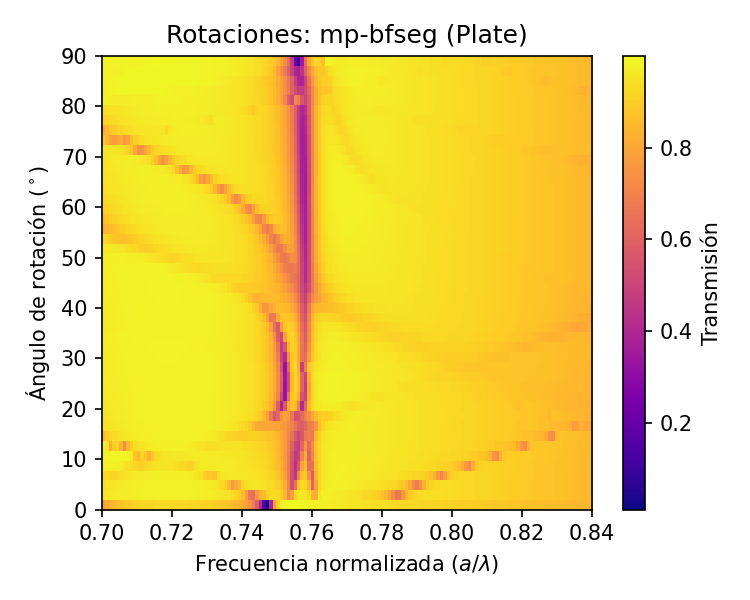
\includegraphics[width=0.48\textwidth]{figures/mp-bfseg_plate_rangle.png}
\hfill
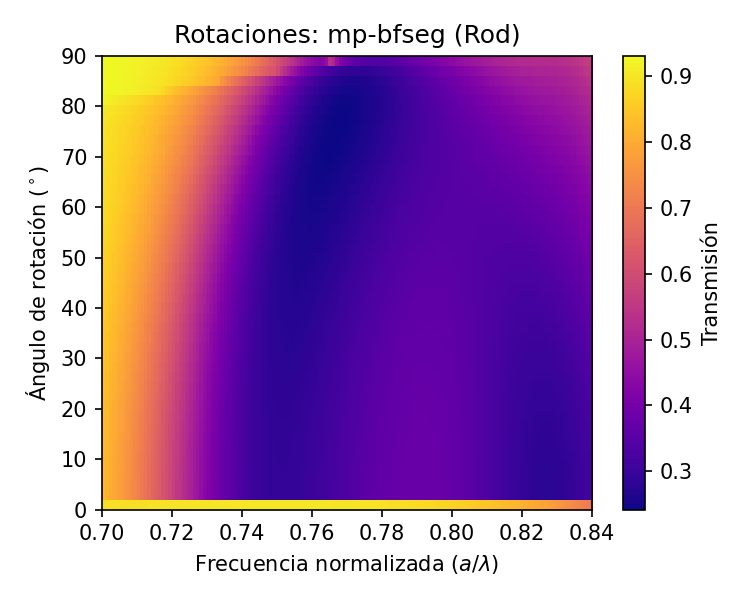
\includegraphics[width=0.48\textwidth]{figures/mp-bfseg_rod_rangle.png}
\caption{Mapas de transmisión por rotación (twist) para mp-bfseg. Izquierda: Lámina. Derecha: Cilindros.}
\end{figure}
\vspace{1em}
\hrule
\vspace{1em}
\subsection*{Material ID: mp-bfsim}
\textbf{Constante Dieléctrica ($\epsilon_{total}$):} 4.56 \\[0.5em]
\begin{table}[h!]
\centering
\begin{tabular}{lcc}
\toprule
\textbf{Métrica} & \textbf{Lámina (Plate)} & \textbf{Cilindros (Rod)} \\
\midrule
Bandgaps ($k_x$) & Ninguno & Ninguno \\
Resonancias ($k_x$) & 36 & 36 \\
\midrule
Bandgaps (Rotación) & Ninguno & Ninguno \\
Resonancias (Rotación) & 33 & 33 \\
\bottomrule
\end{tabular}
\end{table}
\begin{figure}[H]
\centering
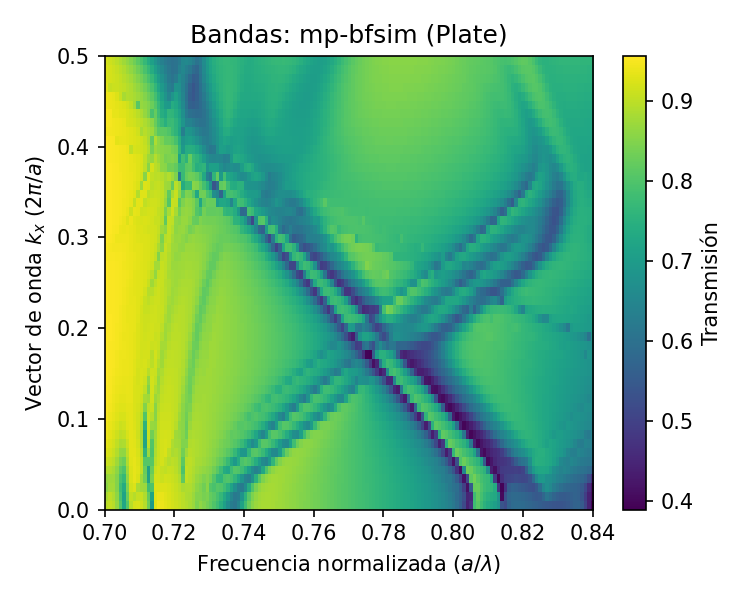
\includegraphics[width=0.48\textwidth]{figures/mp-bfsim_plate.png}
\hfill
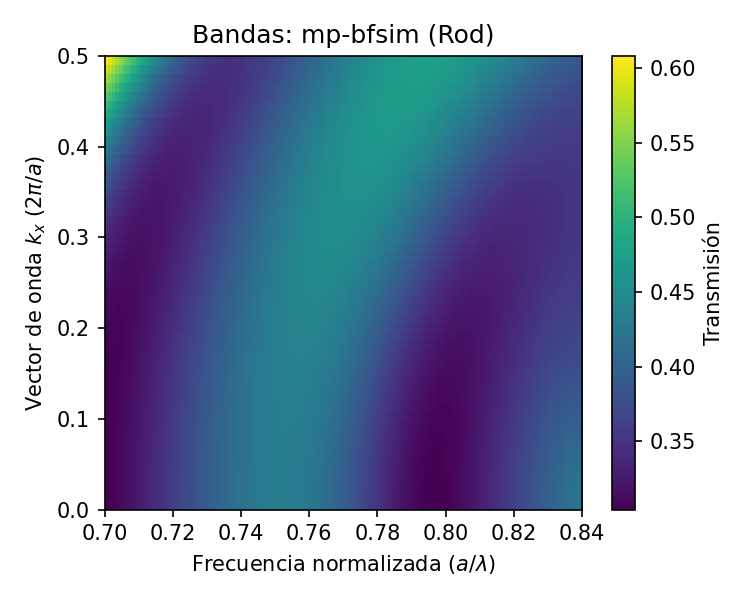
\includegraphics[width=0.48\textwidth]{figures/mp-bfsim_rod.png}
\caption{Estructuras de bandas fotónicas ($k_x$) para mp-bfsim. Izquierda: Lámina. Derecha: Cilindros.}
\end{figure}
\vspace{1em}
\begin{figure}[H]
\centering
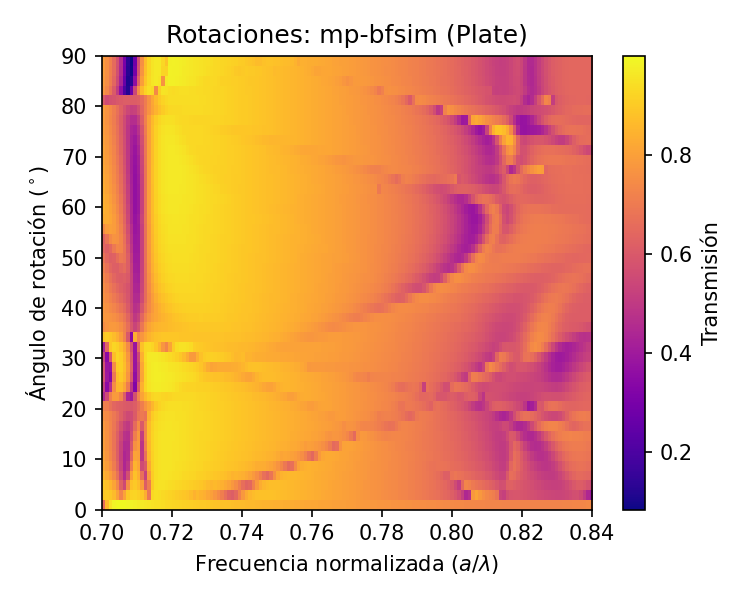
\includegraphics[width=0.48\textwidth]{figures/mp-bfsim_plate_rangle.png}
\hfill
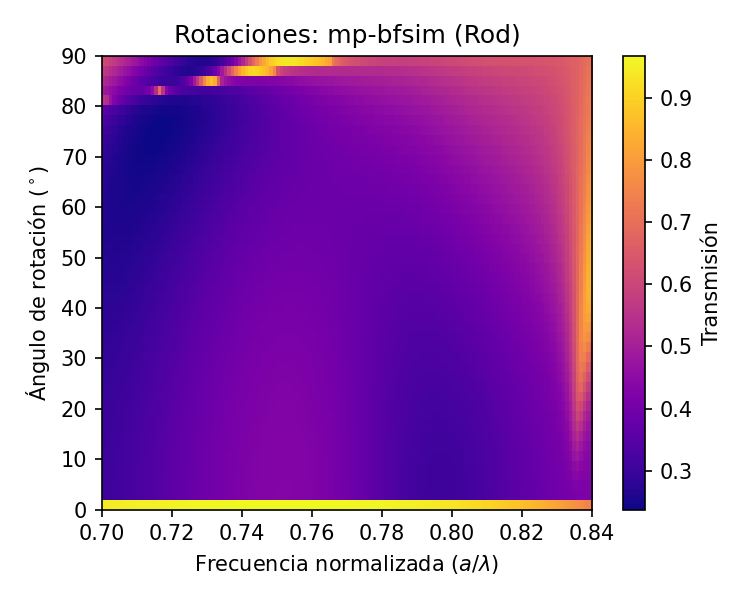
\includegraphics[width=0.48\textwidth]{figures/mp-bfsim_rod_rangle.png}
\caption{Mapas de transmisión por rotación (twist) para mp-bfsim. Izquierda: Lámina. Derecha: Cilindros.}
\end{figure}
\vspace{1em}
\hrule
\vspace{1em}
\subsection*{Material ID: mp-bfsqz}
\textbf{Constante Dieléctrica ($\epsilon_{total}$):} 4.52 \\[0.5em]
\begin{table}[h!]
\centering
\begin{tabular}{lcc}
\toprule
\textbf{Métrica} & \textbf{Lámina (Plate)} & \textbf{Cilindros (Rod)} \\
\midrule
Bandgaps ($k_x$) & Ninguno & Ninguno \\
Resonancias ($k_x$) & 36 & 36 \\
\midrule
Bandgaps (Rotación) & Ninguno & Ninguno \\
Resonancias (Rotación) & 33 & 33 \\
\bottomrule
\end{tabular}
\end{table}
\begin{figure}[H]
\centering
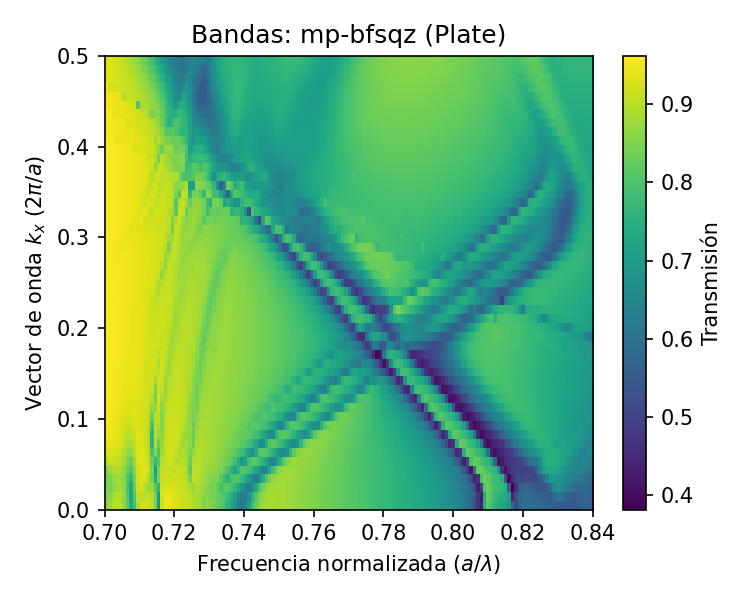
\includegraphics[width=0.48\textwidth]{figures/mp-bfsqz_plate.png}
\hfill
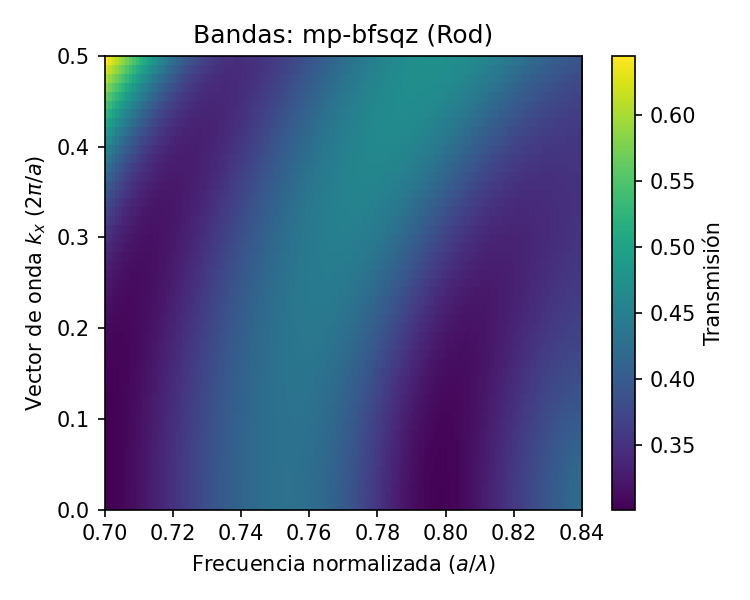
\includegraphics[width=0.48\textwidth]{figures/mp-bfsqz_rod.png}
\caption{Estructuras de bandas fotónicas ($k_x$) para mp-bfsqz. Izquierda: Lámina. Derecha: Cilindros.}
\end{figure}
\vspace{1em}
\begin{figure}[H]
\centering
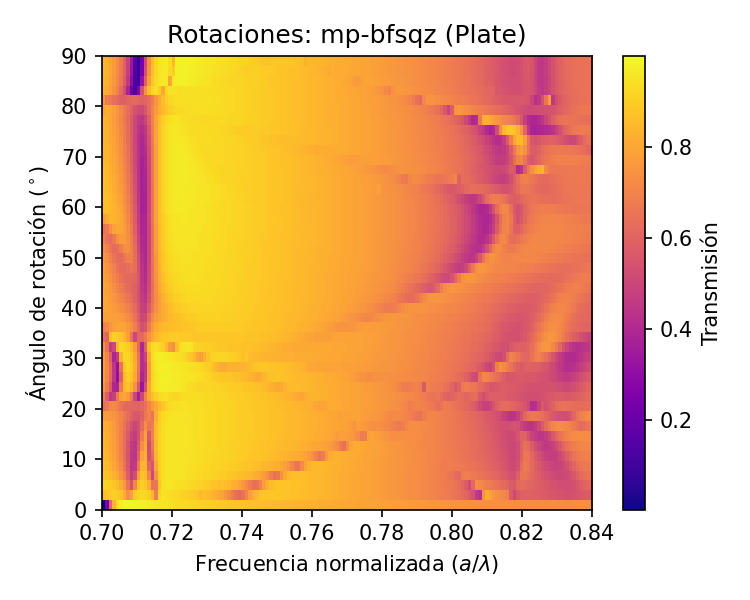
\includegraphics[width=0.48\textwidth]{figures/mp-bfsqz_plate_rangle.png}
\hfill
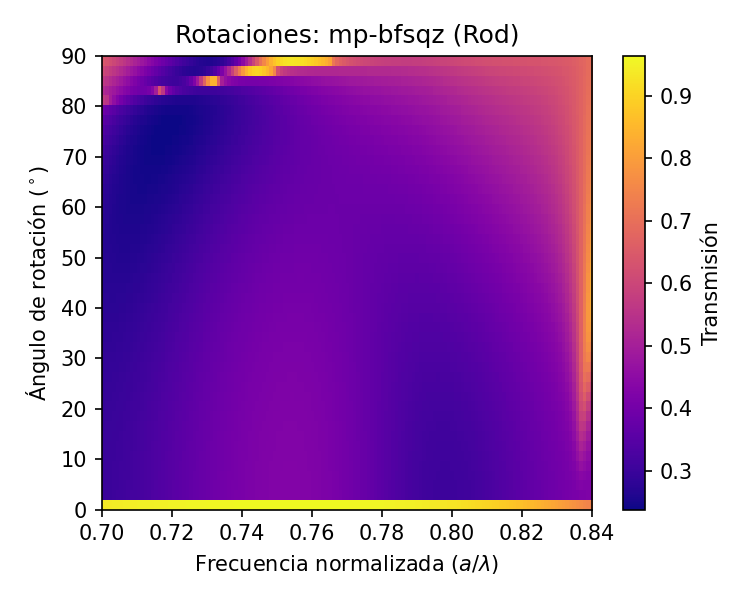
\includegraphics[width=0.48\textwidth]{figures/mp-bfsqz_rod_rangle.png}
\caption{Mapas de transmisión por rotación (twist) para mp-bfsqz. Izquierda: Lámina. Derecha: Cilindros.}
\end{figure}
\vspace{1em}
\hrule
\vspace{1em}
\subsection*{Material ID: mp-bfsyf}
\textbf{Constante Dieléctrica ($\epsilon_{total}$):} 5.35 \\[0.5em]
\begin{table}[h!]
\centering
\begin{tabular}{lcc}
\toprule
\textbf{Métrica} & \textbf{Lámina (Plate)} & \textbf{Cilindros (Rod)} \\
\midrule
Bandgaps ($k_x$) & Ninguno & Ninguno \\
Resonancias ($k_x$) & 36 & 36 \\
\midrule
Bandgaps (Rotación) & Ninguno & Ninguno \\
Resonancias (Rotación) & 33 & 33 \\
\bottomrule
\end{tabular}
\end{table}
\begin{figure}[H]
\centering
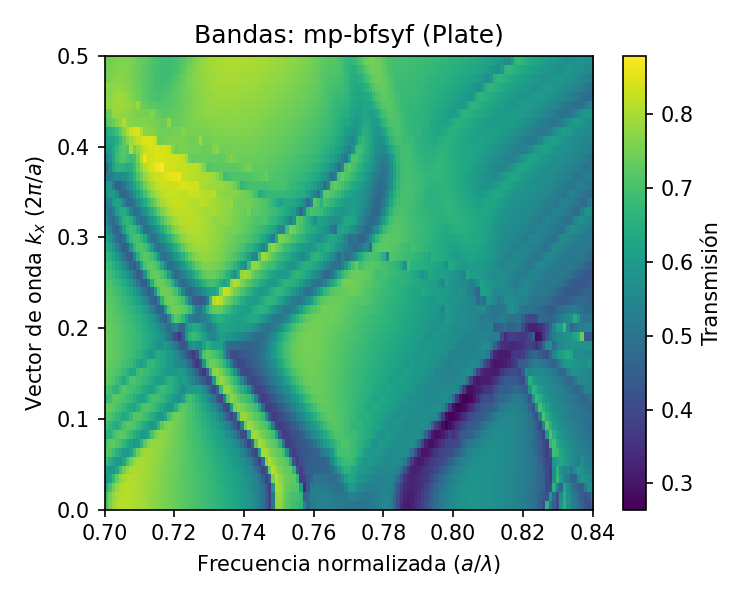
\includegraphics[width=0.48\textwidth]{figures/mp-bfsyf_plate.png}
\hfill
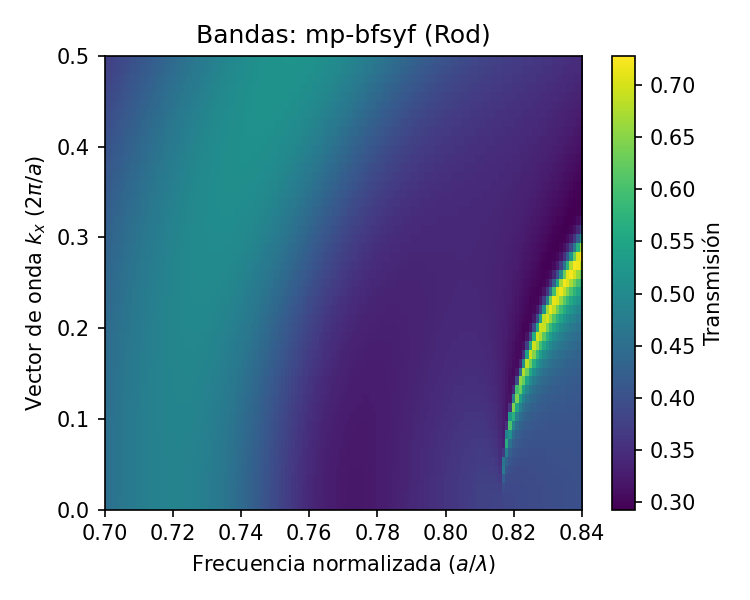
\includegraphics[width=0.48\textwidth]{figures/mp-bfsyf_rod.png}
\caption{Estructuras de bandas fotónicas ($k_x$) para mp-bfsyf. Izquierda: Lámina. Derecha: Cilindros.}
\end{figure}
\vspace{1em}
\begin{figure}[H]
\centering
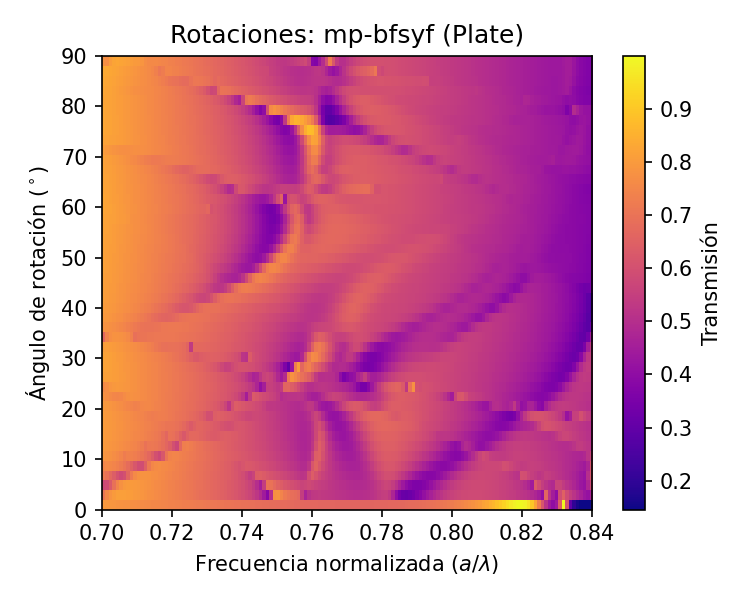
\includegraphics[width=0.48\textwidth]{figures/mp-bfsyf_plate_rangle.png}
\hfill
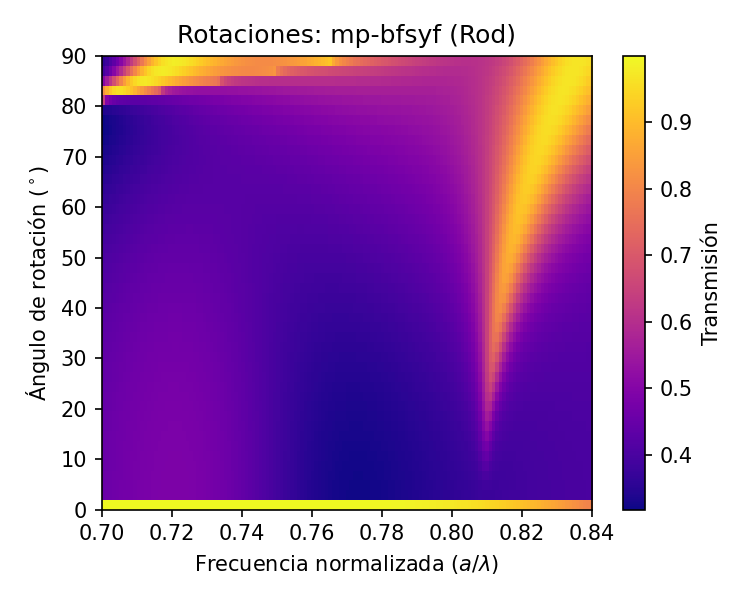
\includegraphics[width=0.48\textwidth]{figures/mp-bfsyf_rod_rangle.png}
\caption{Mapas de transmisión por rotación (twist) para mp-bfsyf. Izquierda: Lámina. Derecha: Cilindros.}
\end{figure}
\vspace{1em}
\hrule
\vspace{1em}
\subsection*{Material ID: mp-bftax}
\textbf{Constante Dieléctrica ($\epsilon_{total}$):} 5.08 \\[0.5em]
\begin{table}[h!]
\centering
\begin{tabular}{lcc}
\toprule
\textbf{Métrica} & \textbf{Lámina (Plate)} & \textbf{Cilindros (Rod)} \\
\midrule
Bandgaps ($k_x$) & Ninguno & Ninguno \\
Resonancias ($k_x$) & 36 & 36 \\
\midrule
Bandgaps (Rotación) & Ninguno & Ninguno \\
Resonancias (Rotación) & 33 & 33 \\
\bottomrule
\end{tabular}
\end{table}
\begin{figure}[H]
\centering
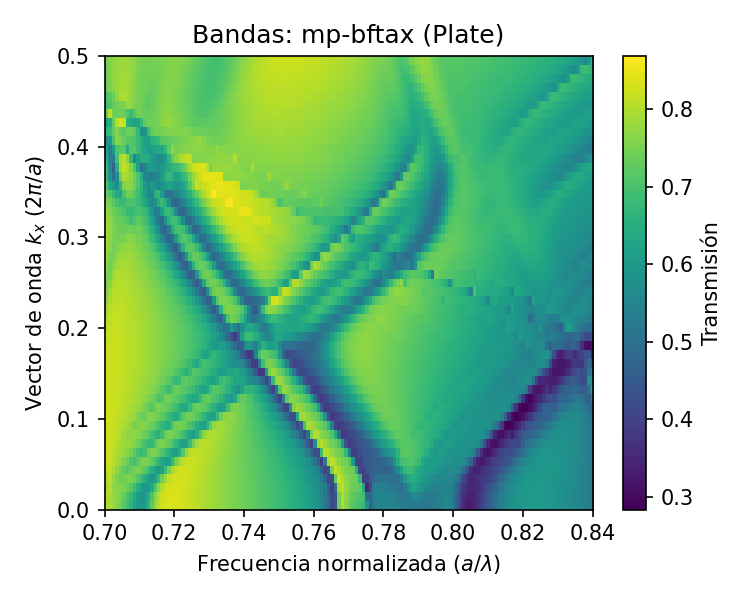
\includegraphics[width=0.48\textwidth]{figures/mp-bftax_plate.png}
\hfill
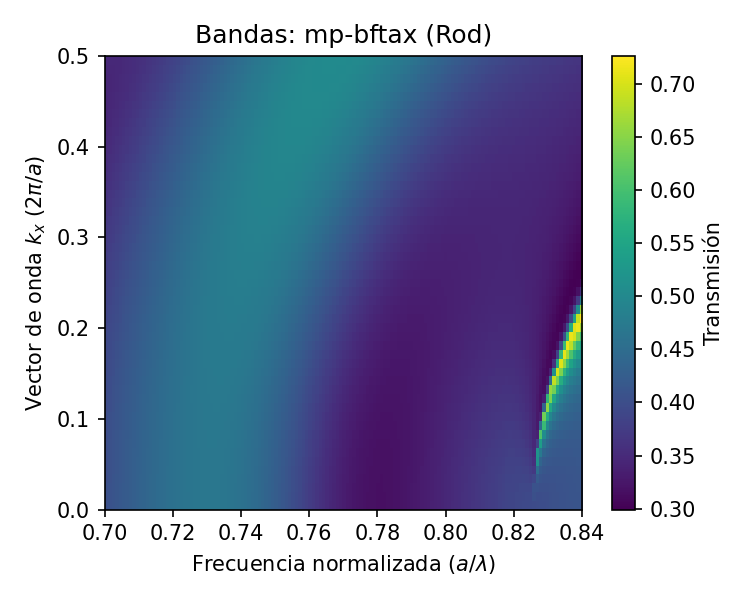
\includegraphics[width=0.48\textwidth]{figures/mp-bftax_rod.png}
\caption{Estructuras de bandas fotónicas ($k_x$) para mp-bftax. Izquierda: Lámina. Derecha: Cilindros.}
\end{figure}
\vspace{1em}
\begin{figure}[H]
\centering
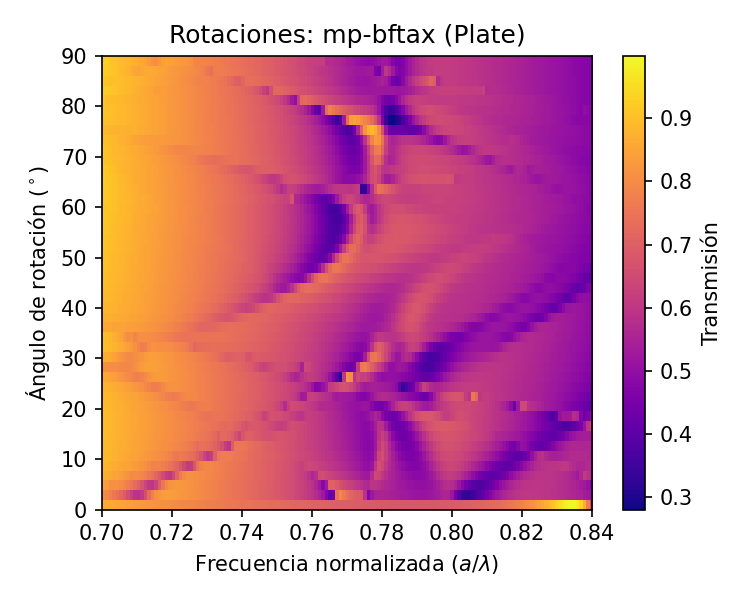
\includegraphics[width=0.48\textwidth]{figures/mp-bftax_plate_rangle.png}
\hfill
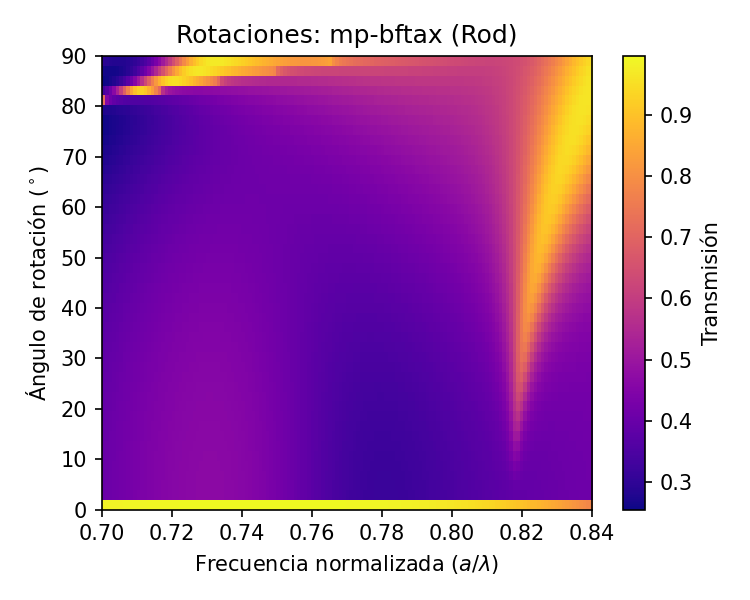
\includegraphics[width=0.48\textwidth]{figures/mp-bftax_rod_rangle.png}
\caption{Mapas de transmisión por rotación (twist) para mp-bftax. Izquierda: Lámina. Derecha: Cilindros.}
\end{figure}
\vspace{1em}
\hrule
\vspace{1em}
\subsection*{Material ID: mp-bftfh}
\textbf{Constante Dieléctrica ($\epsilon_{total}$):} 4.14 \\[0.5em]
\begin{table}[h!]
\centering
\begin{tabular}{lcc}
\toprule
\textbf{Métrica} & \textbf{Lámina (Plate)} & \textbf{Cilindros (Rod)} \\
\midrule
Bandgaps ($k_x$) & Ninguno & Ninguno \\
Resonancias ($k_x$) & 36 & 36 \\
\midrule
Bandgaps (Rotación) & Ninguno & Ninguno \\
Resonancias (Rotación) & 33 & 33 \\
\bottomrule
\end{tabular}
\end{table}
\begin{figure}[H]
\centering
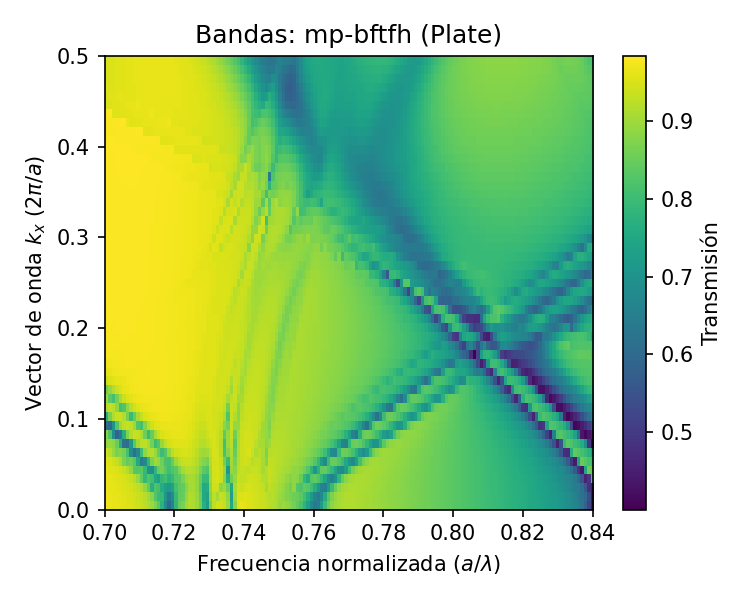
\includegraphics[width=0.48\textwidth]{figures/mp-bftfh_plate.png}
\hfill
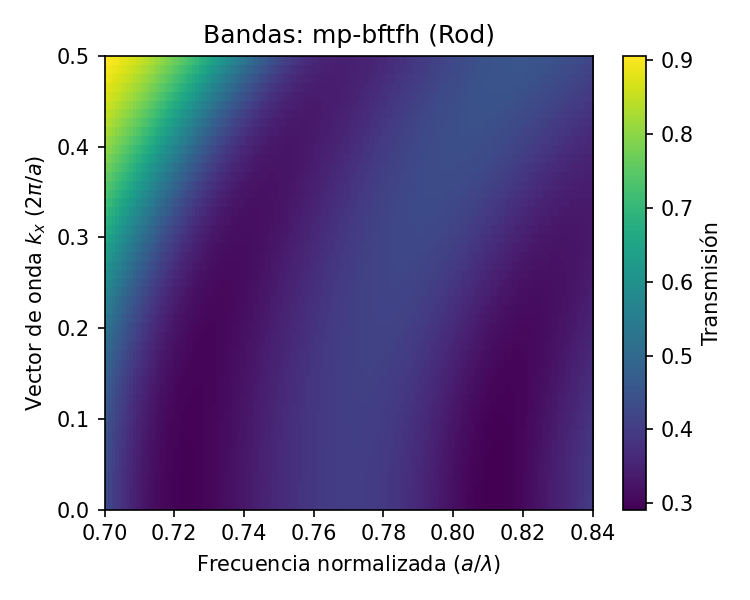
\includegraphics[width=0.48\textwidth]{figures/mp-bftfh_rod.png}
\caption{Estructuras de bandas fotónicas ($k_x$) para mp-bftfh. Izquierda: Lámina. Derecha: Cilindros.}
\end{figure}
\vspace{1em}
\begin{figure}[H]
\centering
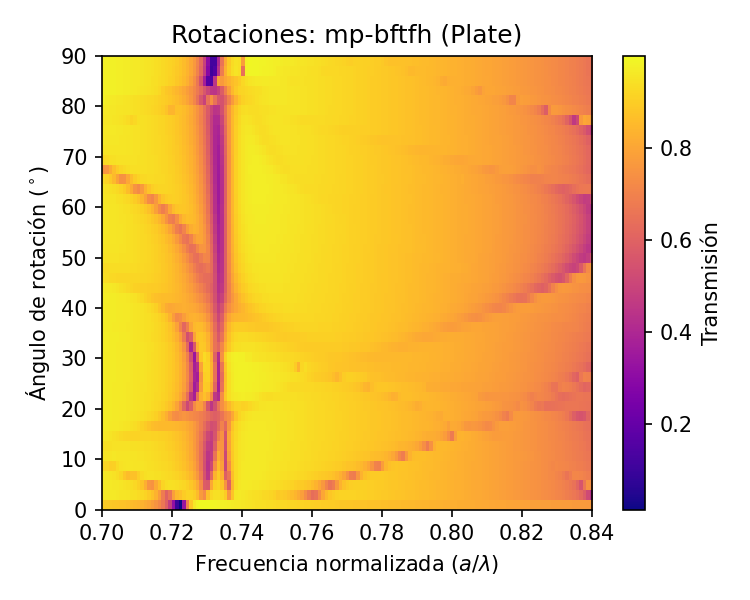
\includegraphics[width=0.48\textwidth]{figures/mp-bftfh_plate_rangle.png}
\hfill
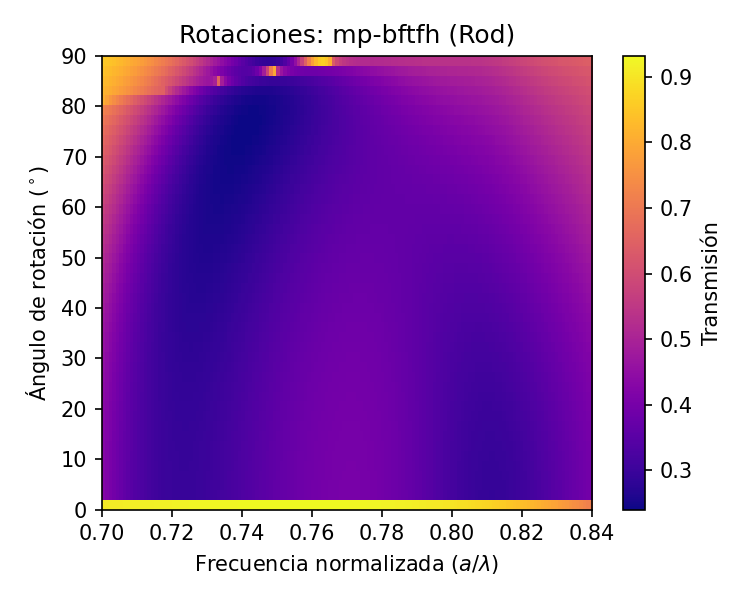
\includegraphics[width=0.48\textwidth]{figures/mp-bftfh_rod_rangle.png}
\caption{Mapas de transmisión por rotación (twist) para mp-bftfh. Izquierda: Lámina. Derecha: Cilindros.}
\end{figure}
\vspace{1em}
\hrule
\vspace{1em}
\subsection*{Material ID: mp-bftgz}
\textbf{Constante Dieléctrica ($\epsilon_{total}$):} 3.25 \\[0.5em]
\begin{table}[h!]
\centering
\begin{tabular}{lcc}
\toprule
\textbf{Métrica} & \textbf{Lámina (Plate)} & \textbf{Cilindros (Rod)} \\
\midrule
Bandgaps ($k_x$) & Ninguno & Ninguno \\
Resonancias ($k_x$) & 36 & 36 \\
\midrule
Bandgaps (Rotación) & Ninguno & Ninguno \\
Resonancias (Rotación) & 33 & 33 \\
\bottomrule
\end{tabular}
\end{table}
\begin{figure}[H]
\centering
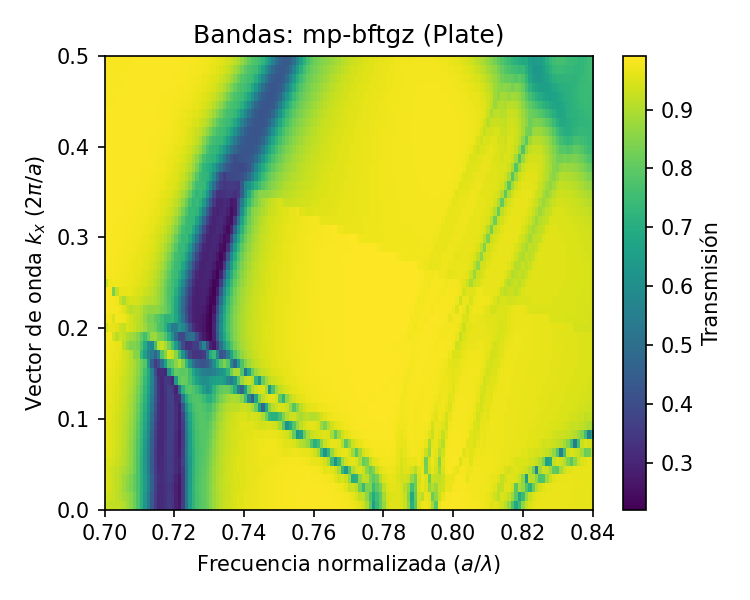
\includegraphics[width=0.48\textwidth]{figures/mp-bftgz_plate.png}
\hfill
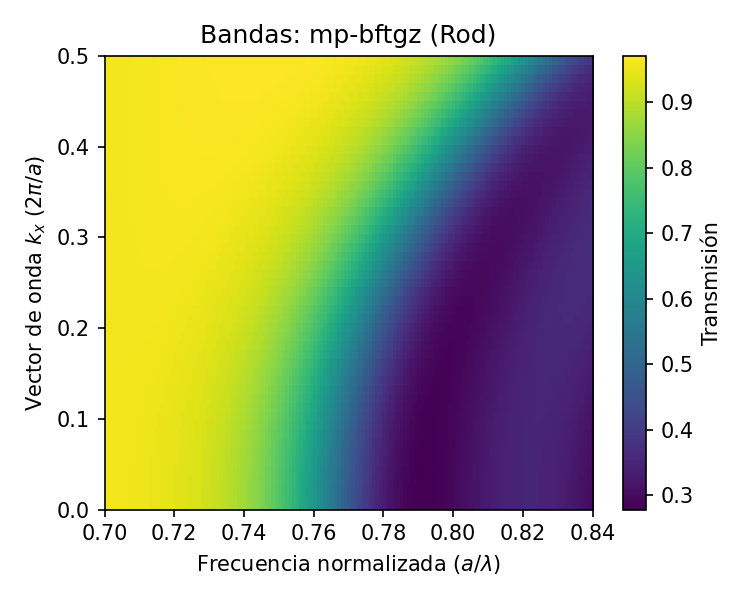
\includegraphics[width=0.48\textwidth]{figures/mp-bftgz_rod.png}
\caption{Estructuras de bandas fotónicas ($k_x$) para mp-bftgz. Izquierda: Lámina. Derecha: Cilindros.}
\end{figure}
\vspace{1em}
\begin{figure}[H]
\centering
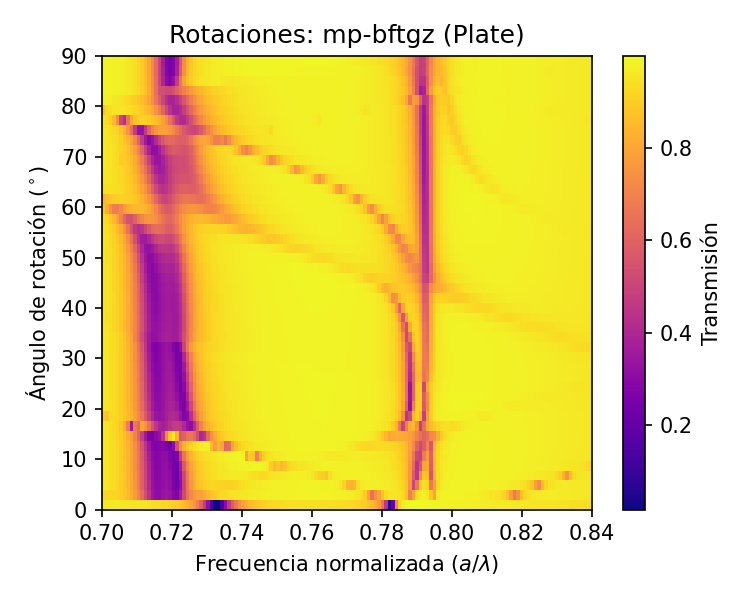
\includegraphics[width=0.48\textwidth]{figures/mp-bftgz_plate_rangle.png}
\hfill
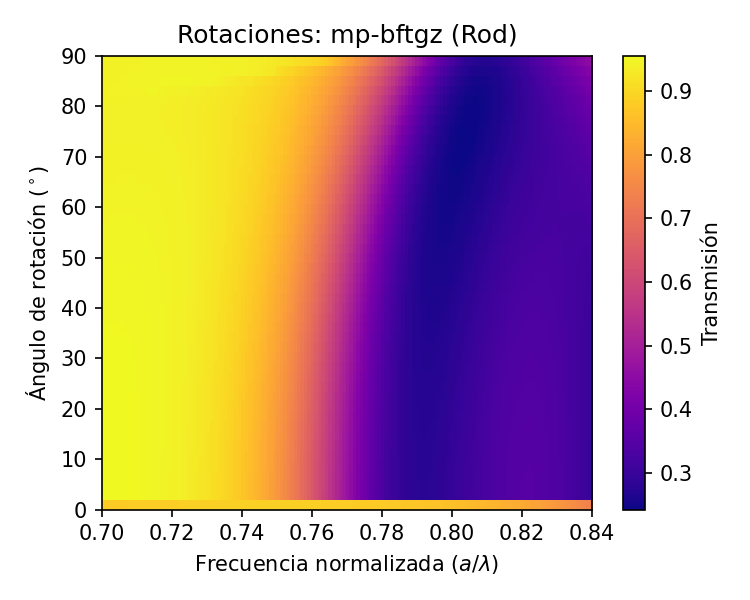
\includegraphics[width=0.48\textwidth]{figures/mp-bftgz_rod_rangle.png}
\caption{Mapas de transmisión por rotación (twist) para mp-bftgz. Izquierda: Lámina. Derecha: Cilindros.}
\end{figure}
\vspace{1em}
\hrule
\vspace{1em}
\subsection*{Material ID: mp-bftiw}
\textbf{Constante Dieléctrica ($\epsilon_{total}$):} 4.09 \\[0.5em]
\begin{table}[h!]
\centering
\begin{tabular}{lcc}
\toprule
\textbf{Métrica} & \textbf{Lámina (Plate)} & \textbf{Cilindros (Rod)} \\
\midrule
Bandgaps ($k_x$) & Ninguno & Ninguno \\
Resonancias ($k_x$) & 36 & 36 \\
\midrule
Bandgaps (Rotación) & Ninguno & Ninguno \\
Resonancias (Rotación) & 33 & 33 \\
\bottomrule
\end{tabular}
\end{table}
\begin{figure}[H]
\centering
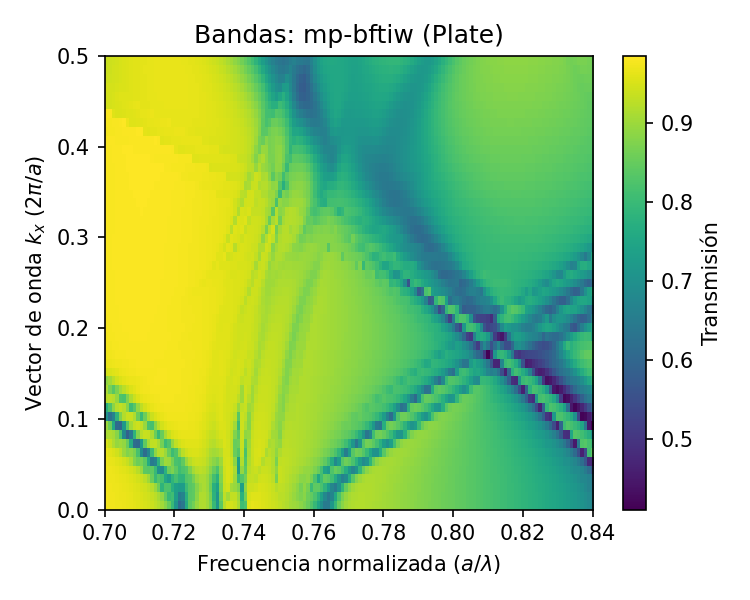
\includegraphics[width=0.48\textwidth]{figures/mp-bftiw_plate.png}
\hfill
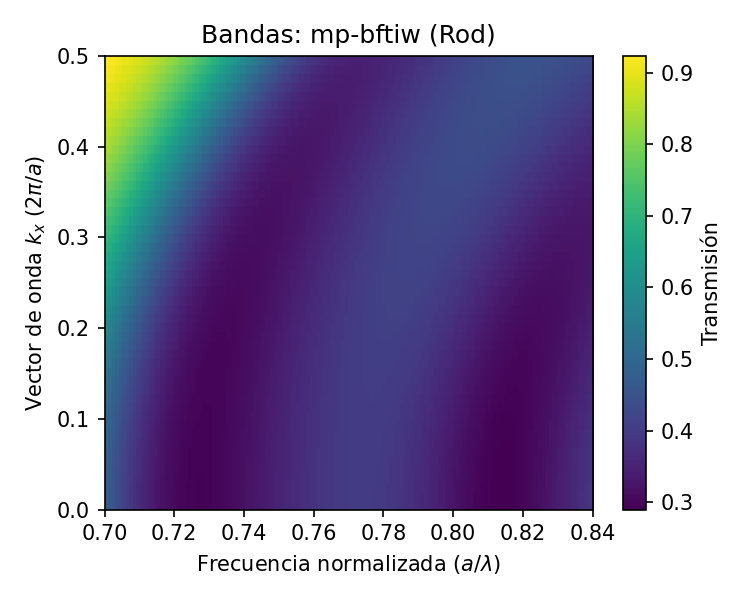
\includegraphics[width=0.48\textwidth]{figures/mp-bftiw_rod.png}
\caption{Estructuras de bandas fotónicas ($k_x$) para mp-bftiw. Izquierda: Lámina. Derecha: Cilindros.}
\end{figure}
\vspace{1em}
\begin{figure}[H]
\centering
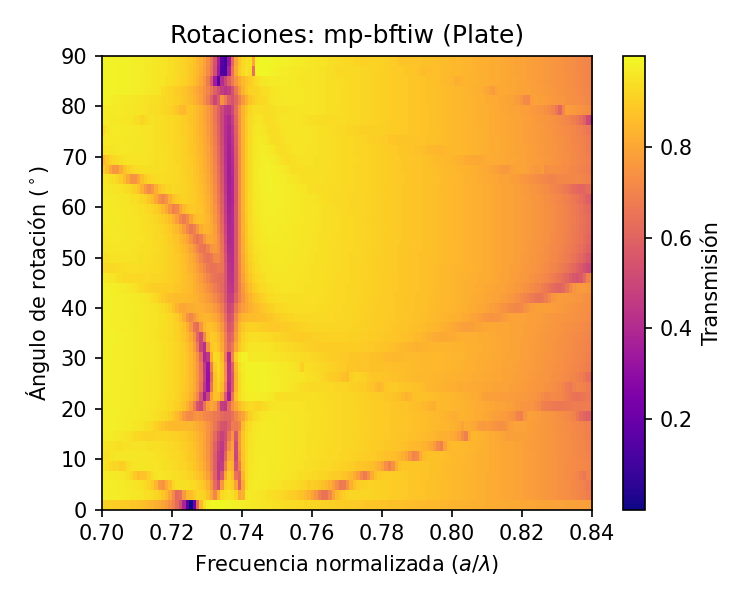
\includegraphics[width=0.48\textwidth]{figures/mp-bftiw_plate_rangle.png}
\hfill
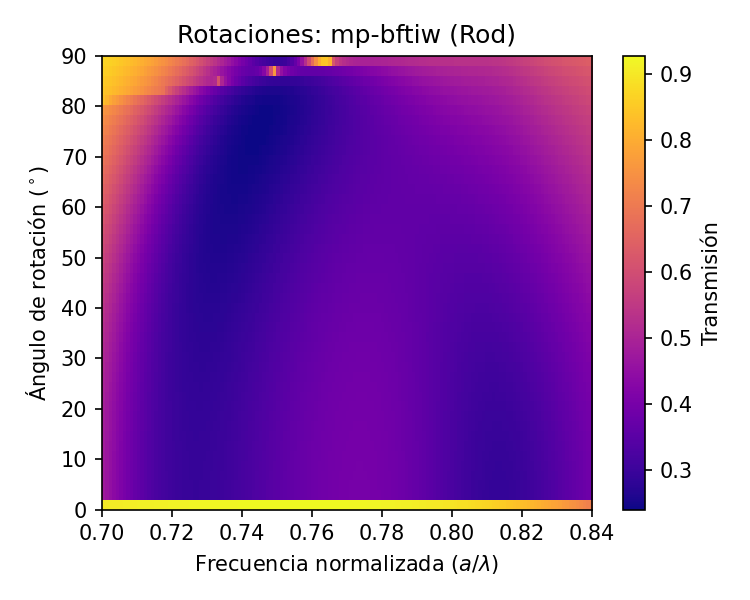
\includegraphics[width=0.48\textwidth]{figures/mp-bftiw_rod_rangle.png}
\caption{Mapas de transmisión por rotación (twist) para mp-bftiw. Izquierda: Lámina. Derecha: Cilindros.}
\end{figure}
\vspace{1em}
\hrule
\vspace{1em}
\subsection*{Material ID: mp-bfttg}
\textbf{Constante Dieléctrica ($\epsilon_{total}$):} 4.24 \\[0.5em]
\begin{table}[h!]
\centering
\begin{tabular}{lcc}
\toprule
\textbf{Métrica} & \textbf{Lámina (Plate)} & \textbf{Cilindros (Rod)} \\
\midrule
Bandgaps ($k_x$) & Ninguno & Ninguno \\
Resonancias ($k_x$) & 36 & 36 \\
\midrule
Bandgaps (Rotación) & Ninguno & Ninguno \\
Resonancias (Rotación) & 33 & 33 \\
\bottomrule
\end{tabular}
\end{table}
\begin{figure}[H]
\centering
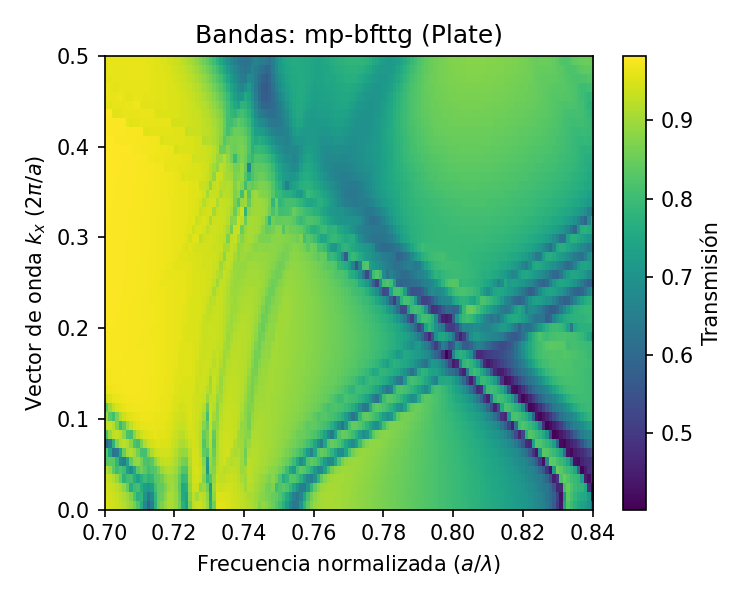
\includegraphics[width=0.48\textwidth]{figures/mp-bfttg_plate.png}
\hfill
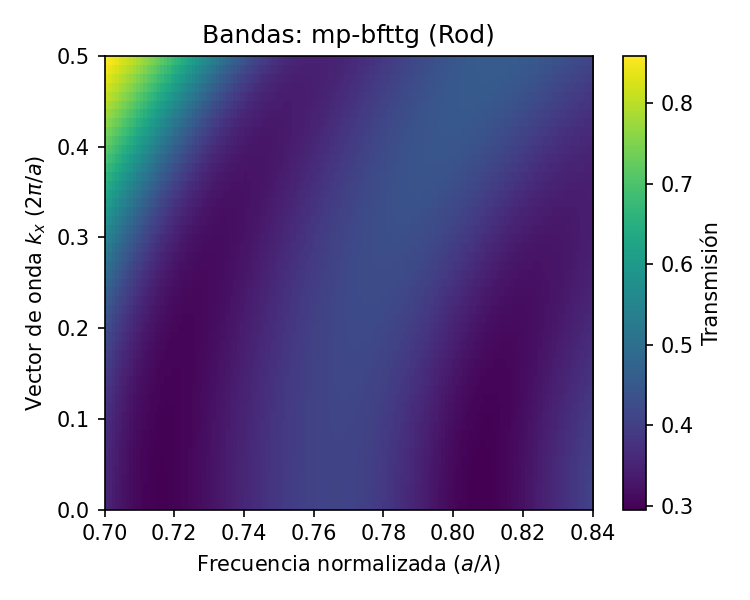
\includegraphics[width=0.48\textwidth]{figures/mp-bfttg_rod.png}
\caption{Estructuras de bandas fotónicas ($k_x$) para mp-bfttg. Izquierda: Lámina. Derecha: Cilindros.}
\end{figure}
\vspace{1em}
\begin{figure}[H]
\centering
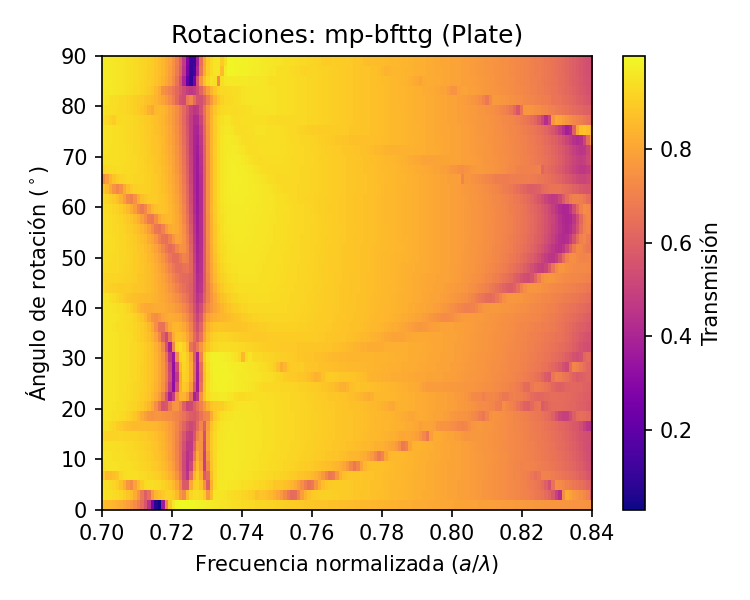
\includegraphics[width=0.48\textwidth]{figures/mp-bfttg_plate_rangle.png}
\hfill
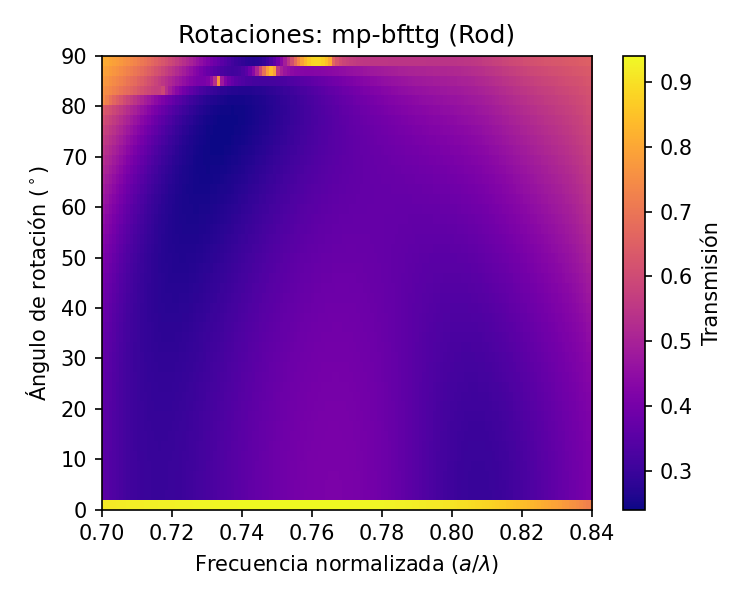
\includegraphics[width=0.48\textwidth]{figures/mp-bfttg_rod_rangle.png}
\caption{Mapas de transmisión por rotación (twist) para mp-bfttg. Izquierda: Lámina. Derecha: Cilindros.}
\end{figure}
\vspace{1em}
\hrule
\vspace{1em}
\subsection*{Material ID: mp-bfutv}
\textbf{Constante Dieléctrica ($\epsilon_{total}$):} 4.15 \\[0.5em]
\begin{table}[h!]
\centering
\begin{tabular}{lcc}
\toprule
\textbf{Métrica} & \textbf{Lámina (Plate)} & \textbf{Cilindros (Rod)} \\
\midrule
Bandgaps ($k_x$) & Ninguno & Ninguno \\
Resonancias ($k_x$) & 36 & 36 \\
\midrule
Bandgaps (Rotación) & Ninguno & Ninguno \\
Resonancias (Rotación) & 33 & 33 \\
\bottomrule
\end{tabular}
\end{table}
\begin{figure}[H]
\centering
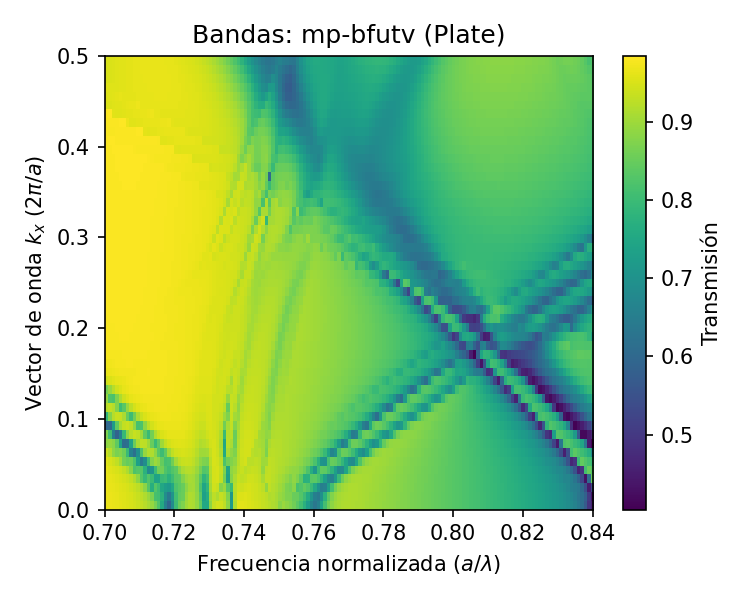
\includegraphics[width=0.48\textwidth]{figures/mp-bfutv_plate.png}
\hfill
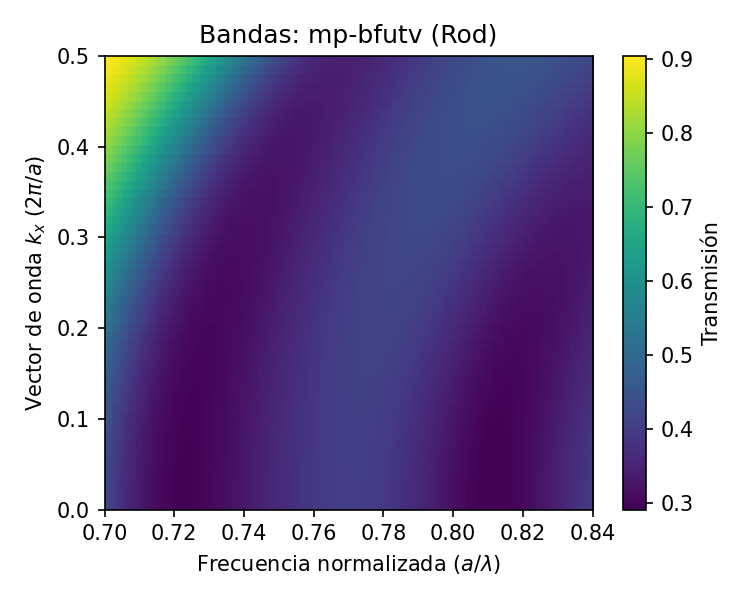
\includegraphics[width=0.48\textwidth]{figures/mp-bfutv_rod.png}
\caption{Estructuras de bandas fotónicas ($k_x$) para mp-bfutv. Izquierda: Lámina. Derecha: Cilindros.}
\end{figure}
\vspace{1em}
\begin{figure}[H]
\centering
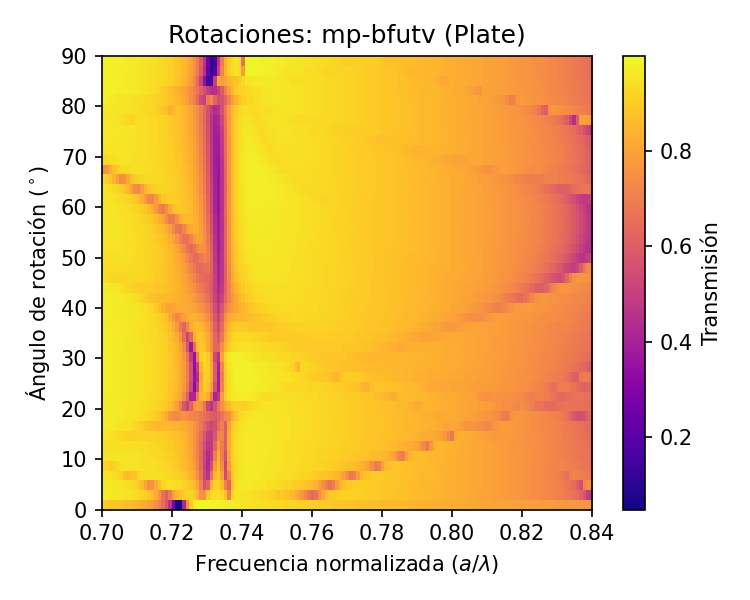
\includegraphics[width=0.48\textwidth]{figures/mp-bfutv_plate_rangle.png}
\hfill
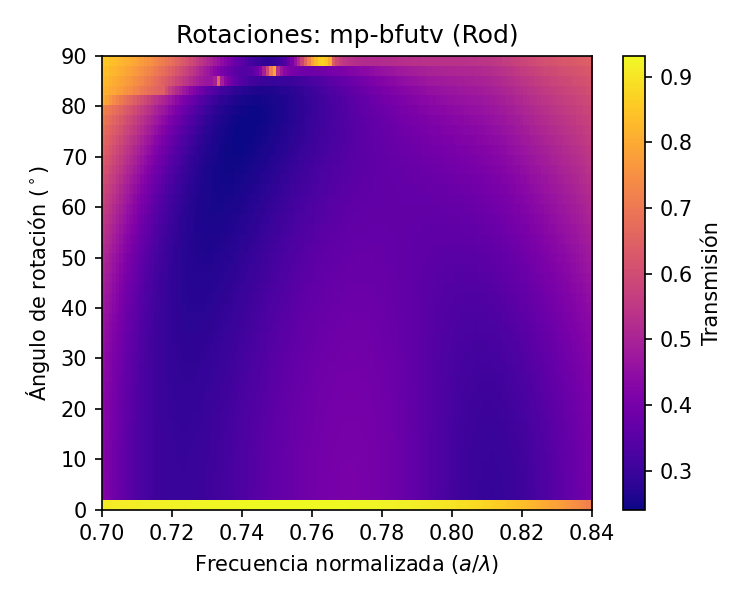
\includegraphics[width=0.48\textwidth]{figures/mp-bfutv_rod_rangle.png}
\caption{Mapas de transmisión por rotación (twist) para mp-bfutv. Izquierda: Lámina. Derecha: Cilindros.}
\end{figure}
\vspace{1em}
\hrule
\vspace{1em}
\subsection*{Material ID: mp-bfvbn}
\textbf{Constante Dieléctrica ($\epsilon_{total}$):} 3.84 \\[0.5em]
\begin{table}[h!]
\centering
\begin{tabular}{lcc}
\toprule
\textbf{Métrica} & \textbf{Lámina (Plate)} & \textbf{Cilindros (Rod)} \\
\midrule
Bandgaps ($k_x$) & Ninguno & Ninguno \\
Resonancias ($k_x$) & 36 & 36 \\
\midrule
Bandgaps (Rotación) & Ninguno & Ninguno \\
Resonancias (Rotación) & 33 & 33 \\
\bottomrule
\end{tabular}
\end{table}
\begin{figure}[H]
\centering
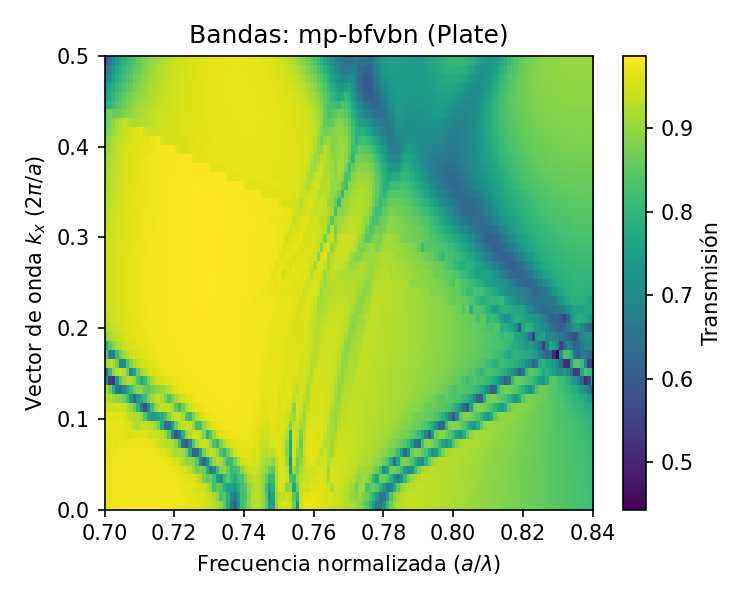
\includegraphics[width=0.48\textwidth]{figures/mp-bfvbn_plate.png}
\hfill
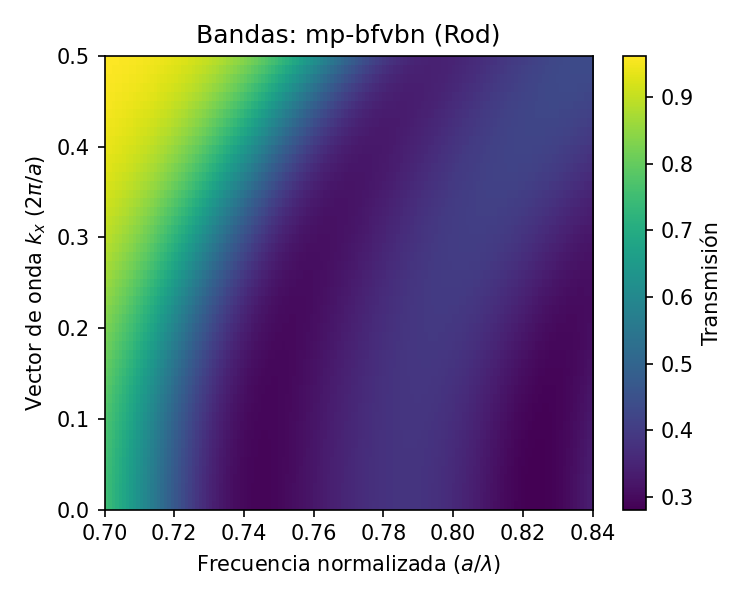
\includegraphics[width=0.48\textwidth]{figures/mp-bfvbn_rod.png}
\caption{Estructuras de bandas fotónicas ($k_x$) para mp-bfvbn. Izquierda: Lámina. Derecha: Cilindros.}
\end{figure}
\vspace{1em}
\begin{figure}[H]
\centering
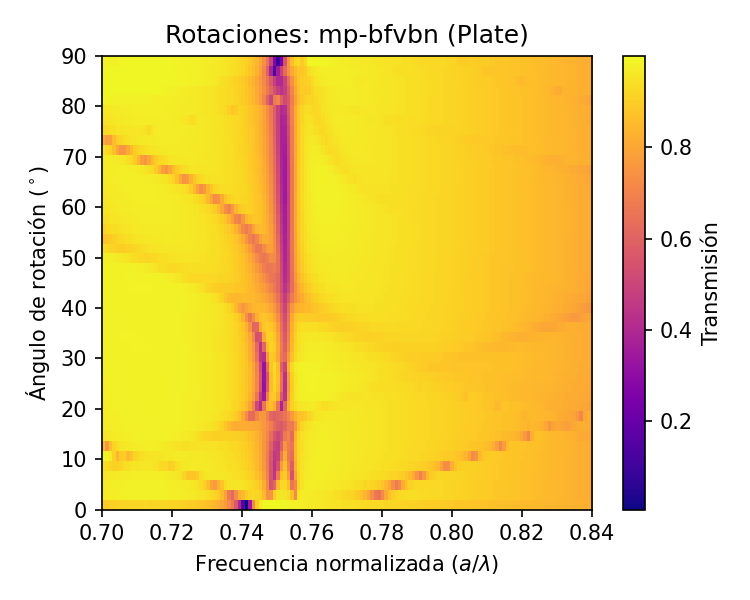
\includegraphics[width=0.48\textwidth]{figures/mp-bfvbn_plate_rangle.png}
\hfill
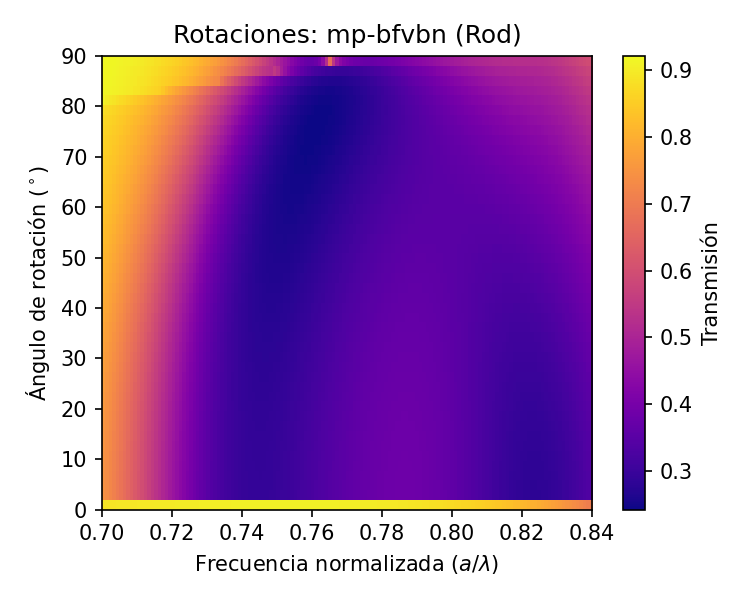
\includegraphics[width=0.48\textwidth]{figures/mp-bfvbn_rod_rangle.png}
\caption{Mapas de transmisión por rotación (twist) para mp-bfvbn. Izquierda: Lámina. Derecha: Cilindros.}
\end{figure}
\vspace{1em}
\hrule
\vspace{1em}
\subsection*{Material ID: mp-bfvkb}
\textbf{Constante Dieléctrica ($\epsilon_{total}$):} 3.66 \\[0.5em]
\begin{table}[h!]
\centering
\begin{tabular}{lcc}
\toprule
\textbf{Métrica} & \textbf{Lámina (Plate)} & \textbf{Cilindros (Rod)} \\
\midrule
Bandgaps ($k_x$) & Ninguno & Ninguno \\
Resonancias ($k_x$) & 36 & 36 \\
\midrule
Bandgaps (Rotación) & Ninguno & Ninguno \\
Resonancias (Rotación) & 33 & 33 \\
\bottomrule
\end{tabular}
\end{table}
\begin{figure}[H]
\centering
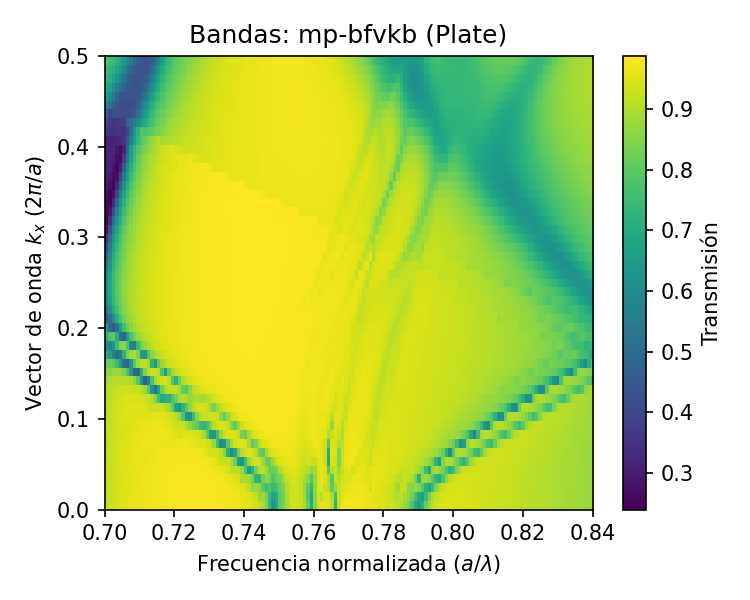
\includegraphics[width=0.48\textwidth]{figures/mp-bfvkb_plate.png}
\hfill
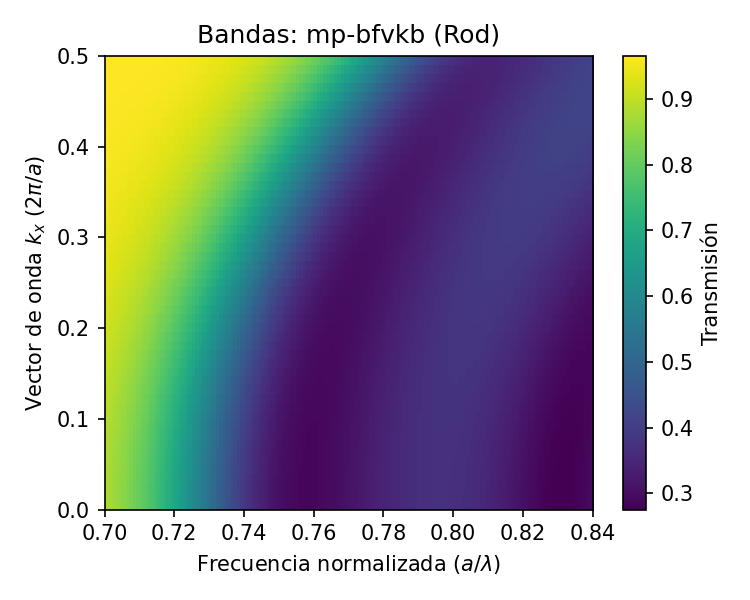
\includegraphics[width=0.48\textwidth]{figures/mp-bfvkb_rod.png}
\caption{Estructuras de bandas fotónicas ($k_x$) para mp-bfvkb. Izquierda: Lámina. Derecha: Cilindros.}
\end{figure}
\vspace{1em}
\begin{figure}[H]
\centering
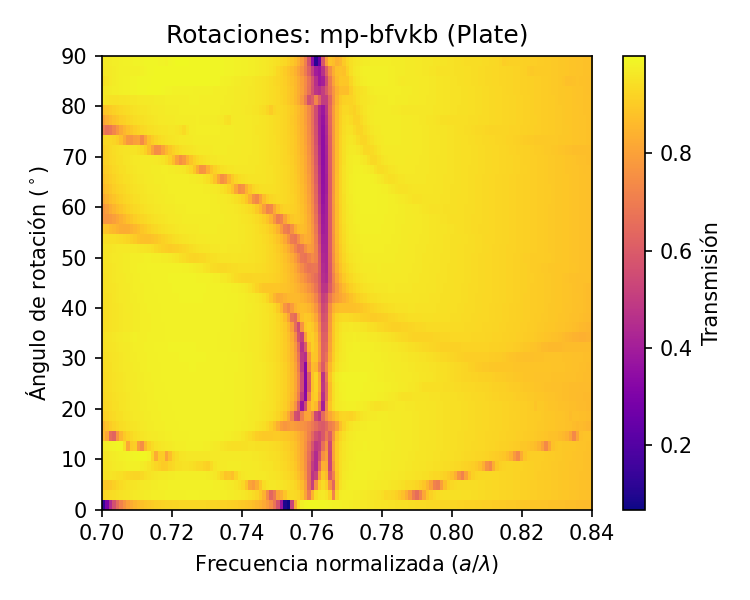
\includegraphics[width=0.48\textwidth]{figures/mp-bfvkb_plate_rangle.png}
\hfill
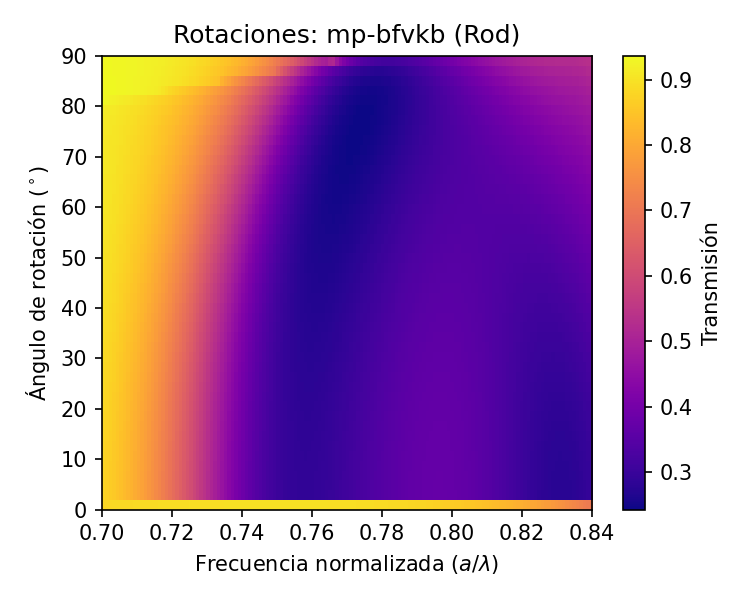
\includegraphics[width=0.48\textwidth]{figures/mp-bfvkb_rod_rangle.png}
\caption{Mapas de transmisión por rotación (twist) para mp-bfvkb. Izquierda: Lámina. Derecha: Cilindros.}
\end{figure}
\vspace{1em}
\hrule
\vspace{1em}
\subsection*{Material ID: mp-bfwfo}
\textbf{Constante Dieléctrica ($\epsilon_{total}$):} 4.46 \\[0.5em]
\begin{table}[h!]
\centering
\begin{tabular}{lcc}
\toprule
\textbf{Métrica} & \textbf{Lámina (Plate)} & \textbf{Cilindros (Rod)} \\
\midrule
Bandgaps ($k_x$) & Ninguno & Ninguno \\
Resonancias ($k_x$) & 36 & 36 \\
\midrule
Bandgaps (Rotación) & Ninguno & Ninguno \\
Resonancias (Rotación) & 33 & 33 \\
\bottomrule
\end{tabular}
\end{table}
\begin{figure}[H]
\centering
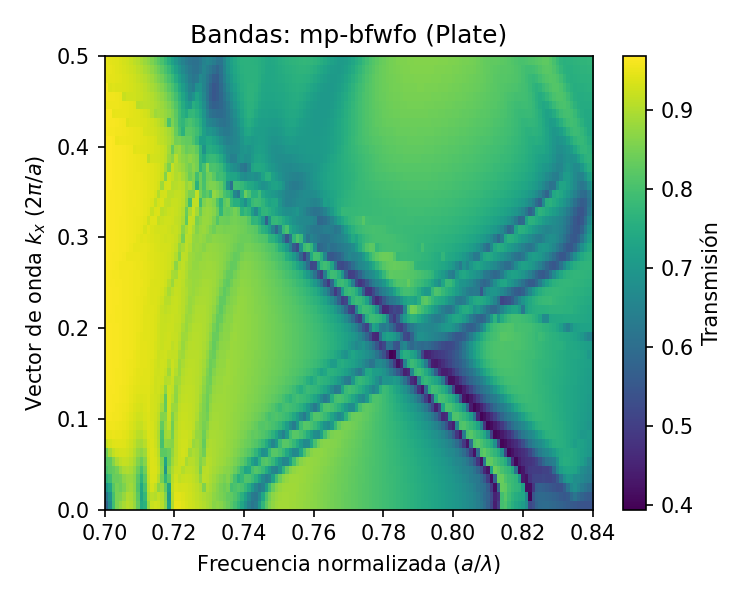
\includegraphics[width=0.48\textwidth]{figures/mp-bfwfo_plate.png}
\hfill
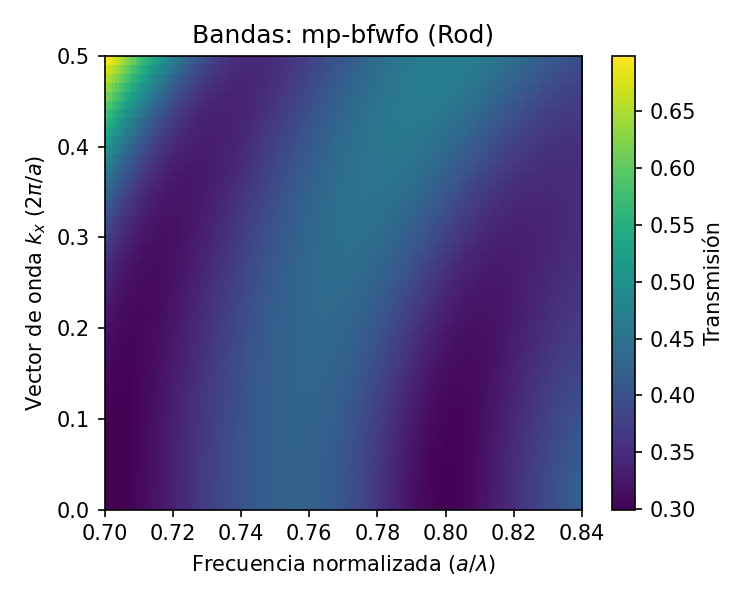
\includegraphics[width=0.48\textwidth]{figures/mp-bfwfo_rod.png}
\caption{Estructuras de bandas fotónicas ($k_x$) para mp-bfwfo. Izquierda: Lámina. Derecha: Cilindros.}
\end{figure}
\vspace{1em}
\begin{figure}[H]
\centering
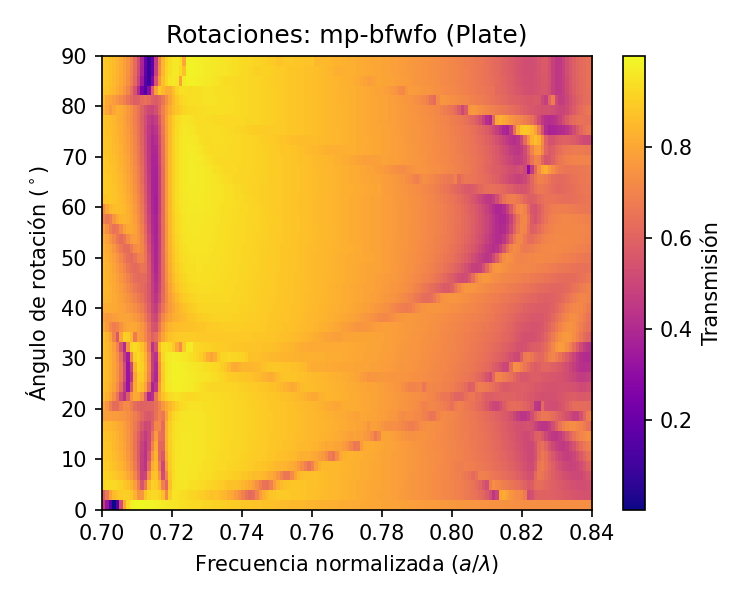
\includegraphics[width=0.48\textwidth]{figures/mp-bfwfo_plate_rangle.png}
\hfill
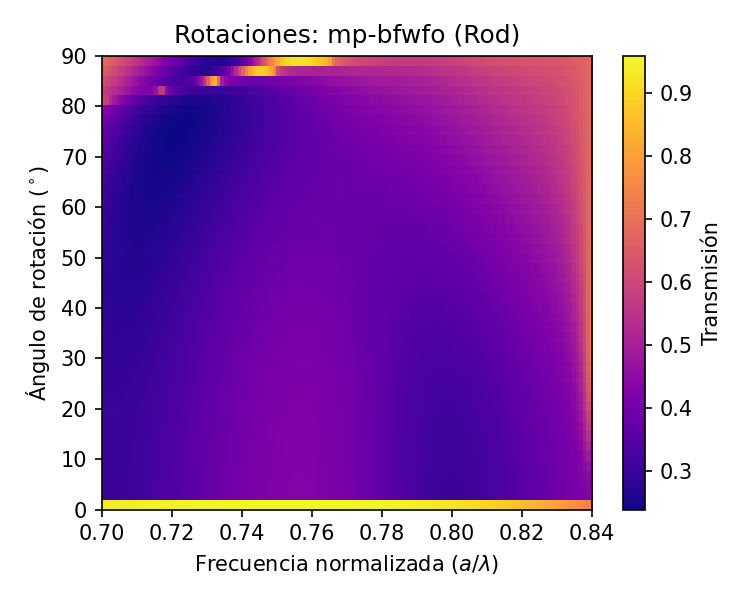
\includegraphics[width=0.48\textwidth]{figures/mp-bfwfo_rod_rangle.png}
\caption{Mapas de transmisión por rotación (twist) para mp-bfwfo. Izquierda: Lámina. Derecha: Cilindros.}
\end{figure}
\vspace{1em}
\hrule
\vspace{1em}
\subsection*{Material ID: mp-bfwhs}
\textbf{Constante Dieléctrica ($\epsilon_{total}$):} 2.99 \\[0.5em]
\begin{table}[h!]
\centering
\begin{tabular}{lcc}
\toprule
\textbf{Métrica} & \textbf{Lámina (Plate)} & \textbf{Cilindros (Rod)} \\
\midrule
Bandgaps ($k_x$) & Ninguno & Ninguno \\
Resonancias ($k_x$) & 36 & 36 \\
\midrule
Bandgaps (Rotación) & Ninguno & Ninguno \\
Resonancias (Rotación) & 33 & 33 \\
\bottomrule
\end{tabular}
\end{table}
\begin{figure}[H]
\centering
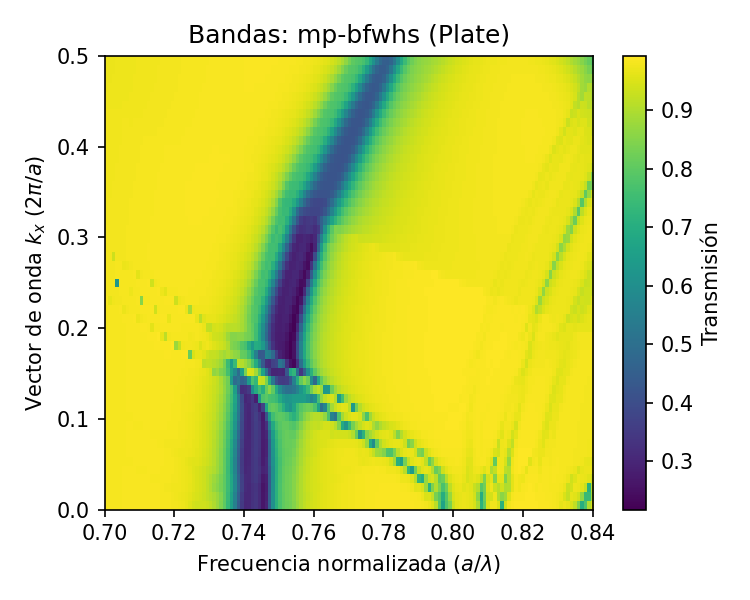
\includegraphics[width=0.48\textwidth]{figures/mp-bfwhs_plate.png}
\hfill
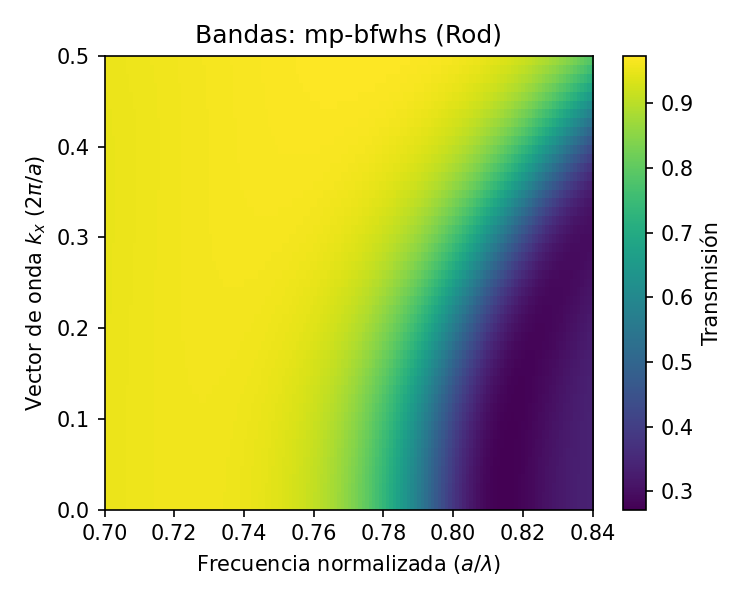
\includegraphics[width=0.48\textwidth]{figures/mp-bfwhs_rod.png}
\caption{Estructuras de bandas fotónicas ($k_x$) para mp-bfwhs. Izquierda: Lámina. Derecha: Cilindros.}
\end{figure}
\vspace{1em}
\begin{figure}[H]
\centering
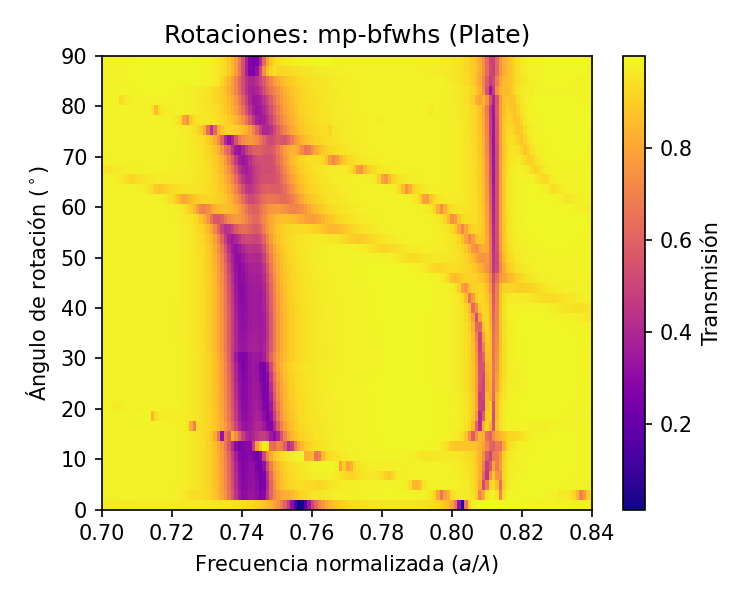
\includegraphics[width=0.48\textwidth]{figures/mp-bfwhs_plate_rangle.png}
\hfill
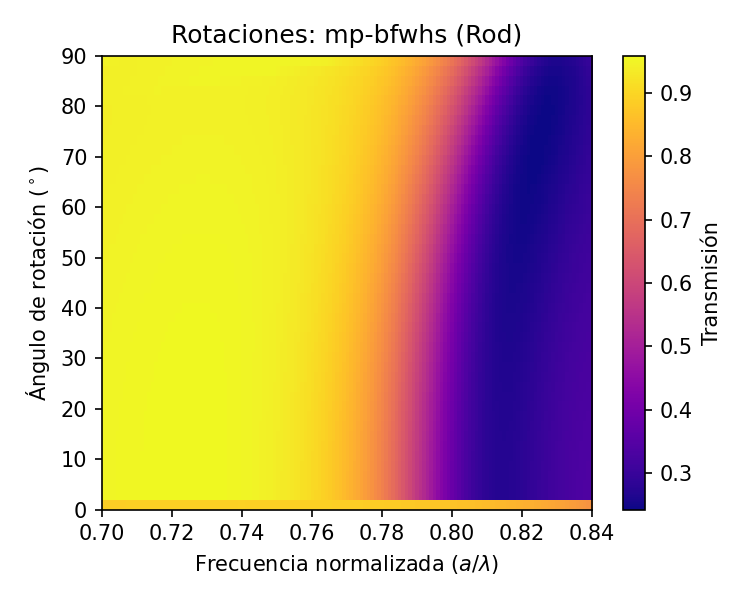
\includegraphics[width=0.48\textwidth]{figures/mp-bfwhs_rod_rangle.png}
\caption{Mapas de transmisión por rotación (twist) para mp-bfwhs. Izquierda: Lámina. Derecha: Cilindros.}
\end{figure}
\vspace{1em}
\hrule
\vspace{1em}
\subsection*{Material ID: mp-bfwsh}
\textbf{Constante Dieléctrica ($\epsilon_{total}$):} 4.84 \\[0.5em]
\begin{table}[h!]
\centering
\begin{tabular}{lcc}
\toprule
\textbf{Métrica} & \textbf{Lámina (Plate)} & \textbf{Cilindros (Rod)} \\
\midrule
Bandgaps ($k_x$) & Ninguno & Ninguno \\
Resonancias ($k_x$) & 36 & 36 \\
\midrule
Bandgaps (Rotación) & Ninguno & Ninguno \\
Resonancias (Rotación) & 33 & 33 \\
\bottomrule
\end{tabular}
\end{table}
\begin{figure}[H]
\centering
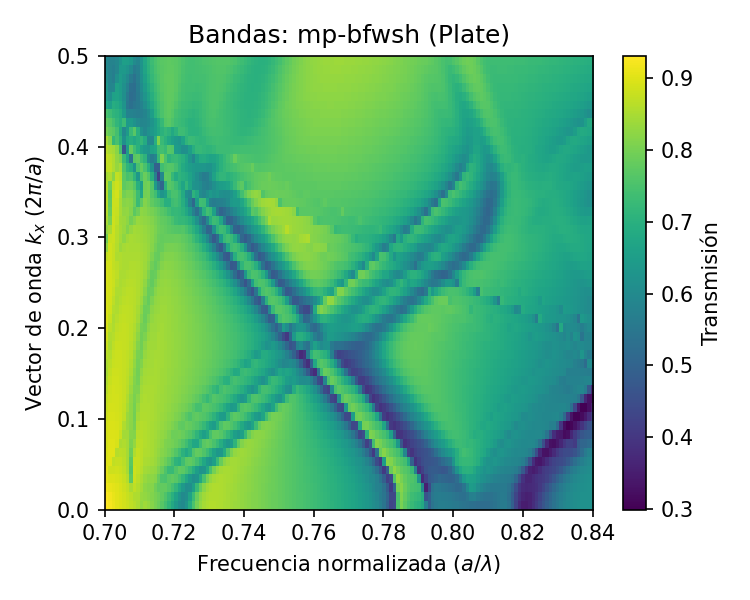
\includegraphics[width=0.48\textwidth]{figures/mp-bfwsh_plate.png}
\hfill
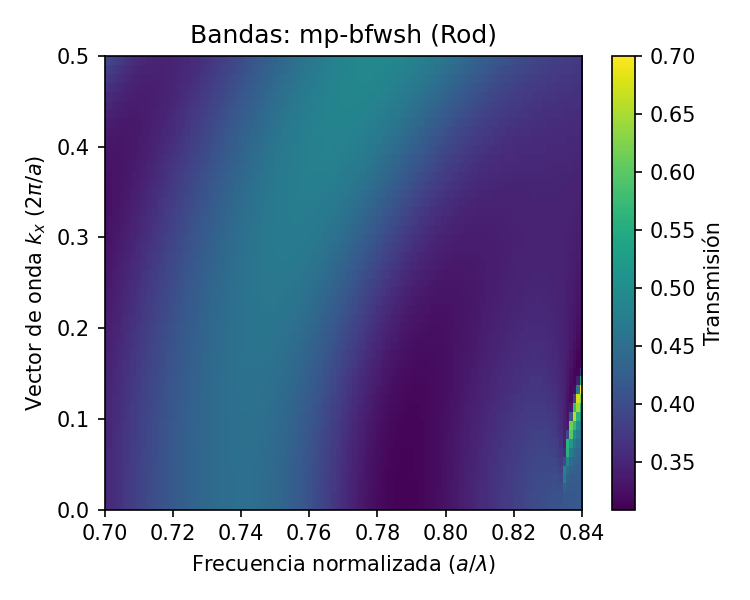
\includegraphics[width=0.48\textwidth]{figures/mp-bfwsh_rod.png}
\caption{Estructuras de bandas fotónicas ($k_x$) para mp-bfwsh. Izquierda: Lámina. Derecha: Cilindros.}
\end{figure}
\vspace{1em}
\begin{figure}[H]
\centering
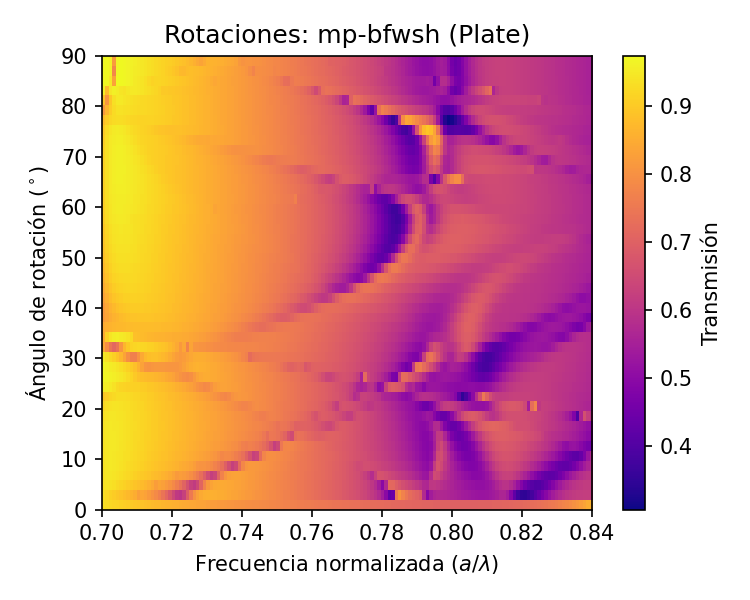
\includegraphics[width=0.48\textwidth]{figures/mp-bfwsh_plate_rangle.png}
\hfill
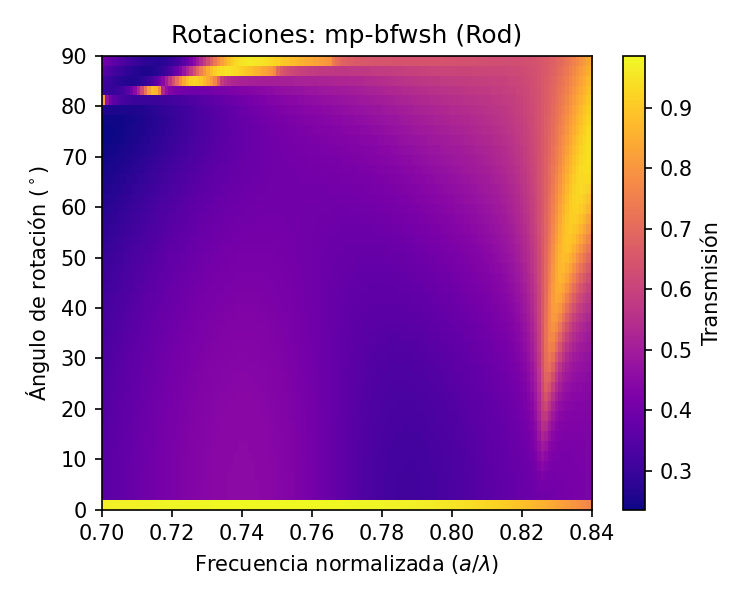
\includegraphics[width=0.48\textwidth]{figures/mp-bfwsh_rod_rangle.png}
\caption{Mapas de transmisión por rotación (twist) para mp-bfwsh. Izquierda: Lámina. Derecha: Cilindros.}
\end{figure}
\vspace{1em}
\hrule
\vspace{1em}
\subsection*{Material ID: mp-bfxet}
\textbf{Constante Dieléctrica ($\epsilon_{total}$):} 3.37 \\[0.5em]
\begin{table}[h!]
\centering
\begin{tabular}{lcc}
\toprule
\textbf{Métrica} & \textbf{Lámina (Plate)} & \textbf{Cilindros (Rod)} \\
\midrule
Bandgaps ($k_x$) & Ninguno & Ninguno \\
Resonancias ($k_x$) & 36 & 36 \\
\midrule
Bandgaps (Rotación) & Ninguno & Ninguno \\
Resonancias (Rotación) & 33 & 33 \\
\bottomrule
\end{tabular}
\end{table}
\begin{figure}[H]
\centering
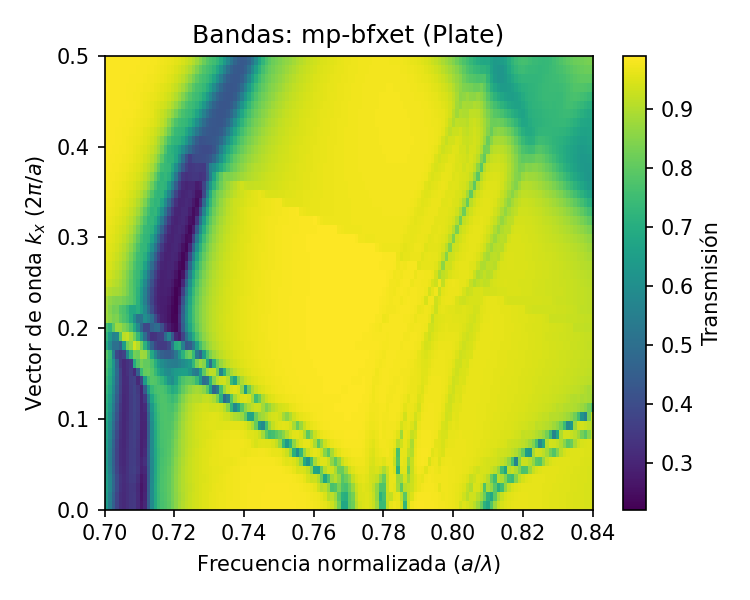
\includegraphics[width=0.48\textwidth]{figures/mp-bfxet_plate.png}
\hfill
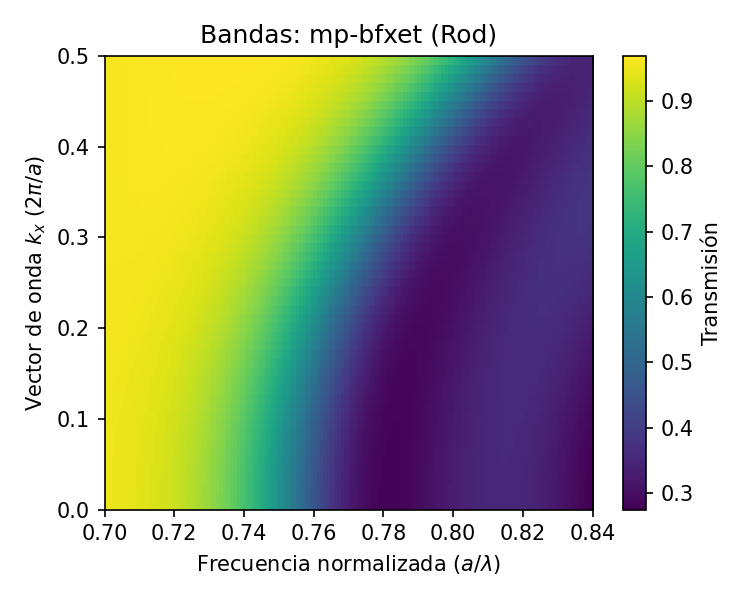
\includegraphics[width=0.48\textwidth]{figures/mp-bfxet_rod.png}
\caption{Estructuras de bandas fotónicas ($k_x$) para mp-bfxet. Izquierda: Lámina. Derecha: Cilindros.}
\end{figure}
\vspace{1em}
\begin{figure}[H]
\centering
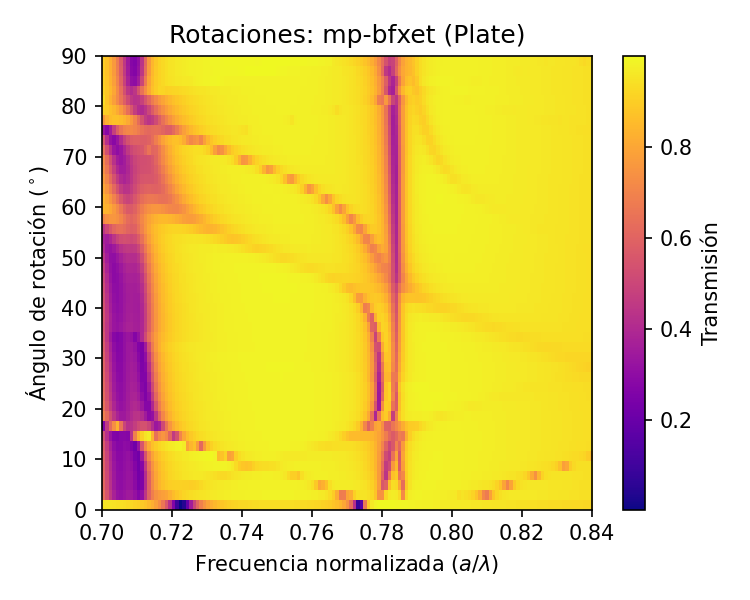
\includegraphics[width=0.48\textwidth]{figures/mp-bfxet_plate_rangle.png}
\hfill
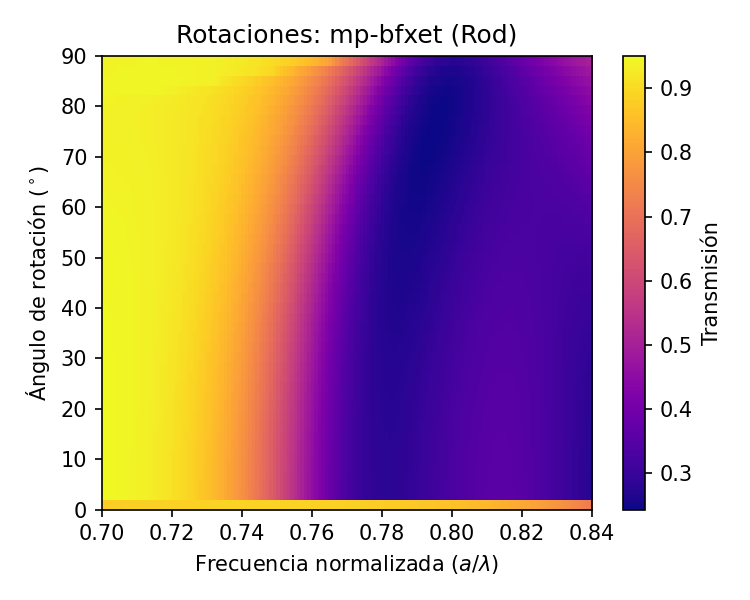
\includegraphics[width=0.48\textwidth]{figures/mp-bfxet_rod_rangle.png}
\caption{Mapas de transmisión por rotación (twist) para mp-bfxet. Izquierda: Lámina. Derecha: Cilindros.}
\end{figure}
\vspace{1em}
\hrule
\vspace{1em}
\subsection*{Material ID: mp-bfxqq}
\textbf{Constante Dieléctrica ($\epsilon_{total}$):} 3.22 \\[0.5em]
\begin{table}[h!]
\centering
\begin{tabular}{lcc}
\toprule
\textbf{Métrica} & \textbf{Lámina (Plate)} & \textbf{Cilindros (Rod)} \\
\midrule
Bandgaps ($k_x$) & Ninguno & Ninguno \\
Resonancias ($k_x$) & 36 & 36 \\
\midrule
Bandgaps (Rotación) & Ninguno & Ninguno \\
Resonancias (Rotación) & 33 & 33 \\
\bottomrule
\end{tabular}
\end{table}
\begin{figure}[H]
\centering
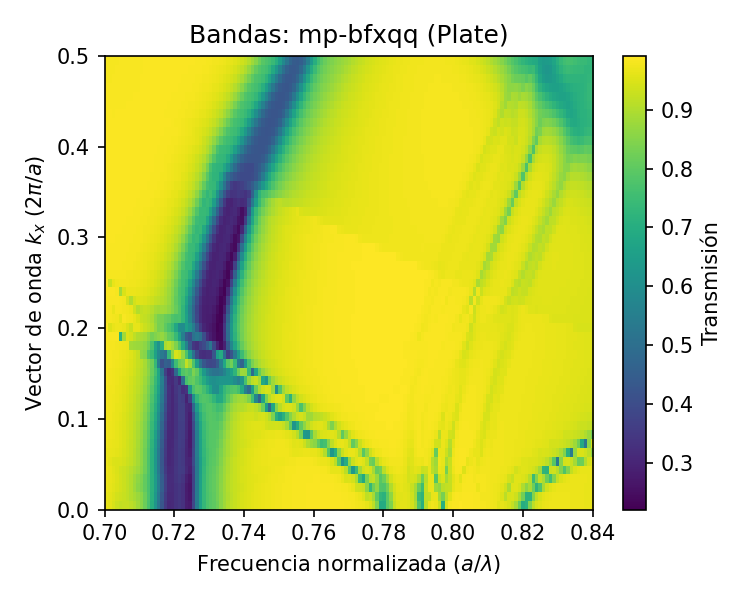
\includegraphics[width=0.48\textwidth]{figures/mp-bfxqq_plate.png}
\hfill
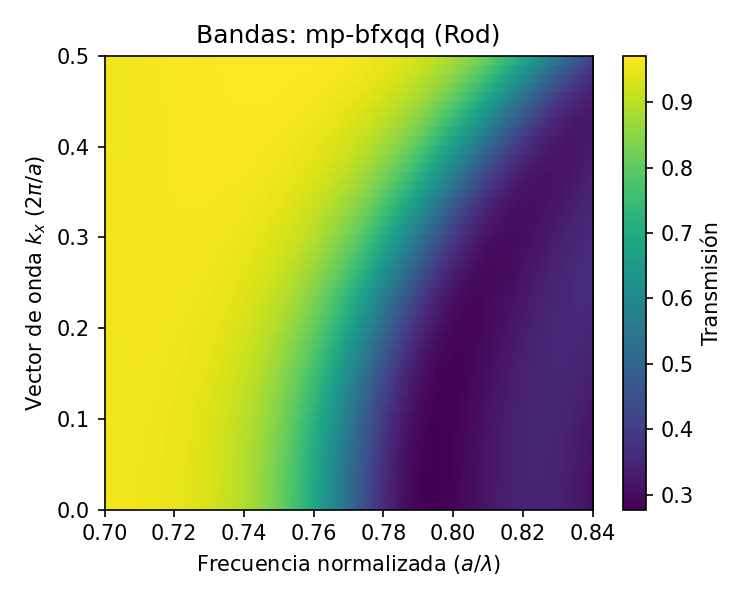
\includegraphics[width=0.48\textwidth]{figures/mp-bfxqq_rod.png}
\caption{Estructuras de bandas fotónicas ($k_x$) para mp-bfxqq. Izquierda: Lámina. Derecha: Cilindros.}
\end{figure}
\vspace{1em}
\begin{figure}[H]
\centering
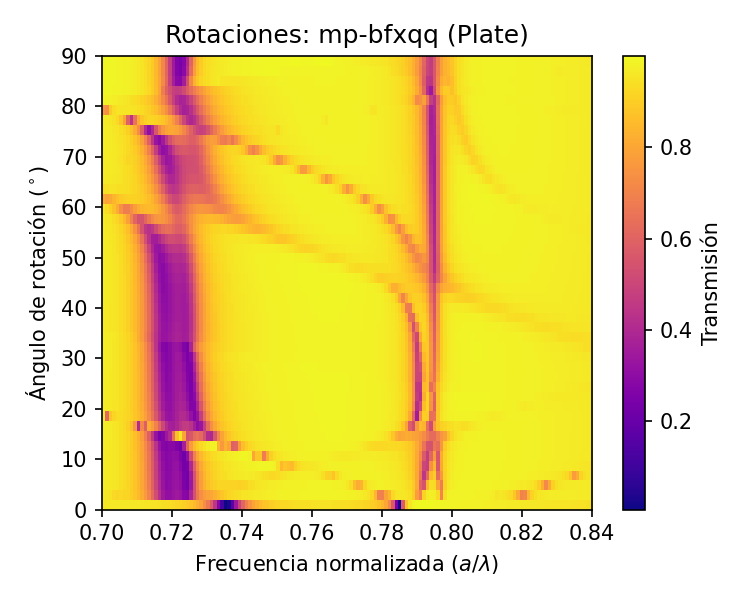
\includegraphics[width=0.48\textwidth]{figures/mp-bfxqq_plate_rangle.png}
\hfill
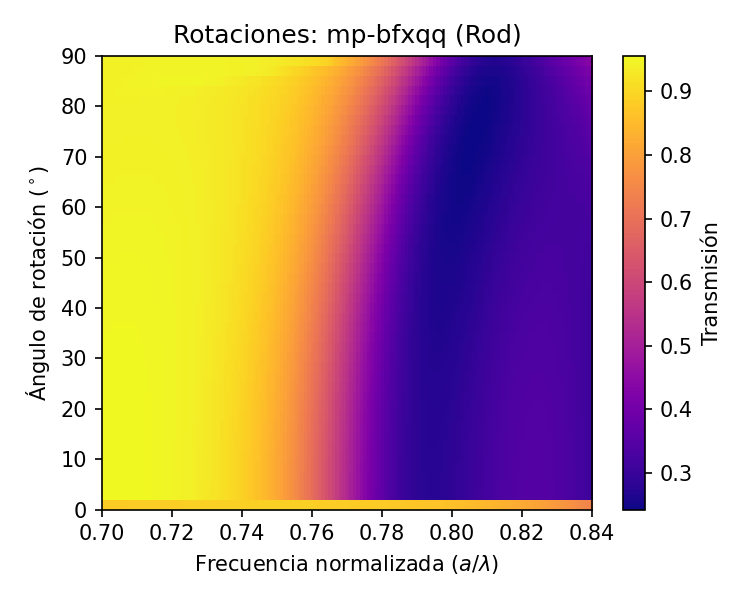
\includegraphics[width=0.48\textwidth]{figures/mp-bfxqq_rod_rangle.png}
\caption{Mapas de transmisión por rotación (twist) para mp-bfxqq. Izquierda: Lámina. Derecha: Cilindros.}
\end{figure}
\vspace{1em}
\hrule
\vspace{1em}
\subsection*{Material ID: mp-bfyid}
\textbf{Constante Dieléctrica ($\epsilon_{total}$):} 4.33 \\[0.5em]
\begin{table}[h!]
\centering
\begin{tabular}{lcc}
\toprule
\textbf{Métrica} & \textbf{Lámina (Plate)} & \textbf{Cilindros (Rod)} \\
\midrule
Bandgaps ($k_x$) & Ninguno & Ninguno \\
Resonancias ($k_x$) & 36 & 36 \\
\midrule
Bandgaps (Rotación) & Ninguno & Ninguno \\
Resonancias (Rotación) & 33 & 33 \\
\bottomrule
\end{tabular}
\end{table}
\begin{figure}[H]
\centering
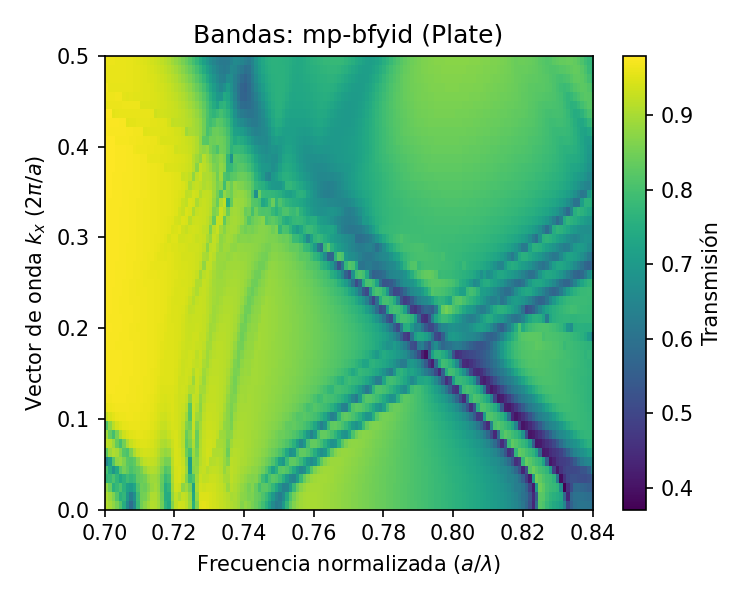
\includegraphics[width=0.48\textwidth]{figures/mp-bfyid_plate.png}
\hfill
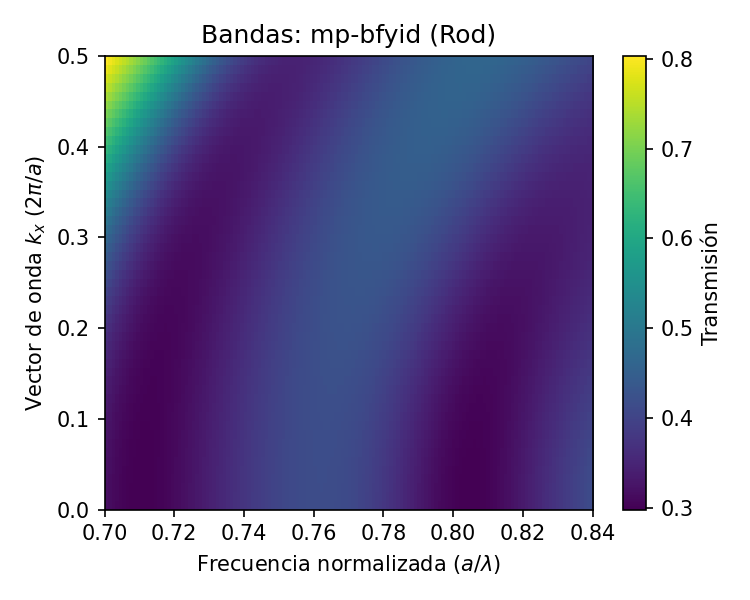
\includegraphics[width=0.48\textwidth]{figures/mp-bfyid_rod.png}
\caption{Estructuras de bandas fotónicas ($k_x$) para mp-bfyid. Izquierda: Lámina. Derecha: Cilindros.}
\end{figure}
\vspace{1em}
\begin{figure}[H]
\centering
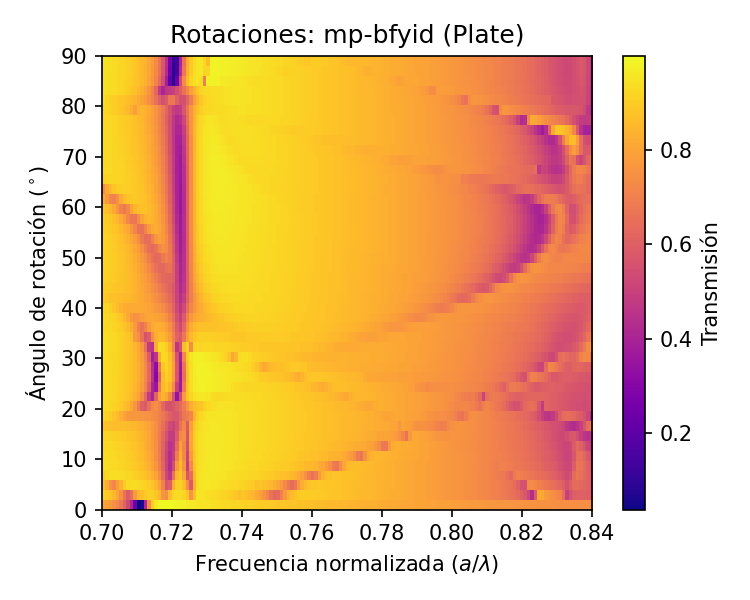
\includegraphics[width=0.48\textwidth]{figures/mp-bfyid_plate_rangle.png}
\hfill
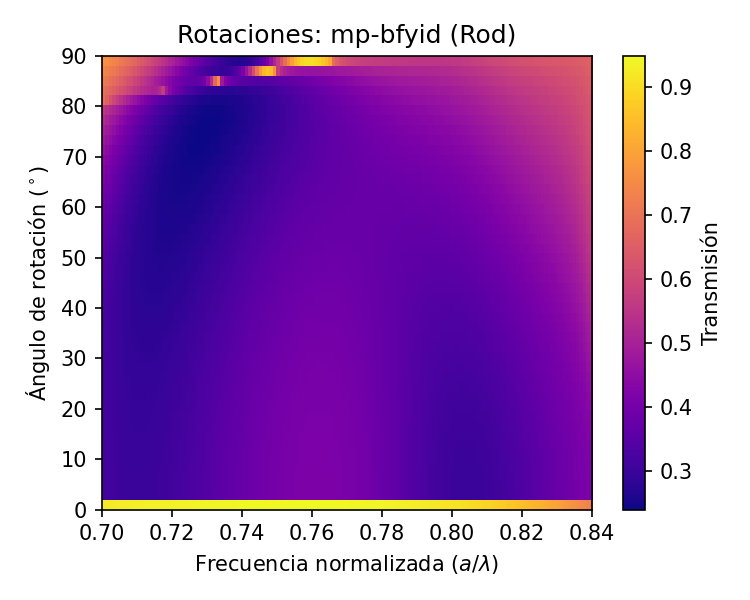
\includegraphics[width=0.48\textwidth]{figures/mp-bfyid_rod_rangle.png}
\caption{Mapas de transmisión por rotación (twist) para mp-bfyid. Izquierda: Lámina. Derecha: Cilindros.}
\end{figure}
\vspace{1em}
\hrule
\vspace{1em}
\subsection*{Material ID: mp-bidoy}
\textbf{Constante Dieléctrica ($\epsilon_{total}$):} 3.33 \\[0.5em]
\begin{table}[h!]
\centering
\begin{tabular}{lcc}
\toprule
\textbf{Métrica} & \textbf{Lámina (Plate)} & \textbf{Cilindros (Rod)} \\
\midrule
Bandgaps ($k_x$) & Ninguno & Ninguno \\
Resonancias ($k_x$) & 36 & 36 \\
\midrule
Bandgaps (Rotación) & Ninguno & Ninguno \\
Resonancias (Rotación) & 33 & 33 \\
\bottomrule
\end{tabular}
\end{table}
\begin{figure}[H]
\centering
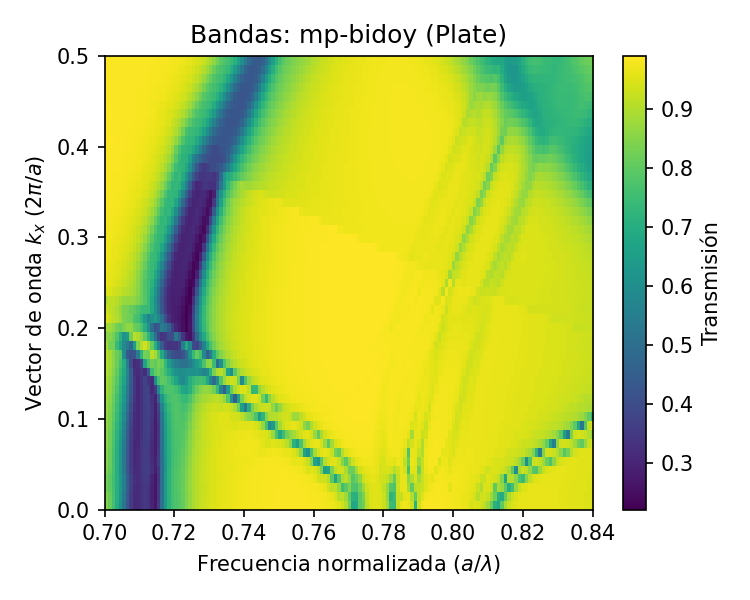
\includegraphics[width=0.48\textwidth]{figures/mp-bidoy_plate.png}
\hfill
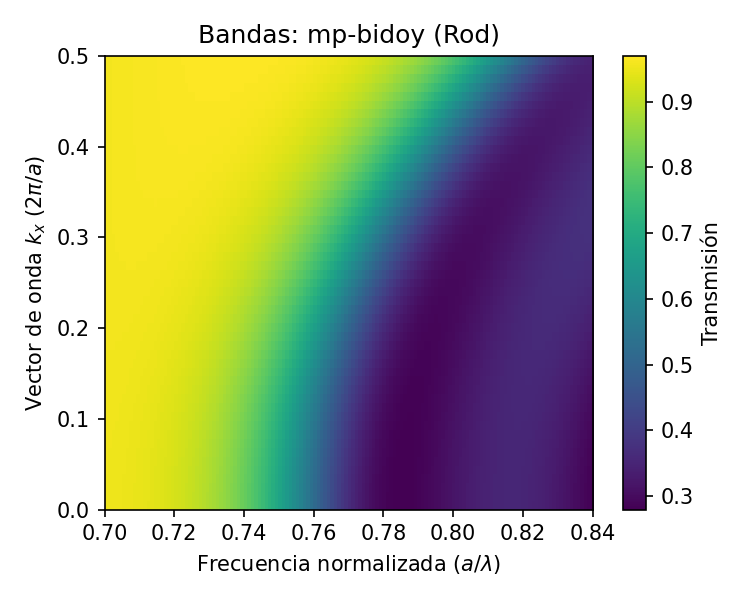
\includegraphics[width=0.48\textwidth]{figures/mp-bidoy_rod.png}
\caption{Estructuras de bandas fotónicas ($k_x$) para mp-bidoy. Izquierda: Lámina. Derecha: Cilindros.}
\end{figure}
\vspace{1em}
\begin{figure}[H]
\centering
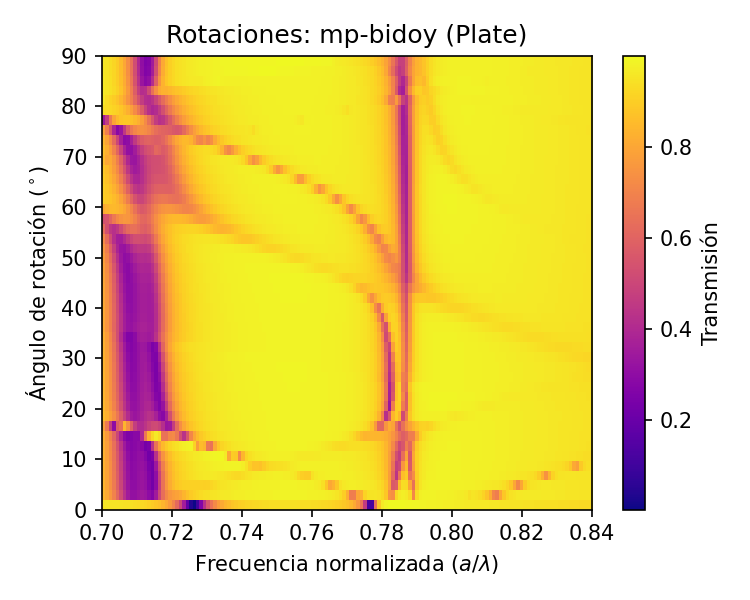
\includegraphics[width=0.48\textwidth]{figures/mp-bidoy_plate_rangle.png}
\hfill
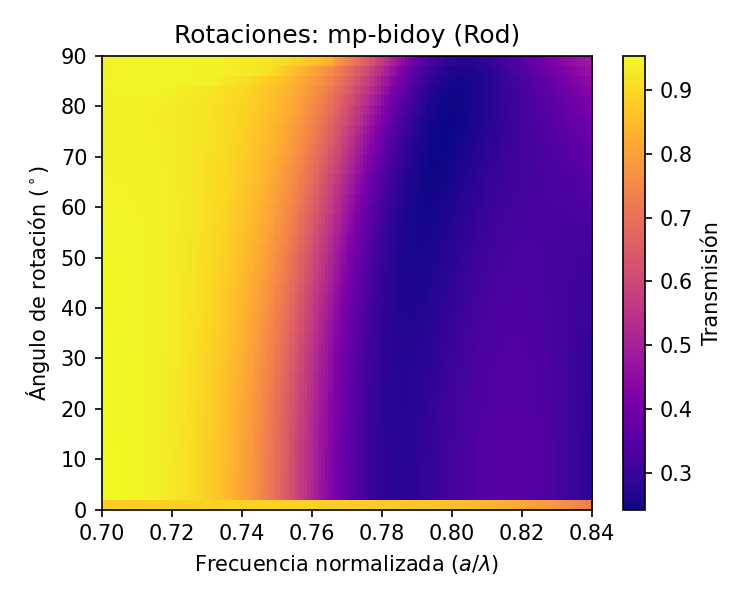
\includegraphics[width=0.48\textwidth]{figures/mp-bidoy_rod_rangle.png}
\caption{Mapas de transmisión por rotación (twist) para mp-bidoy. Izquierda: Lámina. Derecha: Cilindros.}
\end{figure}
\vspace{1em}
\hrule
\vspace{1em}
\subsection*{Material ID: mp-bidoz}
\textbf{Constante Dieléctrica ($\epsilon_{total}$):} 3.00 \\[0.5em]
\begin{table}[h!]
\centering
\begin{tabular}{lcc}
\toprule
\textbf{Métrica} & \textbf{Lámina (Plate)} & \textbf{Cilindros (Rod)} \\
\midrule
Bandgaps ($k_x$) & Ninguno & Ninguno \\
Resonancias ($k_x$) & 36 & 36 \\
\midrule
Bandgaps (Rotación) & Ninguno & Ninguno \\
Resonancias (Rotación) & 33 & 33 \\
\bottomrule
\end{tabular}
\end{table}
\begin{figure}[H]
\centering
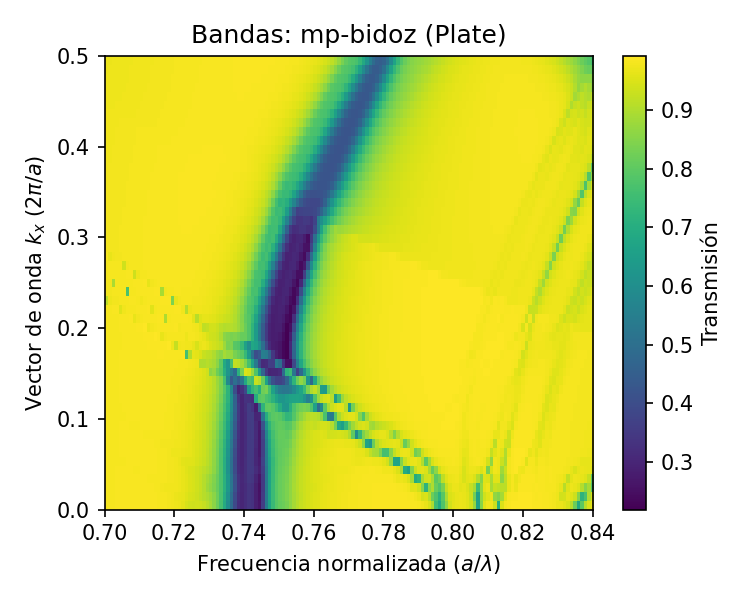
\includegraphics[width=0.48\textwidth]{figures/mp-bidoz_plate.png}
\hfill
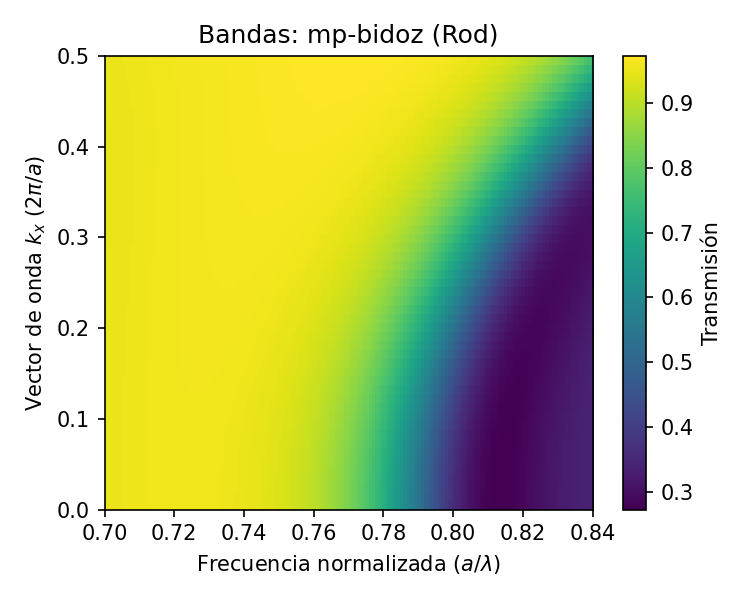
\includegraphics[width=0.48\textwidth]{figures/mp-bidoz_rod.png}
\caption{Estructuras de bandas fotónicas ($k_x$) para mp-bidoz. Izquierda: Lámina. Derecha: Cilindros.}
\end{figure}
\vspace{1em}
\begin{figure}[H]
\centering
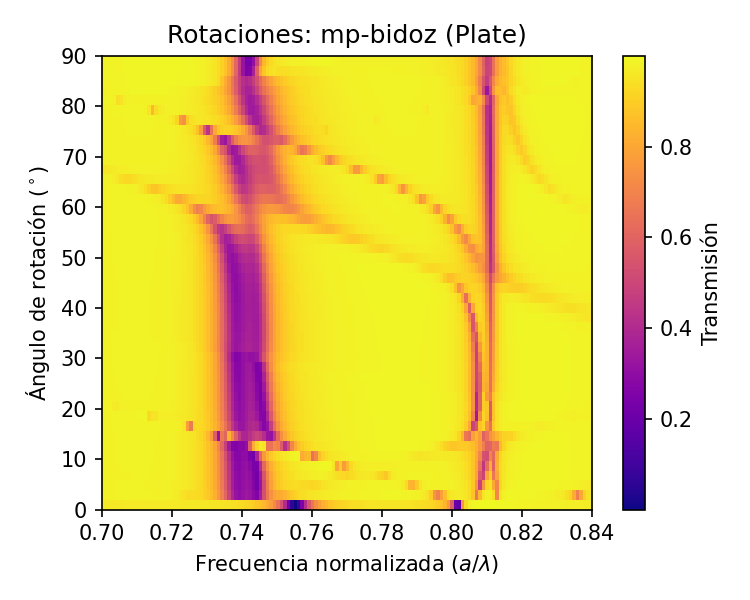
\includegraphics[width=0.48\textwidth]{figures/mp-bidoz_plate_rangle.png}
\hfill
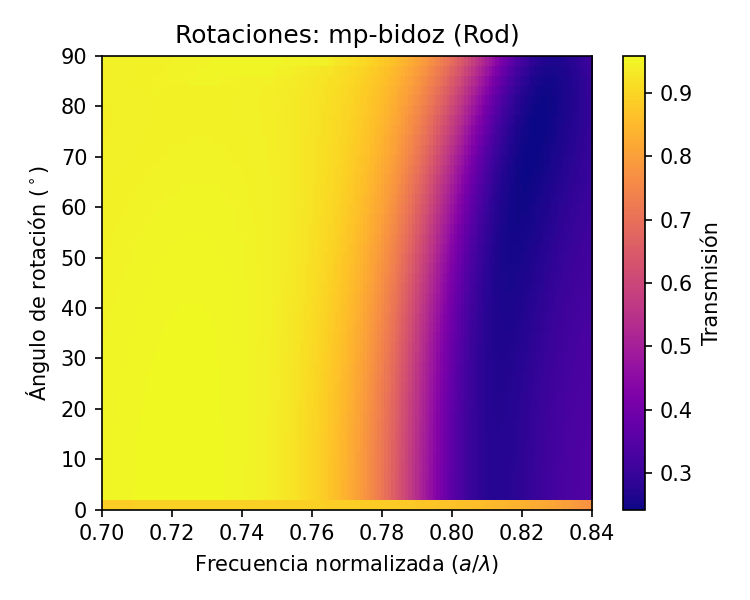
\includegraphics[width=0.48\textwidth]{figures/mp-bidoz_rod_rangle.png}
\caption{Mapas de transmisión por rotación (twist) para mp-bidoz. Izquierda: Lámina. Derecha: Cilindros.}
\end{figure}
\vspace{1em}
\hrule
\vspace{1em}
\subsection*{Material ID: mp-bidpa}
\textbf{Constante Dieléctrica ($\epsilon_{total}$):} 3.33 \\[0.5em]
\begin{table}[h!]
\centering
\begin{tabular}{lcc}
\toprule
\textbf{Métrica} & \textbf{Lámina (Plate)} & \textbf{Cilindros (Rod)} \\
\midrule
Bandgaps ($k_x$) & Ninguno & Ninguno \\
Resonancias ($k_x$) & 36 & 36 \\
\midrule
Bandgaps (Rotación) & Ninguno & Ninguno \\
Resonancias (Rotación) & 33 & 33 \\
\bottomrule
\end{tabular}
\end{table}
\begin{figure}[H]
\centering
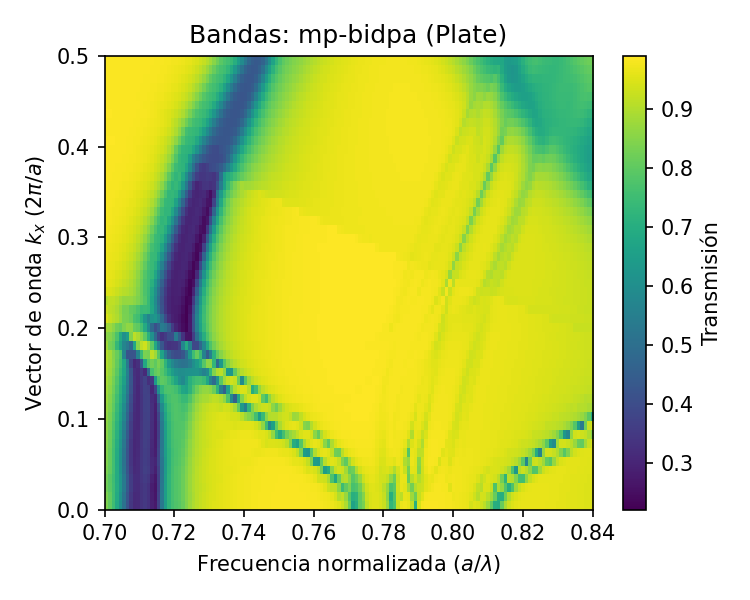
\includegraphics[width=0.48\textwidth]{figures/mp-bidpa_plate.png}
\hfill
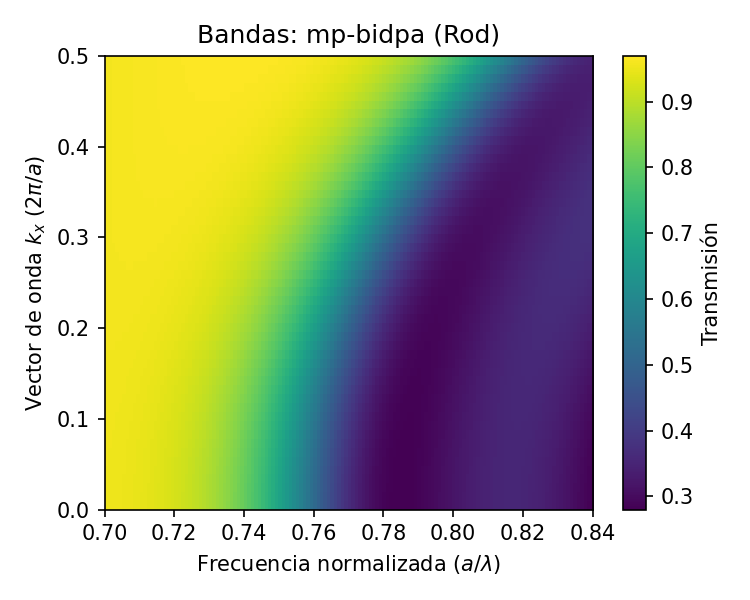
\includegraphics[width=0.48\textwidth]{figures/mp-bidpa_rod.png}
\caption{Estructuras de bandas fotónicas ($k_x$) para mp-bidpa. Izquierda: Lámina. Derecha: Cilindros.}
\end{figure}
\vspace{1em}
\begin{figure}[H]
\centering
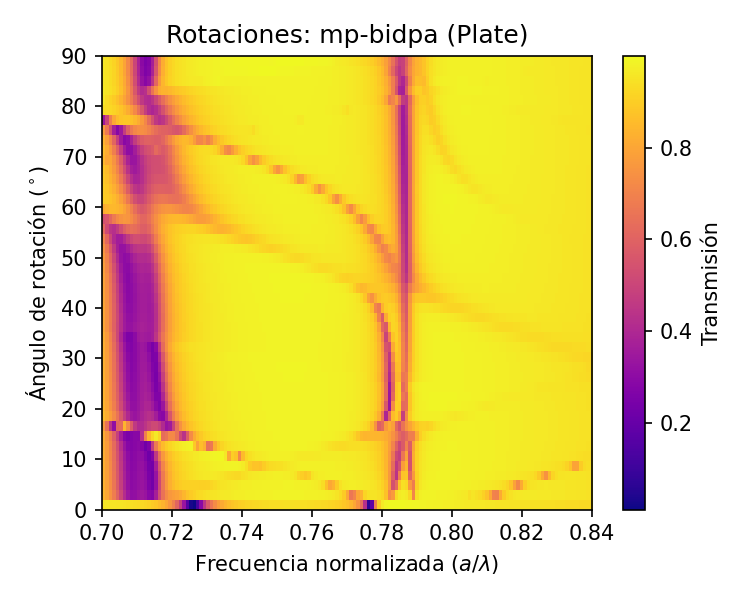
\includegraphics[width=0.48\textwidth]{figures/mp-bidpa_plate_rangle.png}
\hfill
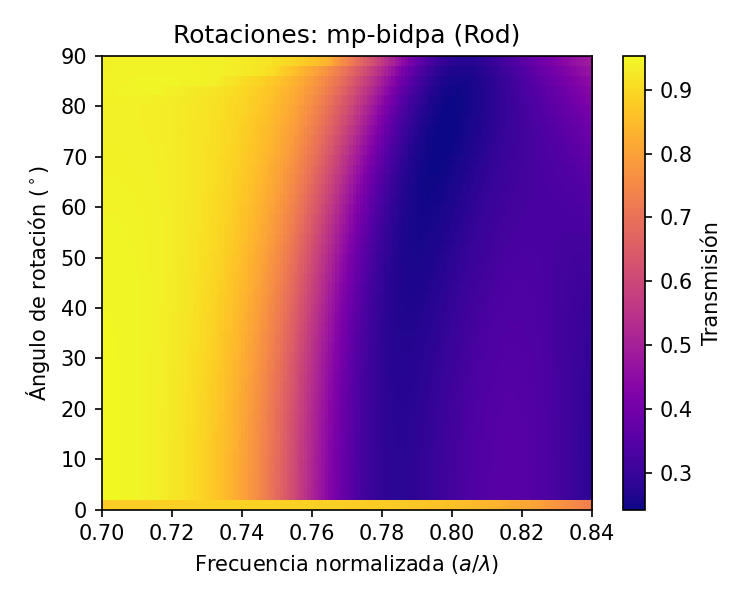
\includegraphics[width=0.48\textwidth]{figures/mp-bidpa_rod_rangle.png}
\caption{Mapas de transmisión por rotación (twist) para mp-bidpa. Izquierda: Lámina. Derecha: Cilindros.}
\end{figure}
\vspace{1em}
\hrule
\vspace{1em}
\subsection*{Material ID: mp-bidpc}
\textbf{Constante Dieléctrica ($\epsilon_{total}$):} 3.61 \\[0.5em]
\begin{table}[h!]
\centering
\begin{tabular}{lcc}
\toprule
\textbf{Métrica} & \textbf{Lámina (Plate)} & \textbf{Cilindros (Rod)} \\
\midrule
Bandgaps ($k_x$) & Ninguno & Ninguno \\
Resonancias ($k_x$) & 36 & 36 \\
\midrule
Bandgaps (Rotación) & Ninguno & Ninguno \\
Resonancias (Rotación) & 33 & 33 \\
\bottomrule
\end{tabular}
\end{table}
\begin{figure}[H]
\centering
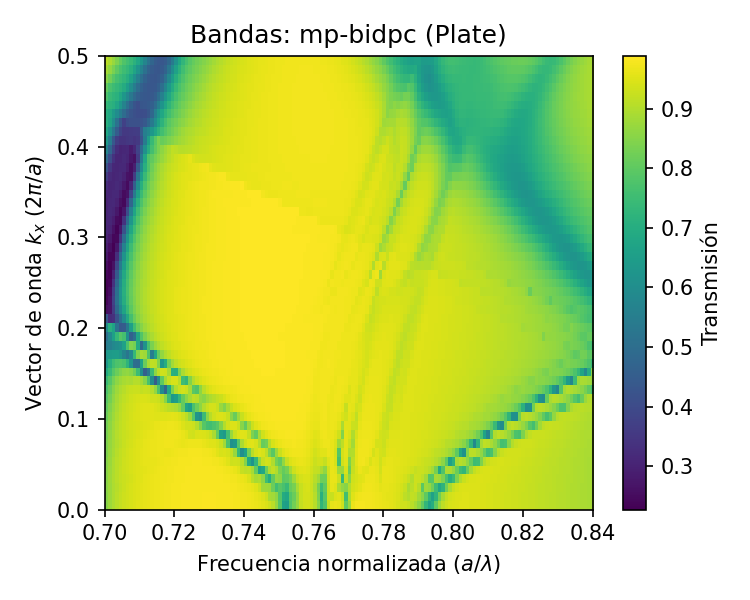
\includegraphics[width=0.48\textwidth]{figures/mp-bidpc_plate.png}
\hfill
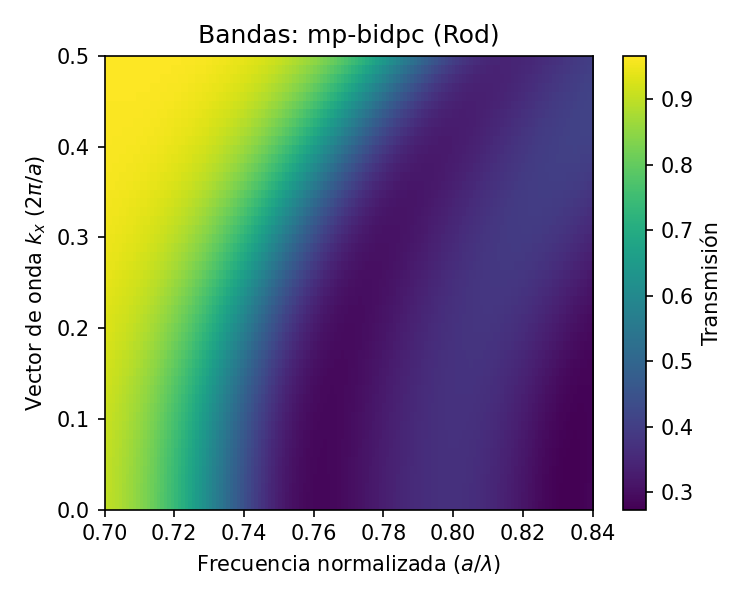
\includegraphics[width=0.48\textwidth]{figures/mp-bidpc_rod.png}
\caption{Estructuras de bandas fotónicas ($k_x$) para mp-bidpc. Izquierda: Lámina. Derecha: Cilindros.}
\end{figure}
\vspace{1em}
\begin{figure}[H]
\centering
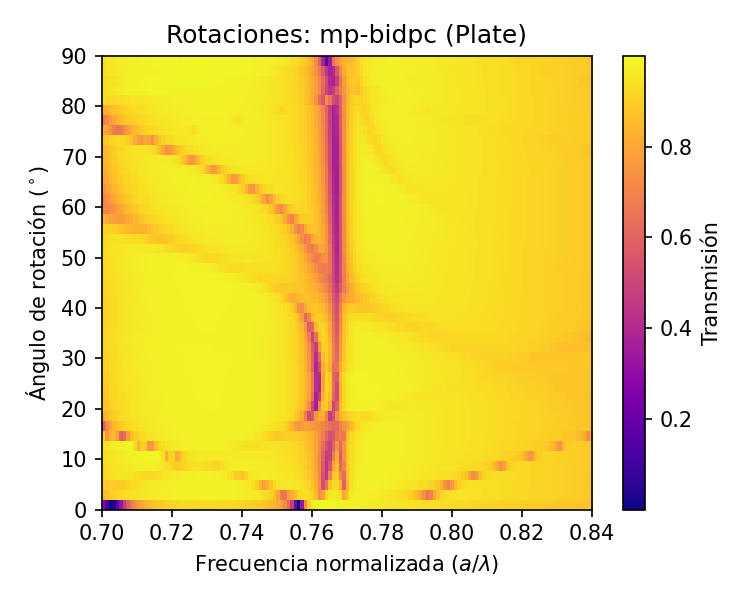
\includegraphics[width=0.48\textwidth]{figures/mp-bidpc_plate_rangle.png}
\hfill
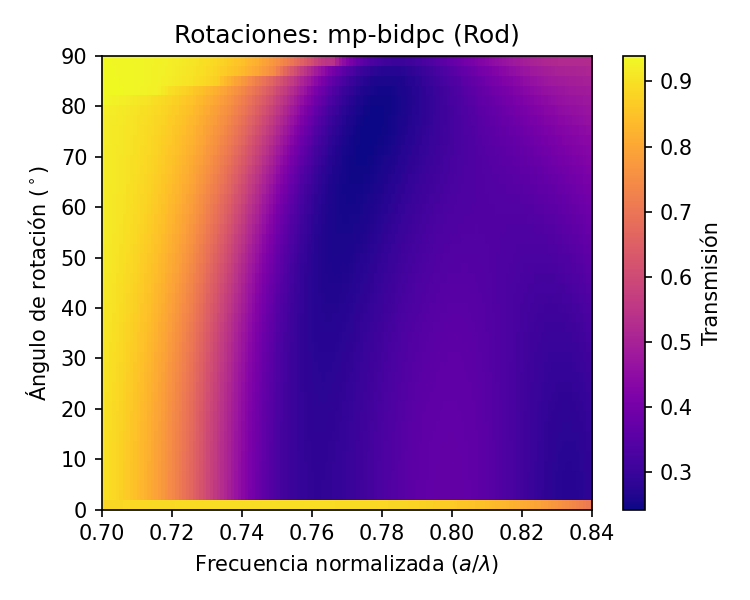
\includegraphics[width=0.48\textwidth]{figures/mp-bidpc_rod_rangle.png}
\caption{Mapas de transmisión por rotación (twist) para mp-bidpc. Izquierda: Lámina. Derecha: Cilindros.}
\end{figure}
\vspace{1em}
\hrule
\vspace{1em}
\subsection*{Material ID: mp-bidqf}
\textbf{Constante Dieléctrica ($\epsilon_{total}$):} 3.23 \\[0.5em]
\begin{table}[h!]
\centering
\begin{tabular}{lcc}
\toprule
\textbf{Métrica} & \textbf{Lámina (Plate)} & \textbf{Cilindros (Rod)} \\
\midrule
Bandgaps ($k_x$) & Ninguno & Ninguno \\
Resonancias ($k_x$) & 36 & 36 \\
\midrule
Bandgaps (Rotación) & Ninguno & Ninguno \\
Resonancias (Rotación) & 33 & 33 \\
\bottomrule
\end{tabular}
\end{table}
\begin{figure}[H]
\centering
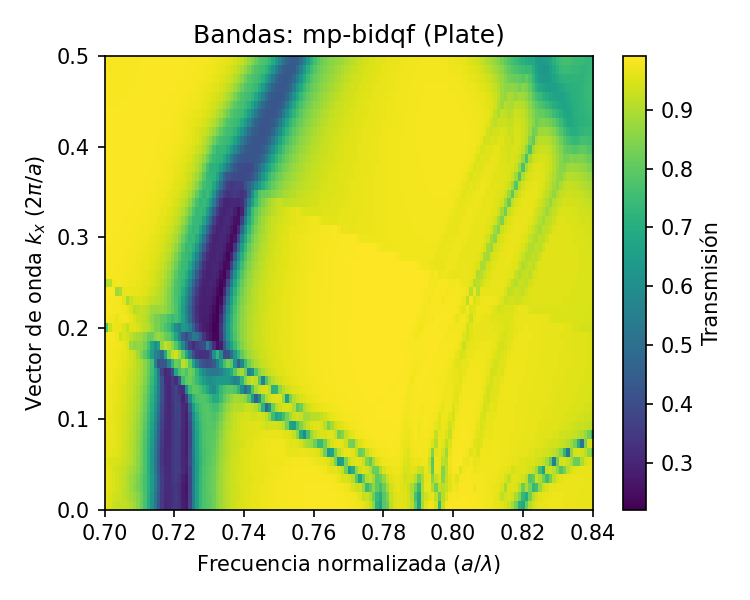
\includegraphics[width=0.48\textwidth]{figures/mp-bidqf_plate.png}
\hfill
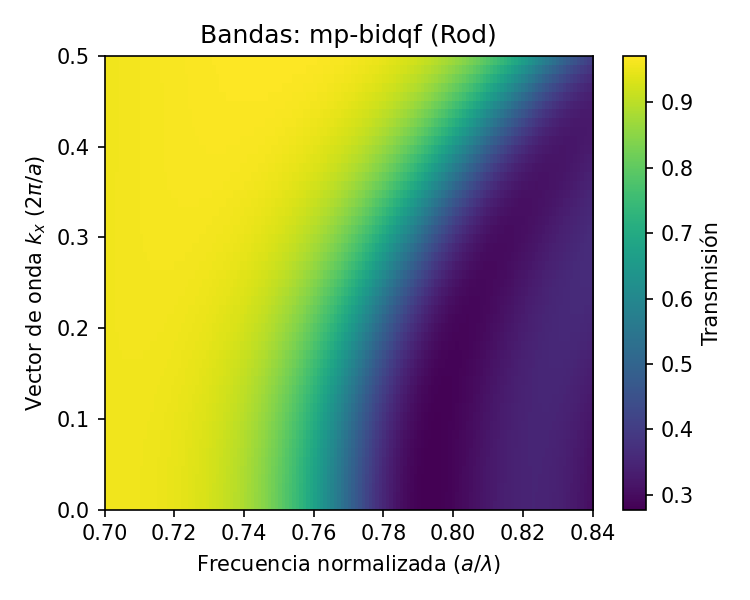
\includegraphics[width=0.48\textwidth]{figures/mp-bidqf_rod.png}
\caption{Estructuras de bandas fotónicas ($k_x$) para mp-bidqf. Izquierda: Lámina. Derecha: Cilindros.}
\end{figure}
\vspace{1em}
\begin{figure}[H]
\centering
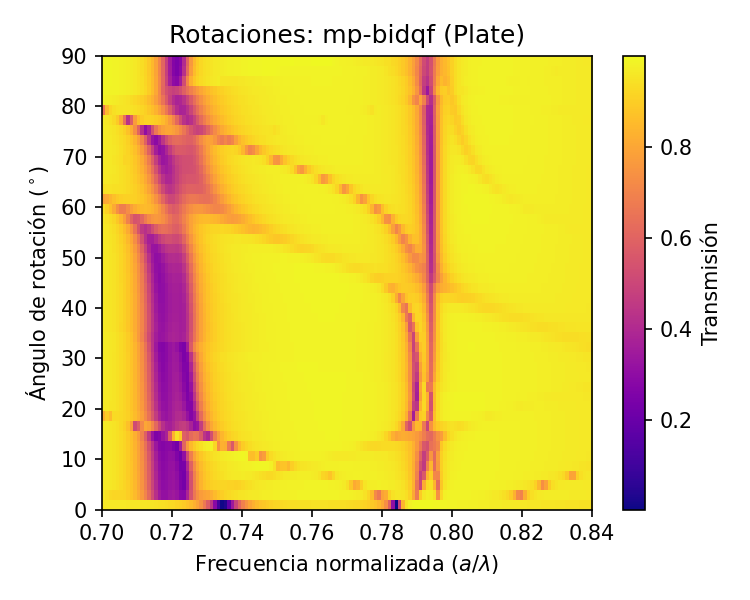
\includegraphics[width=0.48\textwidth]{figures/mp-bidqf_plate_rangle.png}
\hfill
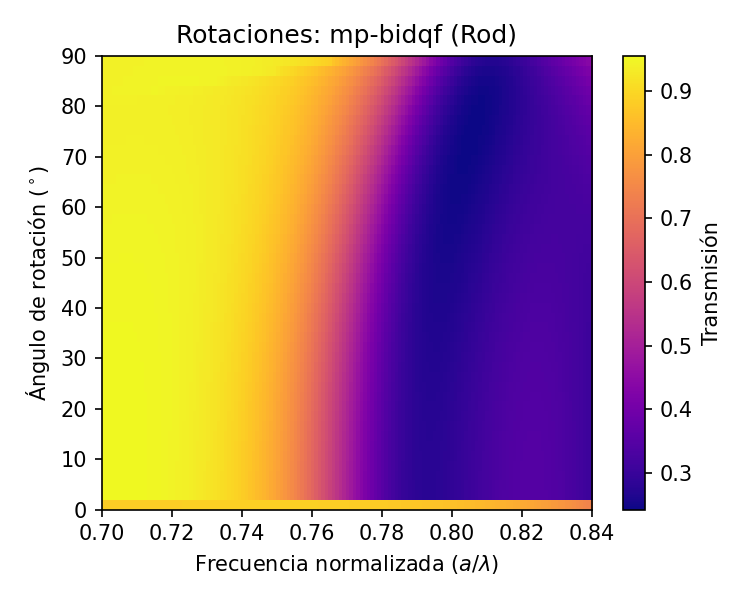
\includegraphics[width=0.48\textwidth]{figures/mp-bidqf_rod_rangle.png}
\caption{Mapas de transmisión por rotación (twist) para mp-bidqf. Izquierda: Lámina. Derecha: Cilindros.}
\end{figure}
\vspace{1em}
\hrule
\vspace{1em}
\subsection*{Material ID: mp-bidqk}
\textbf{Constante Dieléctrica ($\epsilon_{total}$):} 3.00 \\[0.5em]
\begin{table}[h!]
\centering
\begin{tabular}{lcc}
\toprule
\textbf{Métrica} & \textbf{Lámina (Plate)} & \textbf{Cilindros (Rod)} \\
\midrule
Bandgaps ($k_x$) & Ninguno & Ninguno \\
Resonancias ($k_x$) & 36 & 36 \\
\midrule
Bandgaps (Rotación) & Ninguno & Ninguno \\
Resonancias (Rotación) & 33 & 33 \\
\bottomrule
\end{tabular}
\end{table}
\begin{figure}[H]
\centering
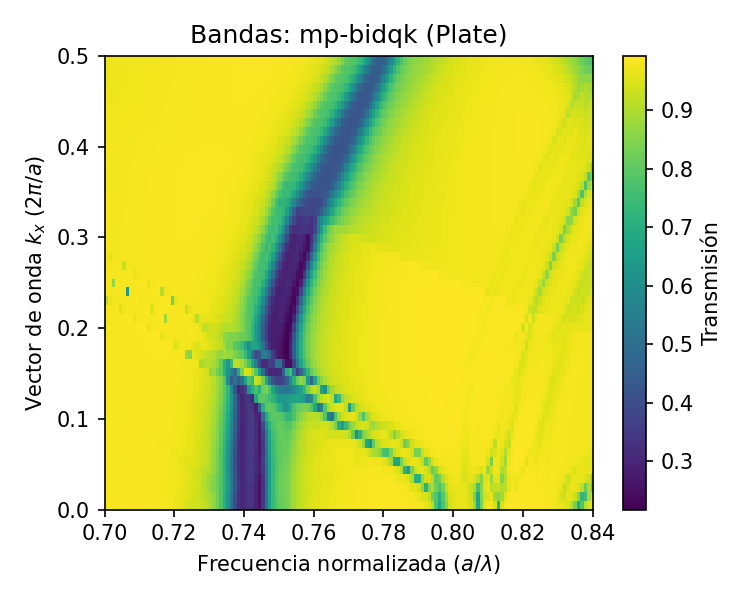
\includegraphics[width=0.48\textwidth]{figures/mp-bidqk_plate.png}
\hfill
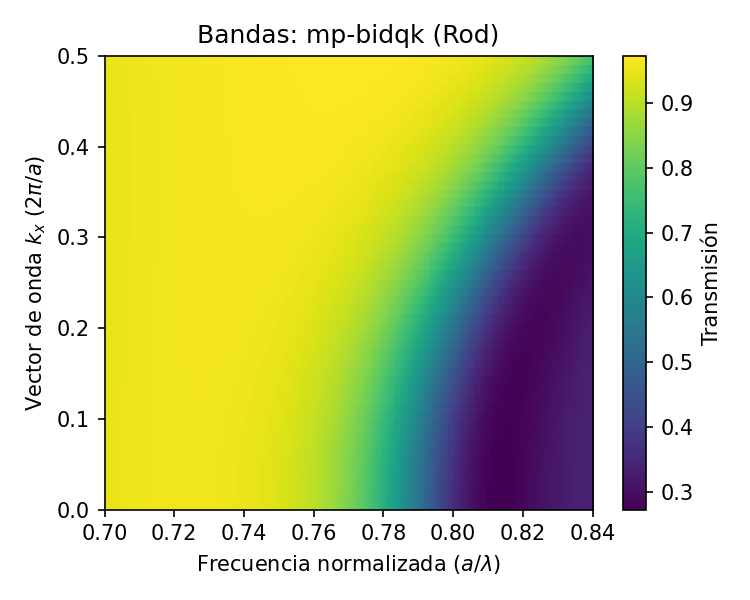
\includegraphics[width=0.48\textwidth]{figures/mp-bidqk_rod.png}
\caption{Estructuras de bandas fotónicas ($k_x$) para mp-bidqk. Izquierda: Lámina. Derecha: Cilindros.}
\end{figure}
\vspace{1em}
\begin{figure}[H]
\centering
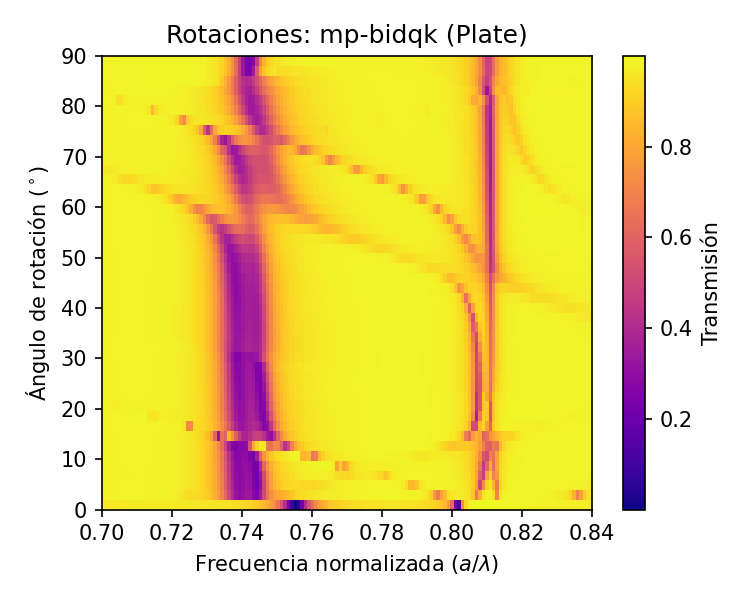
\includegraphics[width=0.48\textwidth]{figures/mp-bidqk_plate_rangle.png}
\hfill
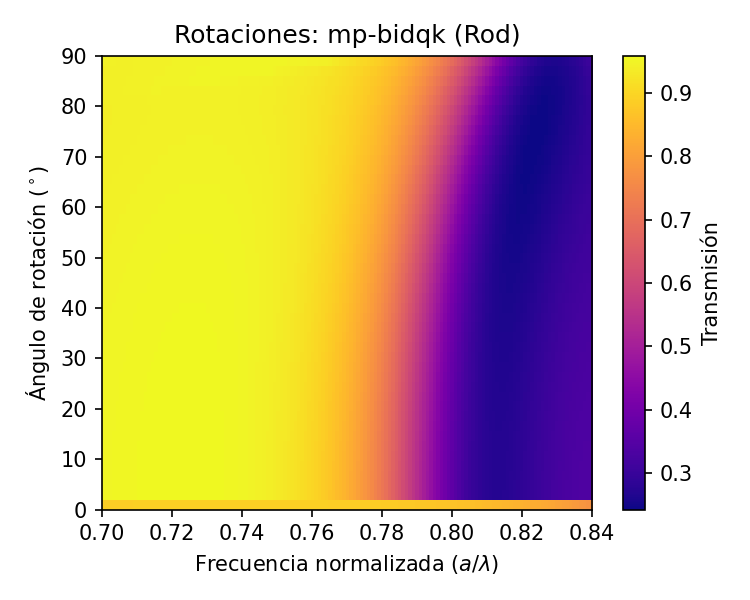
\includegraphics[width=0.48\textwidth]{figures/mp-bidqk_rod_rangle.png}
\caption{Mapas de transmisión por rotación (twist) para mp-bidqk. Izquierda: Lámina. Derecha: Cilindros.}
\end{figure}
\vspace{1em}
\hrule
\vspace{1em}
\subsection*{Material ID: mp-bidrf}
\textbf{Constante Dieléctrica ($\epsilon_{total}$):} 3.58 \\[0.5em]
\begin{table}[h!]
\centering
\begin{tabular}{lcc}
\toprule
\textbf{Métrica} & \textbf{Lámina (Plate)} & \textbf{Cilindros (Rod)} \\
\midrule
Bandgaps ($k_x$) & Ninguno & Ninguno \\
Resonancias ($k_x$) & 36 & 36 \\
\midrule
Bandgaps (Rotación) & Ninguno & Ninguno \\
Resonancias (Rotación) & 33 & 33 \\
\bottomrule
\end{tabular}
\end{table}
\begin{figure}[H]
\centering
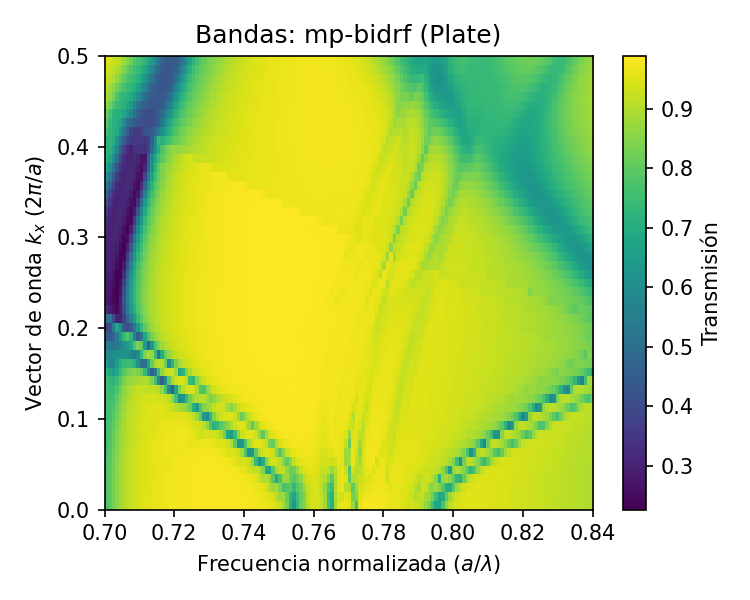
\includegraphics[width=0.48\textwidth]{figures/mp-bidrf_plate.png}
\hfill
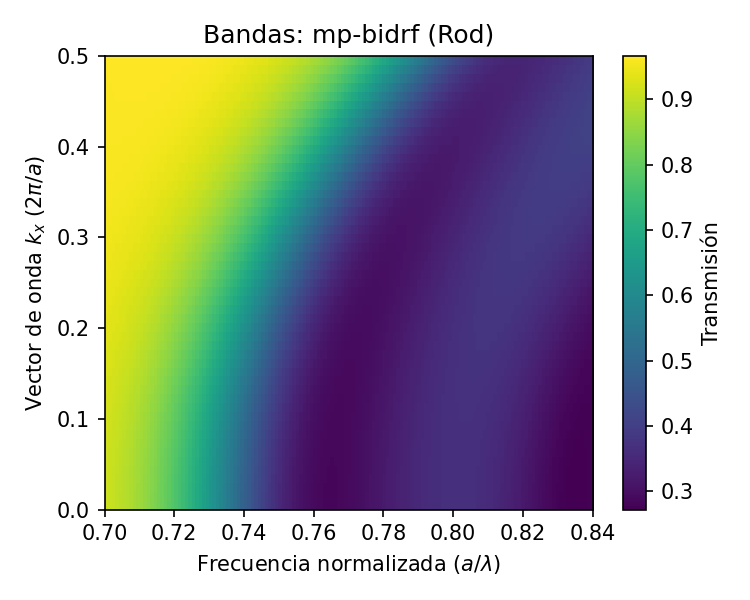
\includegraphics[width=0.48\textwidth]{figures/mp-bidrf_rod.png}
\caption{Estructuras de bandas fotónicas ($k_x$) para mp-bidrf. Izquierda: Lámina. Derecha: Cilindros.}
\end{figure}
\vspace{1em}
\begin{figure}[H]
\centering
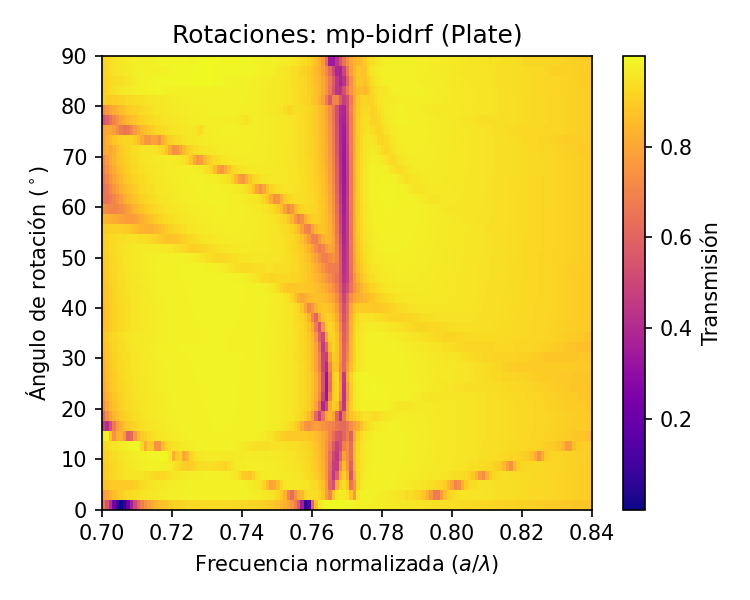
\includegraphics[width=0.48\textwidth]{figures/mp-bidrf_plate_rangle.png}
\hfill
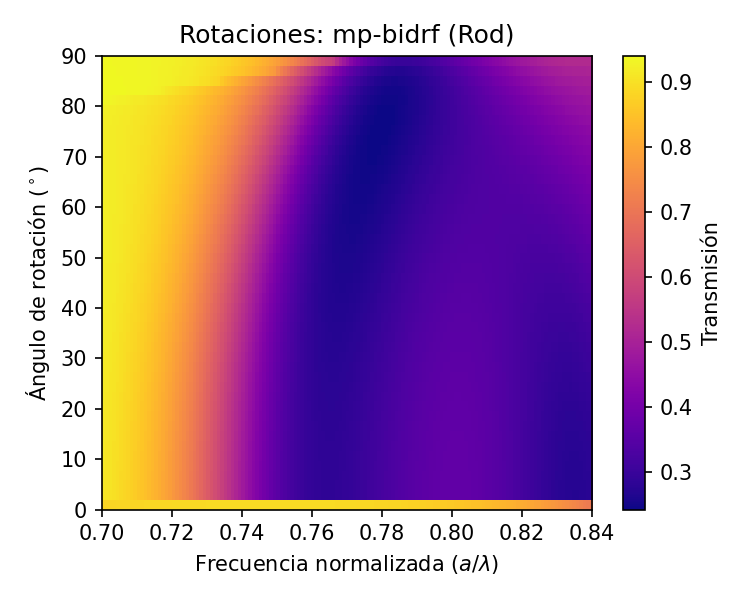
\includegraphics[width=0.48\textwidth]{figures/mp-bidrf_rod_rangle.png}
\caption{Mapas de transmisión por rotación (twist) para mp-bidrf. Izquierda: Lámina. Derecha: Cilindros.}
\end{figure}
\vspace{1em}
\hrule
\vspace{1em}
\subsection*{Material ID: mp-bkjyt}
\textbf{Constante Dieléctrica ($\epsilon_{total}$):} 3.54 \\[0.5em]
\begin{table}[h!]
\centering
\begin{tabular}{lcc}
\toprule
\textbf{Métrica} & \textbf{Lámina (Plate)} & \textbf{Cilindros (Rod)} \\
\midrule
Bandgaps ($k_x$) & Ninguno & Ninguno \\
Resonancias ($k_x$) & 36 & 36 \\
\midrule
Bandgaps (Rotación) & Ninguno & Ninguno \\
Resonancias (Rotación) & 33 & 33 \\
\bottomrule
\end{tabular}
\end{table}
\begin{figure}[H]
\centering
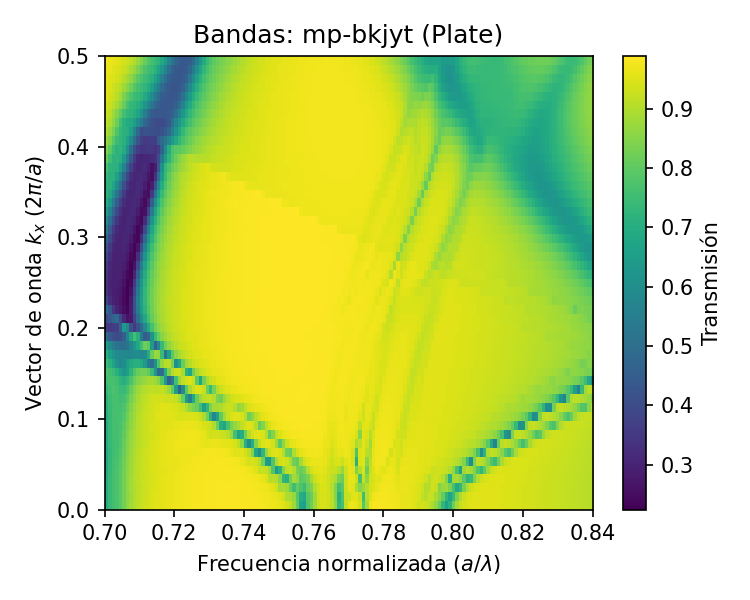
\includegraphics[width=0.48\textwidth]{figures/mp-bkjyt_plate.png}
\hfill
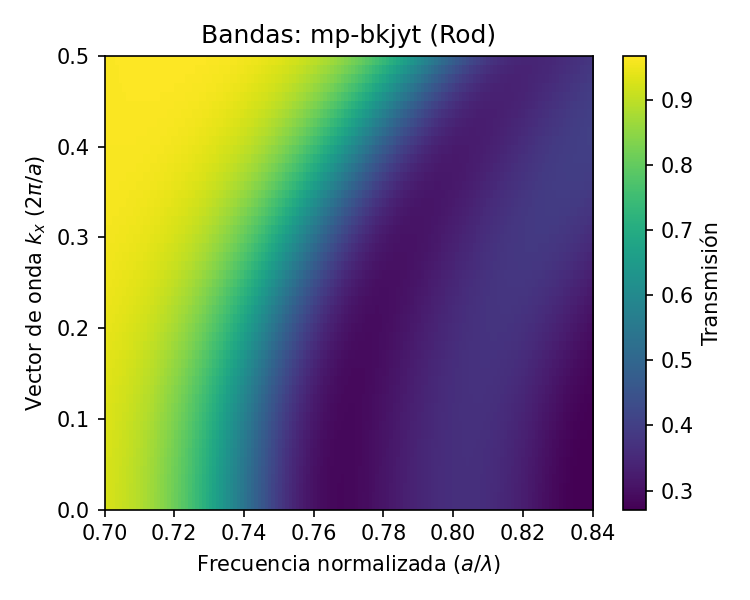
\includegraphics[width=0.48\textwidth]{figures/mp-bkjyt_rod.png}
\caption{Estructuras de bandas fotónicas ($k_x$) para mp-bkjyt. Izquierda: Lámina. Derecha: Cilindros.}
\end{figure}
\vspace{1em}
\begin{figure}[H]
\centering
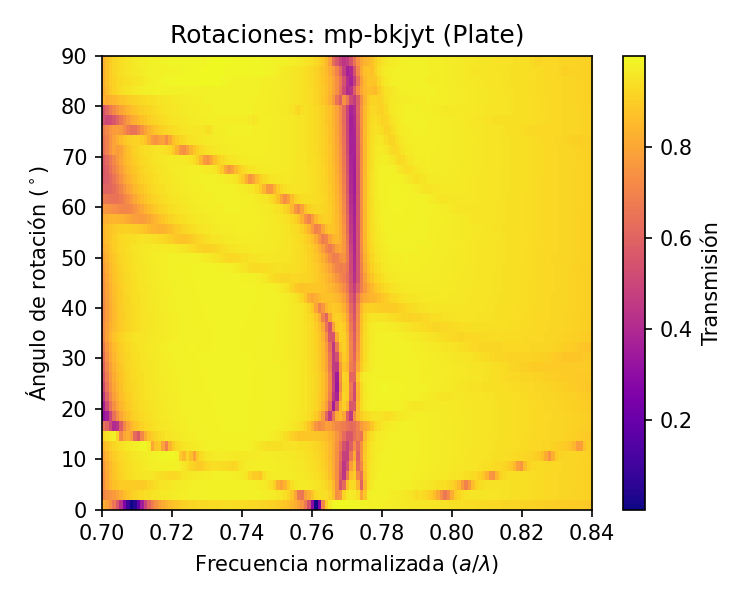
\includegraphics[width=0.48\textwidth]{figures/mp-bkjyt_plate_rangle.png}
\hfill
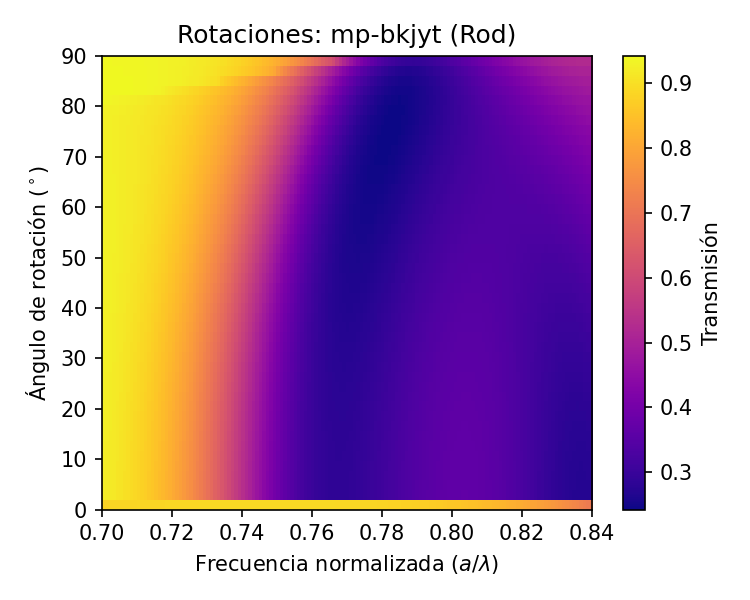
\includegraphics[width=0.48\textwidth]{figures/mp-bkjyt_rod_rangle.png}
\caption{Mapas de transmisión por rotación (twist) para mp-bkjyt. Izquierda: Lámina. Derecha: Cilindros.}
\end{figure}
\vspace{1em}
\hrule
\vspace{1em}
\subsection*{Material ID: mp-bkkhe}
\textbf{Constante Dieléctrica ($\epsilon_{total}$):} 2.93 \\[0.5em]
\begin{table}[h!]
\centering
\begin{tabular}{lcc}
\toprule
\textbf{Métrica} & \textbf{Lámina (Plate)} & \textbf{Cilindros (Rod)} \\
\midrule
Bandgaps ($k_x$) & Ninguno & Ninguno \\
Resonancias ($k_x$) & 36 & 36 \\
\midrule
Bandgaps (Rotación) & Ninguno & Ninguno \\
Resonancias (Rotación) & 33 & 33 \\
\bottomrule
\end{tabular}
\end{table}
\begin{figure}[H]
\centering
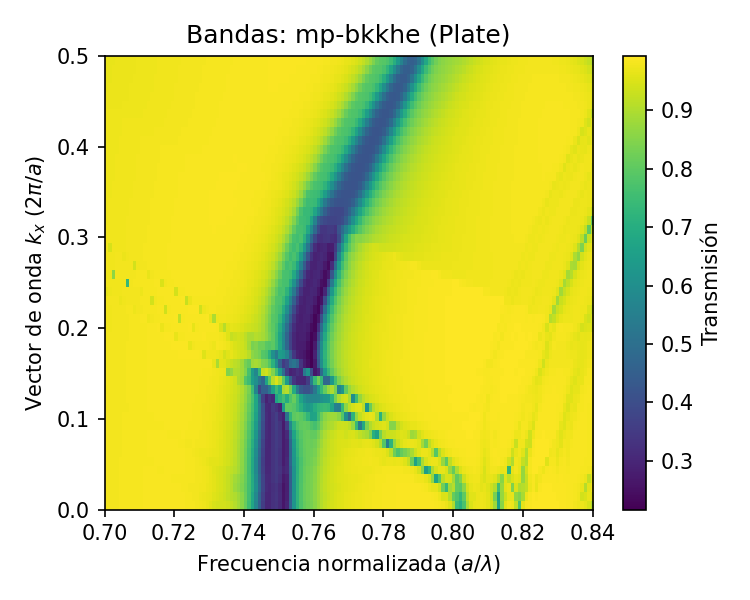
\includegraphics[width=0.48\textwidth]{figures/mp-bkkhe_plate.png}
\hfill
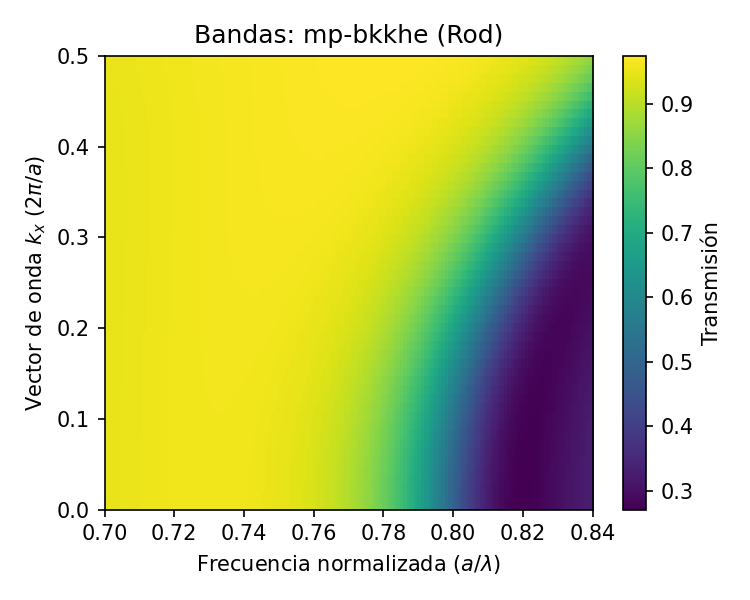
\includegraphics[width=0.48\textwidth]{figures/mp-bkkhe_rod.png}
\caption{Estructuras de bandas fotónicas ($k_x$) para mp-bkkhe. Izquierda: Lámina. Derecha: Cilindros.}
\end{figure}
\vspace{1em}
\begin{figure}[H]
\centering
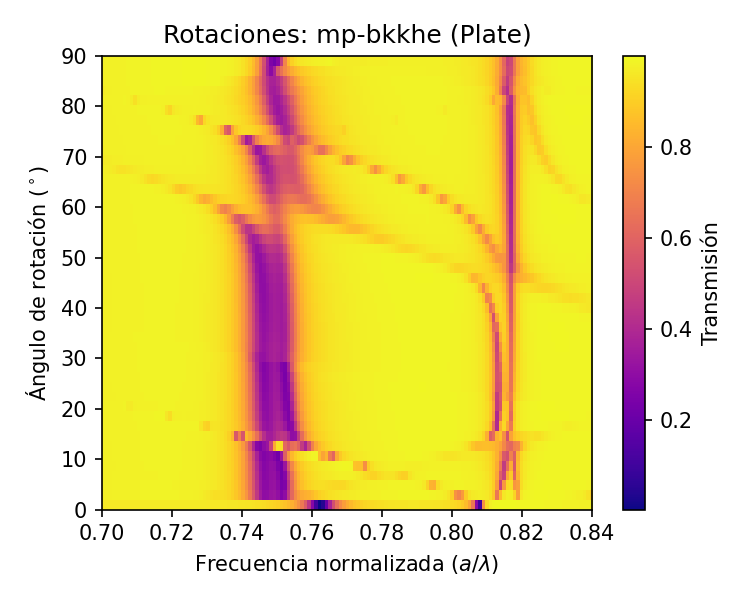
\includegraphics[width=0.48\textwidth]{figures/mp-bkkhe_plate_rangle.png}
\hfill
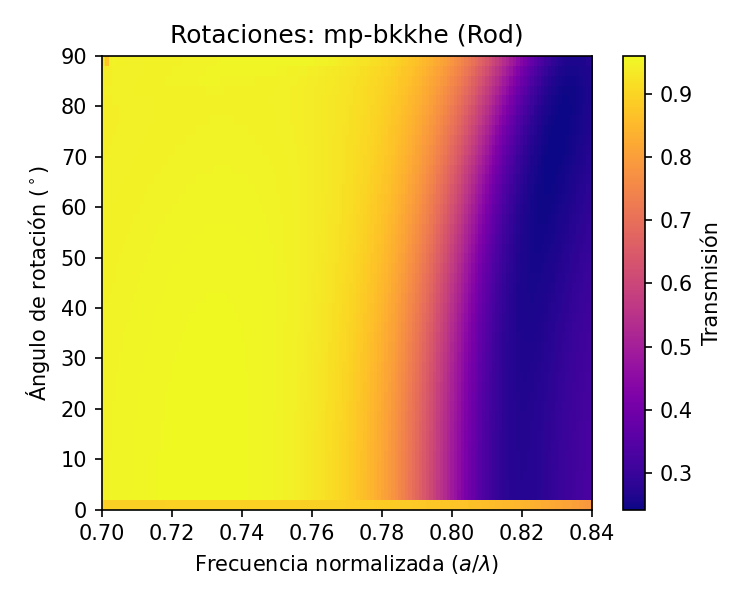
\includegraphics[width=0.48\textwidth]{figures/mp-bkkhe_rod_rangle.png}
\caption{Mapas de transmisión por rotación (twist) para mp-bkkhe. Izquierda: Lámina. Derecha: Cilindros.}
\end{figure}
\vspace{1em}
\hrule
\vspace{1em}
\subsection*{Material ID: mp-bmche}
\textbf{Constante Dieléctrica ($\epsilon_{total}$):} 4.22 \\[0.5em]
\begin{table}[h!]
\centering
\begin{tabular}{lcc}
\toprule
\textbf{Métrica} & \textbf{Lámina (Plate)} & \textbf{Cilindros (Rod)} \\
\midrule
Bandgaps ($k_x$) & Ninguno & Ninguno \\
Resonancias ($k_x$) & 36 & 36 \\
\midrule
Bandgaps (Rotación) & Ninguno & Ninguno \\
Resonancias (Rotación) & 33 & 33 \\
\bottomrule
\end{tabular}
\end{table}
\begin{figure}[H]
\centering
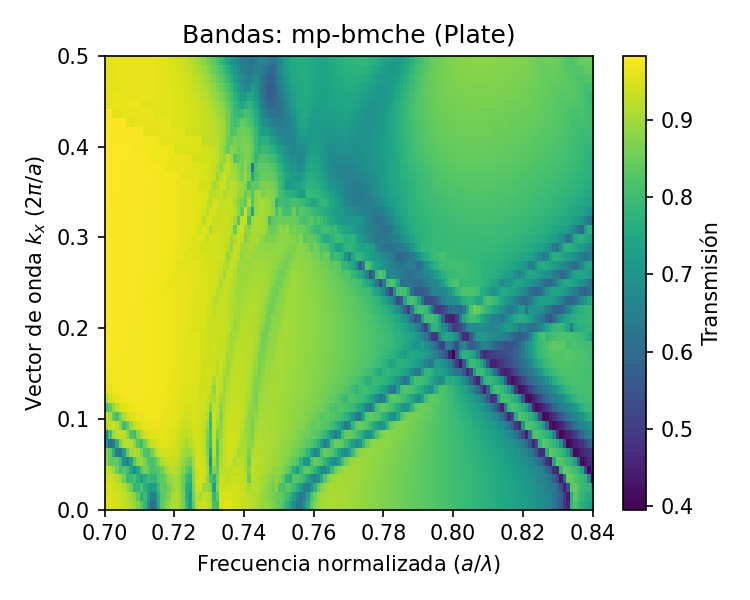
\includegraphics[width=0.48\textwidth]{figures/mp-bmche_plate.png}
\hfill
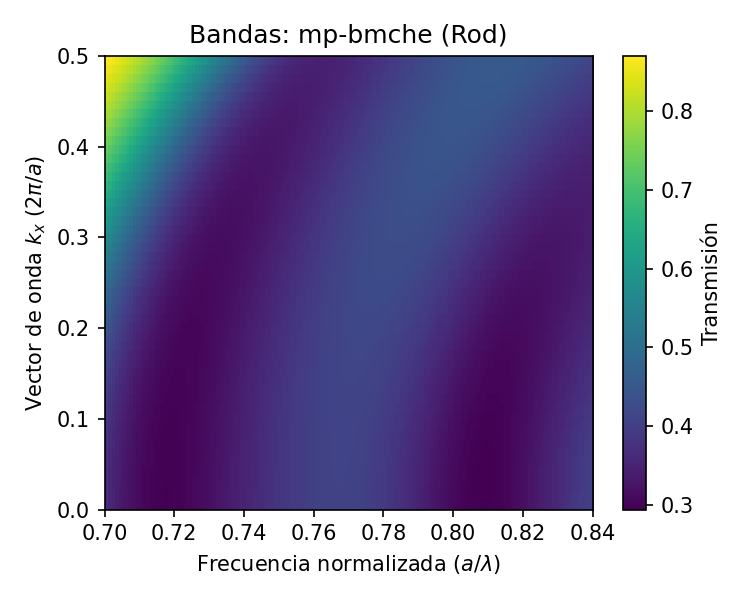
\includegraphics[width=0.48\textwidth]{figures/mp-bmche_rod.png}
\caption{Estructuras de bandas fotónicas ($k_x$) para mp-bmche. Izquierda: Lámina. Derecha: Cilindros.}
\end{figure}
\vspace{1em}
\begin{figure}[H]
\centering
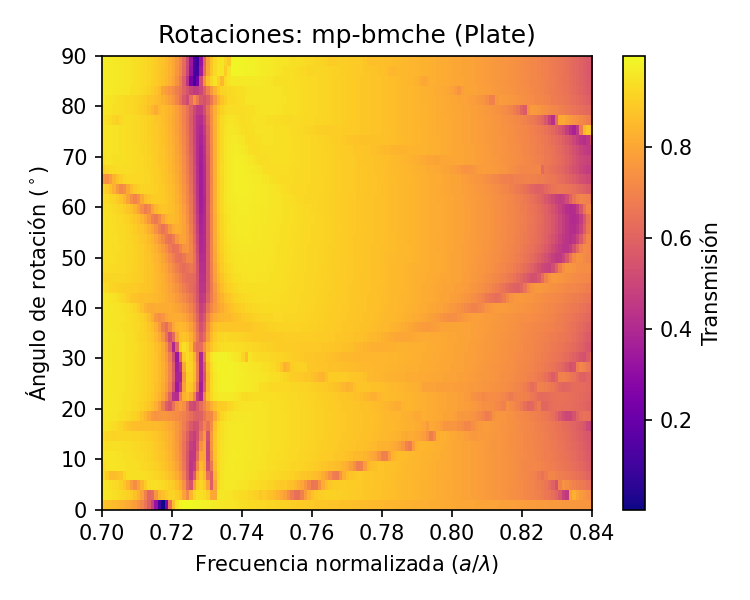
\includegraphics[width=0.48\textwidth]{figures/mp-bmche_plate_rangle.png}
\hfill
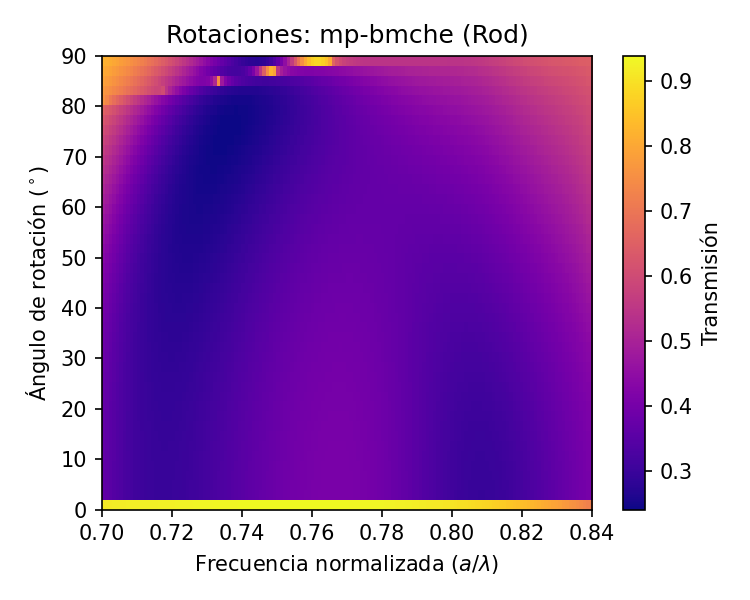
\includegraphics[width=0.48\textwidth]{figures/mp-bmche_rod_rangle.png}
\caption{Mapas de transmisión por rotación (twist) para mp-bmche. Izquierda: Lámina. Derecha: Cilindros.}
\end{figure}
\vspace{1em}
\hrule
\vspace{1em}
\subsection*{Material ID: mp-cdjbs}
\textbf{Constante Dieléctrica ($\epsilon_{total}$):} 4.19 \\[0.5em]
\begin{table}[h!]
\centering
\begin{tabular}{lcc}
\toprule
\textbf{Métrica} & \textbf{Lámina (Plate)} & \textbf{Cilindros (Rod)} \\
\midrule
Bandgaps ($k_x$) & Ninguno & Ninguno \\
Resonancias ($k_x$) & 36 & 36 \\
\midrule
Bandgaps (Rotación) & Ninguno & Ninguno \\
Resonancias (Rotación) & 33 & 33 \\
\bottomrule
\end{tabular}
\end{table}
\begin{figure}[H]
\centering
\includegraphics[width=0.48\textwidth]{figures/mp-cdjbs_plate.png}
\hfill
\includegraphics[width=0.48\textwidth]{figures/mp-cdjbs_rod.png}
\caption{Estructuras de bandas fotónicas ($k_x$) para mp-cdjbs. Izquierda: Lámina. Derecha: Cilindros.}
\end{figure}
\vspace{1em}
\begin{figure}[H]
\centering
\includegraphics[width=0.48\textwidth]{figures/mp-cdjbs_plate_rangle.png}
\hfill
\includegraphics[width=0.48\textwidth]{figures/mp-cdjbs_rod_rangle.png}
\caption{Mapas de transmisión por rotación (twist) para mp-cdjbs. Izquierda: Lámina. Derecha: Cilindros.}
\end{figure}
\vspace{1em}
\hrule
\vspace{1em}
\subsection*{Material ID: mp-kgg}
\textbf{Constante Dieléctrica ($\epsilon_{total}$):} 4.52 \\[0.5em]
\begin{table}[h!]
\centering
\begin{tabular}{lcc}
\toprule
\textbf{Métrica} & \textbf{Lámina (Plate)} & \textbf{Cilindros (Rod)} \\
\midrule
Bandgaps ($k_x$) & Ninguno & Ninguno \\
Resonancias ($k_x$) & 36 & 36 \\
\midrule
Bandgaps (Rotación) & Ninguno & Ninguno \\
Resonancias (Rotación) & 33 & 33 \\
\bottomrule
\end{tabular}
\end{table}
\begin{figure}[H]
\centering
\includegraphics[width=0.48\textwidth]{figures/mp-kgg_plate.png}
\hfill
\includegraphics[width=0.48\textwidth]{figures/mp-kgg_rod.png}
\caption{Estructuras de bandas fotónicas ($k_x$) para mp-kgg. Izquierda: Lámina. Derecha: Cilindros.}
\end{figure}
\vspace{1em}
\begin{figure}[H]
\centering
\includegraphics[width=0.48\textwidth]{figures/mp-kgg_plate_rangle.png}
\hfill
\includegraphics[width=0.48\textwidth]{figures/mp-kgg_rod_rangle.png}
\caption{Mapas de transmisión por rotación (twist) para mp-kgg. Izquierda: Lámina. Derecha: Cilindros.}
\end{figure}
\vspace{1em}
\hrule
\vspace{1em}
\subsection*{Material ID: mp-kgo}
\textbf{Constante Dieléctrica ($\epsilon_{total}$):} 4.73 \\[0.5em]
\begin{table}[h!]
\centering
\begin{tabular}{lcc}
\toprule
\textbf{Métrica} & \textbf{Lámina (Plate)} & \textbf{Cilindros (Rod)} \\
\midrule
Bandgaps ($k_x$) & Ninguno & Ninguno \\
Resonancias ($k_x$) & 36 & 36 \\
\midrule
Bandgaps (Rotación) & Ninguno & Ninguno \\
Resonancias (Rotación) & 33 & 33 \\
\bottomrule
\end{tabular}
\end{table}
\begin{figure}[H]
\centering
\includegraphics[width=0.48\textwidth]{figures/mp-kgo_plate.png}
\hfill
\includegraphics[width=0.48\textwidth]{figures/mp-kgo_rod.png}
\caption{Estructuras de bandas fotónicas ($k_x$) para mp-kgo. Izquierda: Lámina. Derecha: Cilindros.}
\end{figure}
\vspace{1em}
\begin{figure}[H]
\centering
\includegraphics[width=0.48\textwidth]{figures/mp-kgo_plate_rangle.png}
\hfill
\includegraphics[width=0.48\textwidth]{figures/mp-kgo_rod_rangle.png}
\caption{Mapas de transmisión por rotación (twist) para mp-kgo. Izquierda: Lámina. Derecha: Cilindros.}
\end{figure}
\vspace{1em}
\hrule
\vspace{1em}
\subsection*{Material ID: mp-khd}
\textbf{Constante Dieléctrica ($\epsilon_{total}$):} 4.04 \\[0.5em]
\begin{table}[h!]
\centering
\begin{tabular}{lcc}
\toprule
\textbf{Métrica} & \textbf{Lámina (Plate)} & \textbf{Cilindros (Rod)} \\
\midrule
Bandgaps ($k_x$) & Ninguno & Ninguno \\
Resonancias ($k_x$) & 36 & 36 \\
\midrule
Bandgaps (Rotación) & Ninguno & Ninguno \\
Resonancias (Rotación) & 33 & 33 \\
\bottomrule
\end{tabular}
\end{table}
\begin{figure}[H]
\centering
\includegraphics[width=0.48\textwidth]{figures/mp-khd_plate.png}
\hfill
\includegraphics[width=0.48\textwidth]{figures/mp-khd_rod.png}
\caption{Estructuras de bandas fotónicas ($k_x$) para mp-khd. Izquierda: Lámina. Derecha: Cilindros.}
\end{figure}
\vspace{1em}
\begin{figure}[H]
\centering
\includegraphics[width=0.48\textwidth]{figures/mp-khd_plate_rangle.png}
\hfill
\includegraphics[width=0.48\textwidth]{figures/mp-khd_rod_rangle.png}
\caption{Mapas de transmisión por rotación (twist) para mp-khd. Izquierda: Lámina. Derecha: Cilindros.}
\end{figure}
\vspace{1em}
\hrule
\vspace{1em}
\subsection*{Material ID: mp-kjg}
\textbf{Constante Dieléctrica ($\epsilon_{total}$):} 4.59 \\[0.5em]
\begin{table}[h!]
\centering
\begin{tabular}{lcc}
\toprule
\textbf{Métrica} & \textbf{Lámina (Plate)} & \textbf{Cilindros (Rod)} \\
\midrule
Bandgaps ($k_x$) & Ninguno & Ninguno \\
Resonancias ($k_x$) & 36 & 36 \\
\midrule
Bandgaps (Rotación) & Ninguno & Ninguno \\
Resonancias (Rotación) & 33 & 33 \\
\bottomrule
\end{tabular}
\end{table}
\begin{figure}[H]
\centering
\includegraphics[width=0.48\textwidth]{figures/mp-kjg_plate.png}
\hfill
\includegraphics[width=0.48\textwidth]{figures/mp-kjg_rod.png}
\caption{Estructuras de bandas fotónicas ($k_x$) para mp-kjg. Izquierda: Lámina. Derecha: Cilindros.}
\end{figure}
\vspace{1em}
\begin{figure}[H]
\centering
\includegraphics[width=0.48\textwidth]{figures/mp-kjg_plate_rangle.png}
\hfill
\includegraphics[width=0.48\textwidth]{figures/mp-kjg_rod_rangle.png}
\caption{Mapas de transmisión por rotación (twist) para mp-kjg. Izquierda: Lámina. Derecha: Cilindros.}
\end{figure}
\vspace{1em}
\hrule
\vspace{1em}
\subsection*{Material ID: mp-kkj}
\textbf{Constante Dieléctrica ($\epsilon_{total}$):} 4.01 \\[0.5em]
\begin{table}[h!]
\centering
\begin{tabular}{lcc}
\toprule
\textbf{Métrica} & \textbf{Lámina (Plate)} & \textbf{Cilindros (Rod)} \\
\midrule
Bandgaps ($k_x$) & Ninguno & Ninguno \\
Resonancias ($k_x$) & 36 & 36 \\
\midrule
Bandgaps (Rotación) & Ninguno & Ninguno \\
Resonancias (Rotación) & 33 & 33 \\
\bottomrule
\end{tabular}
\end{table}
\begin{figure}[H]
\centering
\includegraphics[width=0.48\textwidth]{figures/mp-kkj_plate.png}
\hfill
\includegraphics[width=0.48\textwidth]{figures/mp-kkj_rod.png}
\caption{Estructuras de bandas fotónicas ($k_x$) para mp-kkj. Izquierda: Lámina. Derecha: Cilindros.}
\end{figure}
\vspace{1em}
\begin{figure}[H]
\centering
\includegraphics[width=0.48\textwidth]{figures/mp-kkj_plate_rangle.png}
\hfill
\includegraphics[width=0.48\textwidth]{figures/mp-kkj_rod_rangle.png}
\caption{Mapas de transmisión por rotación (twist) para mp-kkj. Izquierda: Lámina. Derecha: Cilindros.}
\end{figure}
\vspace{1em}
\hrule
\vspace{1em}
\subsection*{Material ID: mp-lie}
\textbf{Constante Dieléctrica ($\epsilon_{total}$):} 12.74 \\[0.5em]
\begin{table}[h!]
\centering
\begin{tabular}{lcc}
\toprule
\textbf{Métrica} & \textbf{Lámina (Plate)} & \textbf{Cilindros (Rod)} \\
\midrule
Bandgaps ($k_x$) & Ninguno & Ninguno \\
Resonancias ($k_x$) & 36 & 36 \\
\midrule
Bandgaps (Rotación) & Ninguno & Ninguno \\
Resonancias (Rotación) & 33 & 33 \\
\bottomrule
\end{tabular}
\end{table}
\begin{figure}[H]
\centering
\includegraphics[width=0.48\textwidth]{figures/mp-lie_plate.png}
\hfill
\includegraphics[width=0.48\textwidth]{figures/mp-lie_rod.png}
\caption{Estructuras de bandas fotónicas ($k_x$) para mp-lie. Izquierda: Lámina. Derecha: Cilindros.}
\end{figure}
\vspace{1em}
\begin{figure}[H]
\centering
\includegraphics[width=0.48\textwidth]{figures/mp-lie_plate_rangle.png}
\hfill
\includegraphics[width=0.48\textwidth]{figures/mp-lie_rod_rangle.png}
\caption{Mapas de transmisión por rotación (twist) para mp-lie. Izquierda: Lámina. Derecha: Cilindros.}
\end{figure}
\vspace{1em}
\hrule
\vspace{1em}
\subsection*{Material ID: mp-lxz}
\textbf{Constante Dieléctrica ($\epsilon_{total}$):} 3.94 \\[0.5em]
\begin{table}[h!]
\centering
\begin{tabular}{lcc}
\toprule
\textbf{Métrica} & \textbf{Lámina (Plate)} & \textbf{Cilindros (Rod)} \\
\midrule
Bandgaps ($k_x$) & Ninguno & Ninguno \\
Resonancias ($k_x$) & 36 & 36 \\
\midrule
Bandgaps (Rotación) & Ninguno & Ninguno \\
Resonancias (Rotación) & 33 & 33 \\
\bottomrule
\end{tabular}
\end{table}
\begin{figure}[H]
\centering
\includegraphics[width=0.48\textwidth]{figures/mp-lxz_plate.png}
\hfill
\includegraphics[width=0.48\textwidth]{figures/mp-lxz_rod.png}
\caption{Estructuras de bandas fotónicas ($k_x$) para mp-lxz. Izquierda: Lámina. Derecha: Cilindros.}
\end{figure}
\vspace{1em}
\begin{figure}[H]
\centering
\includegraphics[width=0.48\textwidth]{figures/mp-lxz_plate_rangle.png}
\hfill
\includegraphics[width=0.48\textwidth]{figures/mp-lxz_rod_rangle.png}
\caption{Mapas de transmisión por rotación (twist) para mp-lxz. Izquierda: Lámina. Derecha: Cilindros.}
\end{figure}
\vspace{1em}
\hrule
\vspace{1em}
\subsection*{Material ID: mp-qbj}
\textbf{Constante Dieléctrica ($\epsilon_{total}$):} 4.52 \\[0.5em]
\begin{table}[h!]
\centering
\begin{tabular}{lcc}
\toprule
\textbf{Métrica} & \textbf{Lámina (Plate)} & \textbf{Cilindros (Rod)} \\
\midrule
Bandgaps ($k_x$) & Ninguno & Ninguno \\
Resonancias ($k_x$) & 36 & 36 \\
\midrule
Bandgaps (Rotación) & Ninguno & Ninguno \\
Resonancias (Rotación) & 33 & 33 \\
\bottomrule
\end{tabular}
\end{table}
\begin{figure}[H]
\centering
\includegraphics[width=0.48\textwidth]{figures/mp-qbj_plate.png}
\hfill
\includegraphics[width=0.48\textwidth]{figures/mp-qbj_rod.png}
\caption{Estructuras de bandas fotónicas ($k_x$) para mp-qbj. Izquierda: Lámina. Derecha: Cilindros.}
\end{figure}
\vspace{1em}
\begin{figure}[H]
\centering
\includegraphics[width=0.48\textwidth]{figures/mp-qbj_plate_rangle.png}
\hfill
\includegraphics[width=0.48\textwidth]{figures/mp-qbj_rod_rangle.png}
\caption{Mapas de transmisión por rotación (twist) para mp-qbj. Izquierda: Lámina. Derecha: Cilindros.}
\end{figure}
\vspace{1em}
\hrule
\vspace{1em}
\subsection*{Material ID: mp-zcm}
\textbf{Constante Dieléctrica ($\epsilon_{total}$):} 3.54 \\[0.5em]
\begin{table}[h!]
\centering
\begin{tabular}{lcc}
\toprule
\textbf{Métrica} & \textbf{Lámina (Plate)} & \textbf{Cilindros (Rod)} \\
\midrule
Bandgaps ($k_x$) & Ninguno & Ninguno \\
Resonancias ($k_x$) & 36 & 36 \\
\midrule
Bandgaps (Rotación) & Ninguno & Ninguno \\
Resonancias (Rotación) & 33 & 33 \\
\bottomrule
\end{tabular}
\end{table}
\begin{figure}[H]
\centering
\includegraphics[width=0.48\textwidth]{figures/mp-zcm_plate.png}
\hfill
\includegraphics[width=0.48\textwidth]{figures/mp-zcm_rod.png}
\caption{Estructuras de bandas fotónicas ($k_x$) para mp-zcm. Izquierda: Lámina. Derecha: Cilindros.}
\end{figure}
\vspace{1em}
\begin{figure}[H]
\centering
\includegraphics[width=0.48\textwidth]{figures/mp-zcm_plate_rangle.png}
\hfill
\includegraphics[width=0.48\textwidth]{figures/mp-zcm_rod_rangle.png}
\caption{Mapas de transmisión por rotación (twist) para mp-zcm. Izquierda: Lámina. Derecha: Cilindros.}
\end{figure}
\vspace{1em}
\hrule
\vspace{1em}
\clearpage